\documentclass[11pt]{article}

    \usepackage[breakable]{tcolorbox}
    \usepackage{parskip} % Stop auto-indenting (to mimic markdown behaviour)
    

    % Basic figure setup, for now with no caption control since it's done
    % automatically by Pandoc (which extracts ![](path) syntax from Markdown).
    \usepackage{graphicx}
    % Keep aspect ratio if custom image width or height is specified
    \setkeys{Gin}{keepaspectratio}
    % Maintain compatibility with old templates. Remove in nbconvert 6.0
    \let\Oldincludegraphics\includegraphics
    % Ensure that by default, figures have no caption (until we provide a
    % proper Figure object with a Caption API and a way to capture that
    % in the conversion process - todo).
    \usepackage{caption}
    \DeclareCaptionFormat{nocaption}{}
    \captionsetup{format=nocaption,aboveskip=0pt,belowskip=0pt}

    \usepackage{float}
    \floatplacement{figure}{H} % forces figures to be placed at the correct location
    \usepackage{xcolor} % Allow colors to be defined
    \usepackage{enumerate} % Needed for markdown enumerations to work
    \usepackage{geometry} % Used to adjust the document margins
    \usepackage{amsmath} % Equations
    \usepackage{amssymb} % Equations
    \usepackage{textcomp} % defines textquotesingle
    % Hack from http://tex.stackexchange.com/a/47451/13684:
    \AtBeginDocument{%
        \def\PYZsq{\textquotesingle}% Upright quotes in Pygmentized code
    }
    \usepackage{upquote} % Upright quotes for verbatim code
    \usepackage{eurosym} % defines \euro

    \usepackage{iftex}
    \ifPDFTeX
        \usepackage[T1]{fontenc}
        \IfFileExists{alphabeta.sty}{
              \usepackage{alphabeta}
          }{
              \usepackage[mathletters]{ucs}
              \usepackage[utf8x]{inputenc}
          }
    \else
        \usepackage{fontspec}
        \usepackage{unicode-math}
    \fi

    \usepackage{fancyvrb} % verbatim replacement that allows latex
    \usepackage{grffile} % extends the file name processing of package graphics
                         % to support a larger range
    \makeatletter % fix for old versions of grffile with XeLaTeX
    \@ifpackagelater{grffile}{2019/11/01}
    {
      % Do nothing on new versions
    }
    {
      \def\Gread@@xetex#1{%
        \IfFileExists{"\Gin@base".bb}%
        {\Gread@eps{\Gin@base.bb}}%
        {\Gread@@xetex@aux#1}%
      }
    }
    \makeatother
    \usepackage[Export]{adjustbox} % Used to constrain images to a maximum size
    \adjustboxset{max size={0.9\linewidth}{0.9\paperheight}}

    % The hyperref package gives us a pdf with properly built
    % internal navigation ('pdf bookmarks' for the table of contents,
    % internal cross-reference links, web links for URLs, etc.)
    \usepackage{hyperref}
    % The default LaTeX title has an obnoxious amount of whitespace. By default,
    % titling removes some of it. It also provides customization options.
    \usepackage{titling}
    \usepackage{longtable} % longtable support required by pandoc >1.10
    \usepackage{booktabs}  % table support for pandoc > 1.12.2
    \usepackage{array}     % table support for pandoc >= 2.11.3
    \usepackage{calc}      % table minipage width calculation for pandoc >= 2.11.1
    \usepackage[inline]{enumitem} % IRkernel/repr support (it uses the enumerate* environment)
    \usepackage[normalem]{ulem} % ulem is needed to support strikethroughs (\sout)
                                % normalem makes italics be italics, not underlines
    \usepackage{soul}      % strikethrough (\st) support for pandoc >= 3.0.0
    \usepackage{mathrsfs}
    

    
    % Colors for the hyperref package
    \definecolor{urlcolor}{rgb}{0,.145,.698}
    \definecolor{linkcolor}{rgb}{.71,0.21,0.01}
    \definecolor{citecolor}{rgb}{.12,.54,.11}

    % ANSI colors
    \definecolor{ansi-black}{HTML}{3E424D}
    \definecolor{ansi-black-intense}{HTML}{282C36}
    \definecolor{ansi-red}{HTML}{E75C58}
    \definecolor{ansi-red-intense}{HTML}{B22B31}
    \definecolor{ansi-green}{HTML}{00A250}
    \definecolor{ansi-green-intense}{HTML}{007427}
    \definecolor{ansi-yellow}{HTML}{DDB62B}
    \definecolor{ansi-yellow-intense}{HTML}{B27D12}
    \definecolor{ansi-blue}{HTML}{208FFB}
    \definecolor{ansi-blue-intense}{HTML}{0065CA}
    \definecolor{ansi-magenta}{HTML}{D160C4}
    \definecolor{ansi-magenta-intense}{HTML}{A03196}
    \definecolor{ansi-cyan}{HTML}{60C6C8}
    \definecolor{ansi-cyan-intense}{HTML}{258F8F}
    \definecolor{ansi-white}{HTML}{C5C1B4}
    \definecolor{ansi-white-intense}{HTML}{A1A6B2}
    \definecolor{ansi-default-inverse-fg}{HTML}{FFFFFF}
    \definecolor{ansi-default-inverse-bg}{HTML}{000000}

    % common color for the border for error outputs.
    \definecolor{outerrorbackground}{HTML}{FFDFDF}

    % commands and environments needed by pandoc snippets
    % extracted from the output of `pandoc -s`
    \providecommand{\tightlist}{%
      \setlength{\itemsep}{0pt}\setlength{\parskip}{0pt}}
    \DefineVerbatimEnvironment{Highlighting}{Verbatim}{commandchars=\\\{\}}
    % Add ',fontsize=\small' for more characters per line
    \newenvironment{Shaded}{}{}
    \newcommand{\KeywordTok}[1]{\textcolor[rgb]{0.00,0.44,0.13}{\textbf{{#1}}}}
    \newcommand{\DataTypeTok}[1]{\textcolor[rgb]{0.56,0.13,0.00}{{#1}}}
    \newcommand{\DecValTok}[1]{\textcolor[rgb]{0.25,0.63,0.44}{{#1}}}
    \newcommand{\BaseNTok}[1]{\textcolor[rgb]{0.25,0.63,0.44}{{#1}}}
    \newcommand{\FloatTok}[1]{\textcolor[rgb]{0.25,0.63,0.44}{{#1}}}
    \newcommand{\CharTok}[1]{\textcolor[rgb]{0.25,0.44,0.63}{{#1}}}
    \newcommand{\StringTok}[1]{\textcolor[rgb]{0.25,0.44,0.63}{{#1}}}
    \newcommand{\CommentTok}[1]{\textcolor[rgb]{0.38,0.63,0.69}{\textit{{#1}}}}
    \newcommand{\OtherTok}[1]{\textcolor[rgb]{0.00,0.44,0.13}{{#1}}}
    \newcommand{\AlertTok}[1]{\textcolor[rgb]{1.00,0.00,0.00}{\textbf{{#1}}}}
    \newcommand{\FunctionTok}[1]{\textcolor[rgb]{0.02,0.16,0.49}{{#1}}}
    \newcommand{\RegionMarkerTok}[1]{{#1}}
    \newcommand{\ErrorTok}[1]{\textcolor[rgb]{1.00,0.00,0.00}{\textbf{{#1}}}}
    \newcommand{\NormalTok}[1]{{#1}}

    % Additional commands for more recent versions of Pandoc
    \newcommand{\ConstantTok}[1]{\textcolor[rgb]{0.53,0.00,0.00}{{#1}}}
    \newcommand{\SpecialCharTok}[1]{\textcolor[rgb]{0.25,0.44,0.63}{{#1}}}
    \newcommand{\VerbatimStringTok}[1]{\textcolor[rgb]{0.25,0.44,0.63}{{#1}}}
    \newcommand{\SpecialStringTok}[1]{\textcolor[rgb]{0.73,0.40,0.53}{{#1}}}
    \newcommand{\ImportTok}[1]{{#1}}
    \newcommand{\DocumentationTok}[1]{\textcolor[rgb]{0.73,0.13,0.13}{\textit{{#1}}}}
    \newcommand{\AnnotationTok}[1]{\textcolor[rgb]{0.38,0.63,0.69}{\textbf{\textit{{#1}}}}}
    \newcommand{\CommentVarTok}[1]{\textcolor[rgb]{0.38,0.63,0.69}{\textbf{\textit{{#1}}}}}
    \newcommand{\VariableTok}[1]{\textcolor[rgb]{0.10,0.09,0.49}{{#1}}}
    \newcommand{\ControlFlowTok}[1]{\textcolor[rgb]{0.00,0.44,0.13}{\textbf{{#1}}}}
    \newcommand{\OperatorTok}[1]{\textcolor[rgb]{0.40,0.40,0.40}{{#1}}}
    \newcommand{\BuiltInTok}[1]{{#1}}
    \newcommand{\ExtensionTok}[1]{{#1}}
    \newcommand{\PreprocessorTok}[1]{\textcolor[rgb]{0.74,0.48,0.00}{{#1}}}
    \newcommand{\AttributeTok}[1]{\textcolor[rgb]{0.49,0.56,0.16}{{#1}}}
    \newcommand{\InformationTok}[1]{\textcolor[rgb]{0.38,0.63,0.69}{\textbf{\textit{{#1}}}}}
    \newcommand{\WarningTok}[1]{\textcolor[rgb]{0.38,0.63,0.69}{\textbf{\textit{{#1}}}}}


    % Define a nice break command that doesn't care if a line doesn't already
    % exist.
    \def\br{\hspace*{\fill} \\* }
    % Math Jax compatibility definitions
    \def\gt{>}
    \def\lt{<}
    \let\Oldtex\TeX
    \let\Oldlatex\LaTeX
    \renewcommand{\TeX}{\textrm{\Oldtex}}
    \renewcommand{\LaTeX}{\textrm{\Oldlatex}}
    % Document parameters
    % Document title
    \title{COSE474-2024F: Deep Learning HW1}
    \author{Jaehoon Han, 2022320101}
    
    
    
    
    
    
    
% Pygments definitions
\makeatletter
\def\PY@reset{\let\PY@it=\relax \let\PY@bf=\relax%
    \let\PY@ul=\relax \let\PY@tc=\relax%
    \let\PY@bc=\relax \let\PY@ff=\relax}
\def\PY@tok#1{\csname PY@tok@#1\endcsname}
\def\PY@toks#1+{\ifx\relax#1\empty\else%
    \PY@tok{#1}\expandafter\PY@toks\fi}
\def\PY@do#1{\PY@bc{\PY@tc{\PY@ul{%
    \PY@it{\PY@bf{\PY@ff{#1}}}}}}}
\def\PY#1#2{\PY@reset\PY@toks#1+\relax+\PY@do{#2}}

\@namedef{PY@tok@w}{\def\PY@tc##1{\textcolor[rgb]{0.73,0.73,0.73}{##1}}}
\@namedef{PY@tok@c}{\let\PY@it=\textit\def\PY@tc##1{\textcolor[rgb]{0.24,0.48,0.48}{##1}}}
\@namedef{PY@tok@cp}{\def\PY@tc##1{\textcolor[rgb]{0.61,0.40,0.00}{##1}}}
\@namedef{PY@tok@k}{\let\PY@bf=\textbf\def\PY@tc##1{\textcolor[rgb]{0.00,0.50,0.00}{##1}}}
\@namedef{PY@tok@kp}{\def\PY@tc##1{\textcolor[rgb]{0.00,0.50,0.00}{##1}}}
\@namedef{PY@tok@kt}{\def\PY@tc##1{\textcolor[rgb]{0.69,0.00,0.25}{##1}}}
\@namedef{PY@tok@o}{\def\PY@tc##1{\textcolor[rgb]{0.40,0.40,0.40}{##1}}}
\@namedef{PY@tok@ow}{\let\PY@bf=\textbf\def\PY@tc##1{\textcolor[rgb]{0.67,0.13,1.00}{##1}}}
\@namedef{PY@tok@nb}{\def\PY@tc##1{\textcolor[rgb]{0.00,0.50,0.00}{##1}}}
\@namedef{PY@tok@nf}{\def\PY@tc##1{\textcolor[rgb]{0.00,0.00,1.00}{##1}}}
\@namedef{PY@tok@nc}{\let\PY@bf=\textbf\def\PY@tc##1{\textcolor[rgb]{0.00,0.00,1.00}{##1}}}
\@namedef{PY@tok@nn}{\let\PY@bf=\textbf\def\PY@tc##1{\textcolor[rgb]{0.00,0.00,1.00}{##1}}}
\@namedef{PY@tok@ne}{\let\PY@bf=\textbf\def\PY@tc##1{\textcolor[rgb]{0.80,0.25,0.22}{##1}}}
\@namedef{PY@tok@nv}{\def\PY@tc##1{\textcolor[rgb]{0.10,0.09,0.49}{##1}}}
\@namedef{PY@tok@no}{\def\PY@tc##1{\textcolor[rgb]{0.53,0.00,0.00}{##1}}}
\@namedef{PY@tok@nl}{\def\PY@tc##1{\textcolor[rgb]{0.46,0.46,0.00}{##1}}}
\@namedef{PY@tok@ni}{\let\PY@bf=\textbf\def\PY@tc##1{\textcolor[rgb]{0.44,0.44,0.44}{##1}}}
\@namedef{PY@tok@na}{\def\PY@tc##1{\textcolor[rgb]{0.41,0.47,0.13}{##1}}}
\@namedef{PY@tok@nt}{\let\PY@bf=\textbf\def\PY@tc##1{\textcolor[rgb]{0.00,0.50,0.00}{##1}}}
\@namedef{PY@tok@nd}{\def\PY@tc##1{\textcolor[rgb]{0.67,0.13,1.00}{##1}}}
\@namedef{PY@tok@s}{\def\PY@tc##1{\textcolor[rgb]{0.73,0.13,0.13}{##1}}}
\@namedef{PY@tok@sd}{\let\PY@it=\textit\def\PY@tc##1{\textcolor[rgb]{0.73,0.13,0.13}{##1}}}
\@namedef{PY@tok@si}{\let\PY@bf=\textbf\def\PY@tc##1{\textcolor[rgb]{0.64,0.35,0.47}{##1}}}
\@namedef{PY@tok@se}{\let\PY@bf=\textbf\def\PY@tc##1{\textcolor[rgb]{0.67,0.36,0.12}{##1}}}
\@namedef{PY@tok@sr}{\def\PY@tc##1{\textcolor[rgb]{0.64,0.35,0.47}{##1}}}
\@namedef{PY@tok@ss}{\def\PY@tc##1{\textcolor[rgb]{0.10,0.09,0.49}{##1}}}
\@namedef{PY@tok@sx}{\def\PY@tc##1{\textcolor[rgb]{0.00,0.50,0.00}{##1}}}
\@namedef{PY@tok@m}{\def\PY@tc##1{\textcolor[rgb]{0.40,0.40,0.40}{##1}}}
\@namedef{PY@tok@gh}{\let\PY@bf=\textbf\def\PY@tc##1{\textcolor[rgb]{0.00,0.00,0.50}{##1}}}
\@namedef{PY@tok@gu}{\let\PY@bf=\textbf\def\PY@tc##1{\textcolor[rgb]{0.50,0.00,0.50}{##1}}}
\@namedef{PY@tok@gd}{\def\PY@tc##1{\textcolor[rgb]{0.63,0.00,0.00}{##1}}}
\@namedef{PY@tok@gi}{\def\PY@tc##1{\textcolor[rgb]{0.00,0.52,0.00}{##1}}}
\@namedef{PY@tok@gr}{\def\PY@tc##1{\textcolor[rgb]{0.89,0.00,0.00}{##1}}}
\@namedef{PY@tok@ge}{\let\PY@it=\textit}
\@namedef{PY@tok@gs}{\let\PY@bf=\textbf}
\@namedef{PY@tok@ges}{\let\PY@bf=\textbf\let\PY@it=\textit}
\@namedef{PY@tok@gp}{\let\PY@bf=\textbf\def\PY@tc##1{\textcolor[rgb]{0.00,0.00,0.50}{##1}}}
\@namedef{PY@tok@go}{\def\PY@tc##1{\textcolor[rgb]{0.44,0.44,0.44}{##1}}}
\@namedef{PY@tok@gt}{\def\PY@tc##1{\textcolor[rgb]{0.00,0.27,0.87}{##1}}}
\@namedef{PY@tok@err}{\def\PY@bc##1{{\setlength{\fboxsep}{\string -\fboxrule}\fcolorbox[rgb]{1.00,0.00,0.00}{1,1,1}{\strut ##1}}}}
\@namedef{PY@tok@kc}{\let\PY@bf=\textbf\def\PY@tc##1{\textcolor[rgb]{0.00,0.50,0.00}{##1}}}
\@namedef{PY@tok@kd}{\let\PY@bf=\textbf\def\PY@tc##1{\textcolor[rgb]{0.00,0.50,0.00}{##1}}}
\@namedef{PY@tok@kn}{\let\PY@bf=\textbf\def\PY@tc##1{\textcolor[rgb]{0.00,0.50,0.00}{##1}}}
\@namedef{PY@tok@kr}{\let\PY@bf=\textbf\def\PY@tc##1{\textcolor[rgb]{0.00,0.50,0.00}{##1}}}
\@namedef{PY@tok@bp}{\def\PY@tc##1{\textcolor[rgb]{0.00,0.50,0.00}{##1}}}
\@namedef{PY@tok@fm}{\def\PY@tc##1{\textcolor[rgb]{0.00,0.00,1.00}{##1}}}
\@namedef{PY@tok@vc}{\def\PY@tc##1{\textcolor[rgb]{0.10,0.09,0.49}{##1}}}
\@namedef{PY@tok@vg}{\def\PY@tc##1{\textcolor[rgb]{0.10,0.09,0.49}{##1}}}
\@namedef{PY@tok@vi}{\def\PY@tc##1{\textcolor[rgb]{0.10,0.09,0.49}{##1}}}
\@namedef{PY@tok@vm}{\def\PY@tc##1{\textcolor[rgb]{0.10,0.09,0.49}{##1}}}
\@namedef{PY@tok@sa}{\def\PY@tc##1{\textcolor[rgb]{0.73,0.13,0.13}{##1}}}
\@namedef{PY@tok@sb}{\def\PY@tc##1{\textcolor[rgb]{0.73,0.13,0.13}{##1}}}
\@namedef{PY@tok@sc}{\def\PY@tc##1{\textcolor[rgb]{0.73,0.13,0.13}{##1}}}
\@namedef{PY@tok@dl}{\def\PY@tc##1{\textcolor[rgb]{0.73,0.13,0.13}{##1}}}
\@namedef{PY@tok@s2}{\def\PY@tc##1{\textcolor[rgb]{0.73,0.13,0.13}{##1}}}
\@namedef{PY@tok@sh}{\def\PY@tc##1{\textcolor[rgb]{0.73,0.13,0.13}{##1}}}
\@namedef{PY@tok@s1}{\def\PY@tc##1{\textcolor[rgb]{0.73,0.13,0.13}{##1}}}
\@namedef{PY@tok@mb}{\def\PY@tc##1{\textcolor[rgb]{0.40,0.40,0.40}{##1}}}
\@namedef{PY@tok@mf}{\def\PY@tc##1{\textcolor[rgb]{0.40,0.40,0.40}{##1}}}
\@namedef{PY@tok@mh}{\def\PY@tc##1{\textcolor[rgb]{0.40,0.40,0.40}{##1}}}
\@namedef{PY@tok@mi}{\def\PY@tc##1{\textcolor[rgb]{0.40,0.40,0.40}{##1}}}
\@namedef{PY@tok@il}{\def\PY@tc##1{\textcolor[rgb]{0.40,0.40,0.40}{##1}}}
\@namedef{PY@tok@mo}{\def\PY@tc##1{\textcolor[rgb]{0.40,0.40,0.40}{##1}}}
\@namedef{PY@tok@ch}{\let\PY@it=\textit\def\PY@tc##1{\textcolor[rgb]{0.24,0.48,0.48}{##1}}}
\@namedef{PY@tok@cm}{\let\PY@it=\textit\def\PY@tc##1{\textcolor[rgb]{0.24,0.48,0.48}{##1}}}
\@namedef{PY@tok@cpf}{\let\PY@it=\textit\def\PY@tc##1{\textcolor[rgb]{0.24,0.48,0.48}{##1}}}
\@namedef{PY@tok@c1}{\let\PY@it=\textit\def\PY@tc##1{\textcolor[rgb]{0.24,0.48,0.48}{##1}}}
\@namedef{PY@tok@cs}{\let\PY@it=\textit\def\PY@tc##1{\textcolor[rgb]{0.24,0.48,0.48}{##1}}}

\def\PYZbs{\char`\\}
\def\PYZus{\char`\_}
\def\PYZob{\char`\{}
\def\PYZcb{\char`\}}
\def\PYZca{\char`\^}
\def\PYZam{\char`\&}
\def\PYZlt{\char`\<}
\def\PYZgt{\char`\>}
\def\PYZsh{\char`\#}
\def\PYZpc{\char`\%}
\def\PYZdl{\char`\$}
\def\PYZhy{\char`\-}
\def\PYZsq{\char`\'}
\def\PYZdq{\char`\"}
\def\PYZti{\char`\~}
% for compatibility with earlier versions
\def\PYZat{@}
\def\PYZlb{[}
\def\PYZrb{]}
\makeatother


    % For linebreaks inside Verbatim environment from package fancyvrb.
    \makeatletter
        \newbox\Wrappedcontinuationbox
        \newbox\Wrappedvisiblespacebox
        \newcommand*\Wrappedvisiblespace {\textcolor{red}{\textvisiblespace}}
        \newcommand*\Wrappedcontinuationsymbol {\textcolor{red}{\llap{\tiny$\m@th\hookrightarrow$}}}
        \newcommand*\Wrappedcontinuationindent {3ex }
        \newcommand*\Wrappedafterbreak {\kern\Wrappedcontinuationindent\copy\Wrappedcontinuationbox}
        % Take advantage of the already applied Pygments mark-up to insert
        % potential linebreaks for TeX processing.
        %        {, <, #, %, $, ' and ": go to next line.
        %        _, }, ^, &, >, - and ~: stay at end of broken line.
        % Use of \textquotesingle for straight quote.
        \newcommand*\Wrappedbreaksatspecials {%
            \def\PYGZus{\discretionary{\char`\_}{\Wrappedafterbreak}{\char`\_}}%
            \def\PYGZob{\discretionary{}{\Wrappedafterbreak\char`\{}{\char`\{}}%
            \def\PYGZcb{\discretionary{\char`\}}{\Wrappedafterbreak}{\char`\}}}%
            \def\PYGZca{\discretionary{\char`\^}{\Wrappedafterbreak}{\char`\^}}%
            \def\PYGZam{\discretionary{\char`\&}{\Wrappedafterbreak}{\char`\&}}%
            \def\PYGZlt{\discretionary{}{\Wrappedafterbreak\char`\<}{\char`\<}}%
            \def\PYGZgt{\discretionary{\char`\>}{\Wrappedafterbreak}{\char`\>}}%
            \def\PYGZsh{\discretionary{}{\Wrappedafterbreak\char`\#}{\char`\#}}%
            \def\PYGZpc{\discretionary{}{\Wrappedafterbreak\char`\%}{\char`\%}}%
            \def\PYGZdl{\discretionary{}{\Wrappedafterbreak\char`\$}{\char`\$}}%
            \def\PYGZhy{\discretionary{\char`\-}{\Wrappedafterbreak}{\char`\-}}%
            \def\PYGZsq{\discretionary{}{\Wrappedafterbreak\textquotesingle}{\textquotesingle}}%
            \def\PYGZdq{\discretionary{}{\Wrappedafterbreak\char`\"}{\char`\"}}%
            \def\PYGZti{\discretionary{\char`\~}{\Wrappedafterbreak}{\char`\~}}%
        }
        % Some characters . , ; ? ! / are not pygmentized.
        % This macro makes them "active" and they will insert potential linebreaks
        \newcommand*\Wrappedbreaksatpunct {%
            \lccode`\~`\.\lowercase{\def~}{\discretionary{\hbox{\char`\.}}{\Wrappedafterbreak}{\hbox{\char`\.}}}%
            \lccode`\~`\,\lowercase{\def~}{\discretionary{\hbox{\char`\,}}{\Wrappedafterbreak}{\hbox{\char`\,}}}%
            \lccode`\~`\;\lowercase{\def~}{\discretionary{\hbox{\char`\;}}{\Wrappedafterbreak}{\hbox{\char`\;}}}%
            \lccode`\~`\:\lowercase{\def~}{\discretionary{\hbox{\char`\:}}{\Wrappedafterbreak}{\hbox{\char`\:}}}%
            \lccode`\~`\?\lowercase{\def~}{\discretionary{\hbox{\char`\?}}{\Wrappedafterbreak}{\hbox{\char`\?}}}%
            \lccode`\~`\!\lowercase{\def~}{\discretionary{\hbox{\char`\!}}{\Wrappedafterbreak}{\hbox{\char`\!}}}%
            \lccode`\~`\/\lowercase{\def~}{\discretionary{\hbox{\char`\/}}{\Wrappedafterbreak}{\hbox{\char`\/}}}%
            \catcode`\.\active
            \catcode`\,\active
            \catcode`\;\active
            \catcode`\:\active
            \catcode`\?\active
            \catcode`\!\active
            \catcode`\/\active
            \lccode`\~`\~
        }
    \makeatother

    \let\OriginalVerbatim=\Verbatim
    \makeatletter
    \renewcommand{\Verbatim}[1][1]{%
        %\parskip\z@skip
        \sbox\Wrappedcontinuationbox {\Wrappedcontinuationsymbol}%
        \sbox\Wrappedvisiblespacebox {\FV@SetupFont\Wrappedvisiblespace}%
        \def\FancyVerbFormatLine ##1{\hsize\linewidth
            \vtop{\raggedright\hyphenpenalty\z@\exhyphenpenalty\z@
                \doublehyphendemerits\z@\finalhyphendemerits\z@
                \strut ##1\strut}%
        }%
        % If the linebreak is at a space, the latter will be displayed as visible
        % space at end of first line, and a continuation symbol starts next line.
        % Stretch/shrink are however usually zero for typewriter font.
        \def\FV@Space {%
            \nobreak\hskip\z@ plus\fontdimen3\font minus\fontdimen4\font
            \discretionary{\copy\Wrappedvisiblespacebox}{\Wrappedafterbreak}
            {\kern\fontdimen2\font}%
        }%

        % Allow breaks at special characters using \PYG... macros.
        \Wrappedbreaksatspecials
        % Breaks at punctuation characters . , ; ? ! and / need catcode=\active
        \OriginalVerbatim[#1,codes*=\Wrappedbreaksatpunct]%
    }
    \makeatother

    % Exact colors from NB
    \definecolor{incolor}{HTML}{303F9F}
    \definecolor{outcolor}{HTML}{D84315}
    \definecolor{cellborder}{HTML}{CFCFCF}
    \definecolor{cellbackground}{HTML}{F7F7F7}

    % prompt
    \makeatletter
    \newcommand{\boxspacing}{\kern\kvtcb@left@rule\kern\kvtcb@boxsep}
    \makeatother
    \newcommand{\prompt}[4]{
        {\ttfamily\llap{{\color{#2}[#3]:\hspace{3pt}#4}}\vspace{-\baselineskip}}
    }
    

    
    % Prevent overflowing lines due to hard-to-break entities
    \sloppy
    % Setup hyperref package
    \hypersetup{
      breaklinks=true,  % so long urls are correctly broken across lines
      colorlinks=true,
      urlcolor=urlcolor,
      linkcolor=linkcolor,
      citecolor=citecolor,
      }
    % Slightly bigger margins than the latex defaults
    
    \geometry{verbose,tmargin=1in,bmargin=1in,lmargin=1in,rmargin=1in}
    
    

\begin{document}
    
    \maketitle
    
    

    
    \section*{2. Preliminaries}\label{preliminaries}

    \subsection*{2.1. Data Manipulation}\label{data-manipulation}

    \begin{tcolorbox}[breakable, size=fbox, boxrule=1pt, pad at break*=1mm,colback=cellbackground, colframe=cellborder]
\prompt{In}{incolor}{1}{\boxspacing}
\begin{Verbatim}[commandchars=\\\{\}]
\PY{k+kn}{import} \PY{n+nn}{torch}
\end{Verbatim}
\end{tcolorbox}

    \subsubsection*{2.1.1. Getting Start}\label{getting-start}

    \begin{tcolorbox}[breakable, size=fbox, boxrule=1pt, pad at break*=1mm,colback=cellbackground, colframe=cellborder]
\prompt{In}{incolor}{2}{\boxspacing}
\begin{Verbatim}[commandchars=\\\{\}]
\PY{n}{x} \PY{o}{=} \PY{n}{torch}\PY{o}{.}\PY{n}{arange}\PY{p}{(}\PY{l+m+mi}{12}\PY{p}{,} \PY{n}{dtype}\PY{o}{=}\PY{n}{torch}\PY{o}{.}\PY{n}{float32}\PY{p}{)}
\PY{n}{x}
\end{Verbatim}
\end{tcolorbox}

            \begin{tcolorbox}[breakable, size=fbox, boxrule=.5pt, pad at break*=1mm, opacityfill=0]
\prompt{Out}{outcolor}{2}{\boxspacing}
\begin{Verbatim}[commandchars=\\\{\}]
tensor([ 0.,  1.,  2.,  3.,  4.,  5.,  6.,  7.,  8.,  9., 10., 11.])
\end{Verbatim}
\end{tcolorbox}
        
    \begin{tcolorbox}[breakable, size=fbox, boxrule=1pt, pad at break*=1mm,colback=cellbackground, colframe=cellborder]
\prompt{In}{incolor}{3}{\boxspacing}
\begin{Verbatim}[commandchars=\\\{\}]
\PY{n}{x}\PY{o}{.}\PY{n}{numel}\PY{p}{(}\PY{p}{)}
\end{Verbatim}
\end{tcolorbox}

            \begin{tcolorbox}[breakable, size=fbox, boxrule=.5pt, pad at break*=1mm, opacityfill=0]
\prompt{Out}{outcolor}{3}{\boxspacing}
\begin{Verbatim}[commandchars=\\\{\}]
12
\end{Verbatim}
\end{tcolorbox}
        
    \begin{tcolorbox}[breakable, size=fbox, boxrule=1pt, pad at break*=1mm,colback=cellbackground, colframe=cellborder]
\prompt{In}{incolor}{4}{\boxspacing}
\begin{Verbatim}[commandchars=\\\{\}]
\PY{n}{x}\PY{o}{.}\PY{n}{shape}
\end{Verbatim}
\end{tcolorbox}

            \begin{tcolorbox}[breakable, size=fbox, boxrule=.5pt, pad at break*=1mm, opacityfill=0]
\prompt{Out}{outcolor}{4}{\boxspacing}
\begin{Verbatim}[commandchars=\\\{\}]
torch.Size([12])
\end{Verbatim}
\end{tcolorbox}
        
    \begin{tcolorbox}[breakable, size=fbox, boxrule=1pt, pad at break*=1mm,colback=cellbackground, colframe=cellborder]
\prompt{In}{incolor}{5}{\boxspacing}
\begin{Verbatim}[commandchars=\\\{\}]
\PY{n}{X} \PY{o}{=} \PY{n}{x}\PY{o}{.}\PY{n}{reshape}\PY{p}{(}\PY{l+m+mi}{3}\PY{p}{,} \PY{l+m+mi}{4}\PY{p}{)}
\PY{n}{X}
\end{Verbatim}
\end{tcolorbox}

            \begin{tcolorbox}[breakable, size=fbox, boxrule=.5pt, pad at break*=1mm, opacityfill=0]
\prompt{Out}{outcolor}{5}{\boxspacing}
\begin{Verbatim}[commandchars=\\\{\}]
tensor([[ 0.,  1.,  2.,  3.],
        [ 4.,  5.,  6.,  7.],
        [ 8.,  9., 10., 11.]])
\end{Verbatim}
\end{tcolorbox}
        
    \begin{tcolorbox}[breakable, size=fbox, boxrule=1pt, pad at break*=1mm,colback=cellbackground, colframe=cellborder]
\prompt{In}{incolor}{6}{\boxspacing}
\begin{Verbatim}[commandchars=\\\{\}]
\PY{n}{torch}\PY{o}{.}\PY{n}{zeros}\PY{p}{(}\PY{p}{(}\PY{l+m+mi}{2}\PY{p}{,} \PY{l+m+mi}{3}\PY{p}{,} \PY{l+m+mi}{4}\PY{p}{)}\PY{p}{)}
\end{Verbatim}
\end{tcolorbox}

            \begin{tcolorbox}[breakable, size=fbox, boxrule=.5pt, pad at break*=1mm, opacityfill=0]
\prompt{Out}{outcolor}{6}{\boxspacing}
\begin{Verbatim}[commandchars=\\\{\}]
tensor([[[0., 0., 0., 0.],
         [0., 0., 0., 0.],
         [0., 0., 0., 0.]],

        [[0., 0., 0., 0.],
         [0., 0., 0., 0.],
         [0., 0., 0., 0.]]])
\end{Verbatim}
\end{tcolorbox}
        
    \begin{tcolorbox}[breakable, size=fbox, boxrule=1pt, pad at break*=1mm,colback=cellbackground, colframe=cellborder]
\prompt{In}{incolor}{7}{\boxspacing}
\begin{Verbatim}[commandchars=\\\{\}]
\PY{n}{torch}\PY{o}{.}\PY{n}{ones}\PY{p}{(}\PY{p}{(}\PY{l+m+mi}{2}\PY{p}{,} \PY{l+m+mi}{3}\PY{p}{,} \PY{l+m+mi}{4}\PY{p}{)}\PY{p}{)}
\end{Verbatim}
\end{tcolorbox}

            \begin{tcolorbox}[breakable, size=fbox, boxrule=.5pt, pad at break*=1mm, opacityfill=0]
\prompt{Out}{outcolor}{7}{\boxspacing}
\begin{Verbatim}[commandchars=\\\{\}]
tensor([[[1., 1., 1., 1.],
         [1., 1., 1., 1.],
         [1., 1., 1., 1.]],

        [[1., 1., 1., 1.],
         [1., 1., 1., 1.],
         [1., 1., 1., 1.]]])
\end{Verbatim}
\end{tcolorbox}
        
    \begin{tcolorbox}[breakable, size=fbox, boxrule=1pt, pad at break*=1mm,colback=cellbackground, colframe=cellborder]
\prompt{In}{incolor}{8}{\boxspacing}
\begin{Verbatim}[commandchars=\\\{\}]
\PY{n}{torch}\PY{o}{.}\PY{n}{randn}\PY{p}{(}\PY{l+m+mi}{3}\PY{p}{,} \PY{l+m+mi}{4}\PY{p}{)}
\end{Verbatim}
\end{tcolorbox}

            \begin{tcolorbox}[breakable, size=fbox, boxrule=.5pt, pad at break*=1mm, opacityfill=0]
\prompt{Out}{outcolor}{8}{\boxspacing}
\begin{Verbatim}[commandchars=\\\{\}]
tensor([[-0.5946,  1.2505,  0.1362, -0.3636],
        [ 1.5094,  1.4342,  1.1621, -0.7365],
        [-0.1178, -2.3402,  1.8121, -1.0193]])
\end{Verbatim}
\end{tcolorbox}
        
    \begin{tcolorbox}[breakable, size=fbox, boxrule=1pt, pad at break*=1mm,colback=cellbackground, colframe=cellborder]
\prompt{In}{incolor}{9}{\boxspacing}
\begin{Verbatim}[commandchars=\\\{\}]
\PY{n}{torch}\PY{o}{.}\PY{n}{tensor}\PY{p}{(}\PY{p}{[}\PY{p}{[}\PY{l+m+mi}{2}\PY{p}{,} \PY{l+m+mi}{1}\PY{p}{,} \PY{l+m+mi}{4}\PY{p}{,} \PY{l+m+mi}{3}\PY{p}{]}\PY{p}{,} \PY{p}{[}\PY{l+m+mi}{1}\PY{p}{,} \PY{l+m+mi}{2}\PY{p}{,} \PY{l+m+mi}{3}\PY{p}{,} \PY{l+m+mi}{4}\PY{p}{]}\PY{p}{,} \PY{p}{[}\PY{l+m+mi}{4}\PY{p}{,} \PY{l+m+mi}{3}\PY{p}{,} \PY{l+m+mi}{2}\PY{p}{,} \PY{l+m+mi}{1}\PY{p}{]}\PY{p}{]}\PY{p}{)}
\end{Verbatim}
\end{tcolorbox}

            \begin{tcolorbox}[breakable, size=fbox, boxrule=.5pt, pad at break*=1mm, opacityfill=0]
\prompt{Out}{outcolor}{9}{\boxspacing}
\begin{Verbatim}[commandchars=\\\{\}]
tensor([[2, 1, 4, 3],
        [1, 2, 3, 4],
        [4, 3, 2, 1]])
\end{Verbatim}
\end{tcolorbox}
        
    \subsubsection*{2.1.2. Indexing and Slicing}\label{indexing-and-slicing}

    \begin{tcolorbox}[breakable, size=fbox, boxrule=1pt, pad at break*=1mm,colback=cellbackground, colframe=cellborder]
\prompt{In}{incolor}{10}{\boxspacing}
\begin{Verbatim}[commandchars=\\\{\}]
\PY{n}{X}\PY{p}{[}\PY{o}{\PYZhy{}}\PY{l+m+mi}{1}\PY{p}{]}\PY{p}{,} \PY{n}{X}\PY{p}{[}\PY{l+m+mi}{1}\PY{p}{:}\PY{l+m+mi}{3}\PY{p}{]}
\end{Verbatim}
\end{tcolorbox}

            \begin{tcolorbox}[breakable, size=fbox, boxrule=.5pt, pad at break*=1mm, opacityfill=0]
\prompt{Out}{outcolor}{10}{\boxspacing}
\begin{Verbatim}[commandchars=\\\{\}]
(tensor([ 8.,  9., 10., 11.]),
 tensor([[ 4.,  5.,  6.,  7.],
         [ 8.,  9., 10., 11.]]))
\end{Verbatim}
\end{tcolorbox}
        
    \begin{tcolorbox}[breakable, size=fbox, boxrule=1pt, pad at break*=1mm,colback=cellbackground, colframe=cellborder]
\prompt{In}{incolor}{11}{\boxspacing}
\begin{Verbatim}[commandchars=\\\{\}]
\PY{n}{X}\PY{p}{[}\PY{l+m+mi}{1}\PY{p}{,} \PY{l+m+mi}{2}\PY{p}{]} \PY{o}{=} \PY{l+m+mi}{17}
\PY{n}{X}
\end{Verbatim}
\end{tcolorbox}

            \begin{tcolorbox}[breakable, size=fbox, boxrule=.5pt, pad at break*=1mm, opacityfill=0]
\prompt{Out}{outcolor}{11}{\boxspacing}
\begin{Verbatim}[commandchars=\\\{\}]
tensor([[ 0.,  1.,  2.,  3.],
        [ 4.,  5., 17.,  7.],
        [ 8.,  9., 10., 11.]])
\end{Verbatim}
\end{tcolorbox}
        
    \begin{tcolorbox}[breakable, size=fbox, boxrule=1pt, pad at break*=1mm,colback=cellbackground, colframe=cellborder]
\prompt{In}{incolor}{12}{\boxspacing}
\begin{Verbatim}[commandchars=\\\{\}]
\PY{n}{X}\PY{p}{[}\PY{p}{:}\PY{l+m+mi}{2}\PY{p}{,} \PY{p}{:}\PY{p}{]} \PY{o}{=} \PY{l+m+mi}{12}
\PY{n}{X}
\end{Verbatim}
\end{tcolorbox}

            \begin{tcolorbox}[breakable, size=fbox, boxrule=.5pt, pad at break*=1mm, opacityfill=0]
\prompt{Out}{outcolor}{12}{\boxspacing}
\begin{Verbatim}[commandchars=\\\{\}]
tensor([[12., 12., 12., 12.],
        [12., 12., 12., 12.],
        [ 8.,  9., 10., 11.]])
\end{Verbatim}
\end{tcolorbox}
        
    \subsubsection*{2.1.3. Operations}\label{operations}

    \begin{tcolorbox}[breakable, size=fbox, boxrule=1pt, pad at break*=1mm,colback=cellbackground, colframe=cellborder]
\prompt{In}{incolor}{13}{\boxspacing}
\begin{Verbatim}[commandchars=\\\{\}]
\PY{n}{torch}\PY{o}{.}\PY{n}{exp}\PY{p}{(}\PY{n}{x}\PY{p}{)}
\end{Verbatim}
\end{tcolorbox}

            \begin{tcolorbox}[breakable, size=fbox, boxrule=.5pt, pad at break*=1mm, opacityfill=0]
\prompt{Out}{outcolor}{13}{\boxspacing}
\begin{Verbatim}[commandchars=\\\{\}]
tensor([162754.7969, 162754.7969, 162754.7969, 162754.7969, 162754.7969,
        162754.7969, 162754.7969, 162754.7969,   2980.9580,   8103.0840,
         22026.4648,  59874.1406])
\end{Verbatim}
\end{tcolorbox}
        
    \begin{tcolorbox}[breakable, size=fbox, boxrule=1pt, pad at break*=1mm,colback=cellbackground, colframe=cellborder]
\prompt{In}{incolor}{14}{\boxspacing}
\begin{Verbatim}[commandchars=\\\{\}]
\PY{n}{x} \PY{o}{=} \PY{n}{torch}\PY{o}{.}\PY{n}{tensor}\PY{p}{(}\PY{p}{[}\PY{l+m+mf}{1.0}\PY{p}{,} \PY{l+m+mi}{2}\PY{p}{,} \PY{l+m+mi}{4}\PY{p}{,} \PY{l+m+mi}{8}\PY{p}{]}\PY{p}{)}
\PY{n}{y} \PY{o}{=} \PY{n}{torch}\PY{o}{.}\PY{n}{tensor}\PY{p}{(}\PY{p}{[}\PY{l+m+mi}{2}\PY{p}{,} \PY{l+m+mi}{2}\PY{p}{,} \PY{l+m+mi}{2}\PY{p}{,} \PY{l+m+mi}{2}\PY{p}{]}\PY{p}{)}
\PY{n}{x} \PY{o}{+} \PY{n}{y}\PY{p}{,} \PY{n}{x} \PY{o}{\PYZhy{}} \PY{n}{y}\PY{p}{,} \PY{n}{x} \PY{o}{*} \PY{n}{y}\PY{p}{,} \PY{n}{x} \PY{o}{/} \PY{n}{y}\PY{p}{,} \PY{n}{x} \PY{o}{*}\PY{o}{*} \PY{n}{y}
\end{Verbatim}
\end{tcolorbox}

            \begin{tcolorbox}[breakable, size=fbox, boxrule=.5pt, pad at break*=1mm, opacityfill=0]
\prompt{Out}{outcolor}{14}{\boxspacing}
\begin{Verbatim}[commandchars=\\\{\}]
(tensor([ 3.,  4.,  6., 10.]),
 tensor([-1.,  0.,  2.,  6.]),
 tensor([ 2.,  4.,  8., 16.]),
 tensor([0.5000, 1.0000, 2.0000, 4.0000]),
 tensor([ 1.,  4., 16., 64.]))
\end{Verbatim}
\end{tcolorbox}
        
    \begin{tcolorbox}[breakable, size=fbox, boxrule=1pt, pad at break*=1mm,colback=cellbackground, colframe=cellborder]
\prompt{In}{incolor}{15}{\boxspacing}
\begin{Verbatim}[commandchars=\\\{\}]
\PY{n}{X} \PY{o}{=} \PY{n}{torch}\PY{o}{.}\PY{n}{arange}\PY{p}{(}\PY{l+m+mi}{12}\PY{p}{,} \PY{n}{dtype}\PY{o}{=}\PY{n}{torch}\PY{o}{.}\PY{n}{float32}\PY{p}{)}\PY{o}{.}\PY{n}{reshape}\PY{p}{(}\PY{p}{(}\PY{l+m+mi}{3}\PY{p}{,} \PY{l+m+mi}{4}\PY{p}{)}\PY{p}{)}
\PY{n}{Y} \PY{o}{=} \PY{n}{torch}\PY{o}{.}\PY{n}{tensor}\PY{p}{(}\PY{p}{[}\PY{p}{[}\PY{l+m+mf}{2.0}\PY{p}{,} \PY{l+m+mi}{1}\PY{p}{,} \PY{l+m+mi}{4}\PY{p}{,} \PY{l+m+mi}{3}\PY{p}{]}\PY{p}{,} \PY{p}{[}\PY{l+m+mi}{1}\PY{p}{,} \PY{l+m+mi}{2}\PY{p}{,} \PY{l+m+mi}{3}\PY{p}{,} \PY{l+m+mi}{4}\PY{p}{]}\PY{p}{,} \PY{p}{[}\PY{l+m+mi}{4}\PY{p}{,} \PY{l+m+mi}{3}\PY{p}{,} \PY{l+m+mi}{2}\PY{p}{,} \PY{l+m+mi}{1}\PY{p}{]}\PY{p}{]}\PY{p}{)}
\PY{n}{torch}\PY{o}{.}\PY{n}{cat}\PY{p}{(}\PY{p}{(}\PY{n}{X}\PY{p}{,} \PY{n}{Y}\PY{p}{)}\PY{p}{,} \PY{n}{dim}\PY{o}{=}\PY{l+m+mi}{0}\PY{p}{)}\PY{p}{,} \PY{n}{torch}\PY{o}{.}\PY{n}{cat}\PY{p}{(}\PY{p}{(}\PY{n}{X}\PY{p}{,} \PY{n}{Y}\PY{p}{)}\PY{p}{,} \PY{n}{dim}\PY{o}{=}\PY{l+m+mi}{1}\PY{p}{)}
\end{Verbatim}
\end{tcolorbox}

            \begin{tcolorbox}[breakable, size=fbox, boxrule=.5pt, pad at break*=1mm, opacityfill=0]
\prompt{Out}{outcolor}{15}{\boxspacing}
\begin{Verbatim}[commandchars=\\\{\}]
(tensor([[ 0.,  1.,  2.,  3.],
         [ 4.,  5.,  6.,  7.],
         [ 8.,  9., 10., 11.],
         [ 2.,  1.,  4.,  3.],
         [ 1.,  2.,  3.,  4.],
         [ 4.,  3.,  2.,  1.]]),
 tensor([[ 0.,  1.,  2.,  3.,  2.,  1.,  4.,  3.],
         [ 4.,  5.,  6.,  7.,  1.,  2.,  3.,  4.],
         [ 8.,  9., 10., 11.,  4.,  3.,  2.,  1.]]))
\end{Verbatim}
\end{tcolorbox}
        
    \begin{tcolorbox}[breakable, size=fbox, boxrule=1pt, pad at break*=1mm,colback=cellbackground, colframe=cellborder]
\prompt{In}{incolor}{16}{\boxspacing}
\begin{Verbatim}[commandchars=\\\{\}]
\PY{n}{X} \PY{o}{==} \PY{n}{Y}
\end{Verbatim}
\end{tcolorbox}

            \begin{tcolorbox}[breakable, size=fbox, boxrule=.5pt, pad at break*=1mm, opacityfill=0]
\prompt{Out}{outcolor}{16}{\boxspacing}
\begin{Verbatim}[commandchars=\\\{\}]
tensor([[False,  True, False,  True],
        [False, False, False, False],
        [False, False, False, False]])
\end{Verbatim}
\end{tcolorbox}
        
    \begin{tcolorbox}[breakable, size=fbox, boxrule=1pt, pad at break*=1mm,colback=cellbackground, colframe=cellborder]
\prompt{In}{incolor}{17}{\boxspacing}
\begin{Verbatim}[commandchars=\\\{\}]
\PY{n}{X}\PY{o}{.}\PY{n}{sum}\PY{p}{(}\PY{p}{)}
\end{Verbatim}
\end{tcolorbox}

            \begin{tcolorbox}[breakable, size=fbox, boxrule=.5pt, pad at break*=1mm, opacityfill=0]
\prompt{Out}{outcolor}{17}{\boxspacing}
\begin{Verbatim}[commandchars=\\\{\}]
tensor(66.)
\end{Verbatim}
\end{tcolorbox}
        
    \subsubsection*{2.1.4. Broadcasting}\label{broadcasting}

    \begin{tcolorbox}[breakable, size=fbox, boxrule=1pt, pad at break*=1mm,colback=cellbackground, colframe=cellborder]
\prompt{In}{incolor}{18}{\boxspacing}
\begin{Verbatim}[commandchars=\\\{\}]
\PY{n}{a} \PY{o}{=} \PY{n}{torch}\PY{o}{.}\PY{n}{arange}\PY{p}{(}\PY{l+m+mi}{3}\PY{p}{)}\PY{o}{.}\PY{n}{reshape}\PY{p}{(}\PY{p}{(}\PY{l+m+mi}{3}\PY{p}{,} \PY{l+m+mi}{1}\PY{p}{)}\PY{p}{)}
\PY{n}{b} \PY{o}{=} \PY{n}{torch}\PY{o}{.}\PY{n}{arange}\PY{p}{(}\PY{l+m+mi}{2}\PY{p}{)}\PY{o}{.}\PY{n}{reshape}\PY{p}{(}\PY{p}{(}\PY{l+m+mi}{1}\PY{p}{,} \PY{l+m+mi}{2}\PY{p}{)}\PY{p}{)}
\PY{n}{a}\PY{p}{,} \PY{n}{b}
\end{Verbatim}
\end{tcolorbox}

            \begin{tcolorbox}[breakable, size=fbox, boxrule=.5pt, pad at break*=1mm, opacityfill=0]
\prompt{Out}{outcolor}{18}{\boxspacing}
\begin{Verbatim}[commandchars=\\\{\}]
(tensor([[0],
         [1],
         [2]]),
 tensor([[0, 1]]))
\end{Verbatim}
\end{tcolorbox}
        
    \begin{tcolorbox}[breakable, size=fbox, boxrule=1pt, pad at break*=1mm,colback=cellbackground, colframe=cellborder]
\prompt{In}{incolor}{19}{\boxspacing}
\begin{Verbatim}[commandchars=\\\{\}]
\PY{n}{a} \PY{o}{+} \PY{n}{b}
\end{Verbatim}
\end{tcolorbox}

            \begin{tcolorbox}[breakable, size=fbox, boxrule=.5pt, pad at break*=1mm, opacityfill=0]
\prompt{Out}{outcolor}{19}{\boxspacing}
\begin{Verbatim}[commandchars=\\\{\}]
tensor([[0, 1],
        [1, 2],
        [2, 3]])
\end{Verbatim}
\end{tcolorbox}
        
    \subsubsection*{2.1.5. Saving Memory}\label{saving-memory}

    \begin{tcolorbox}[breakable, size=fbox, boxrule=1pt, pad at break*=1mm,colback=cellbackground, colframe=cellborder]
\prompt{In}{incolor}{20}{\boxspacing}
\begin{Verbatim}[commandchars=\\\{\}]
\PY{n}{before} \PY{o}{=} \PY{n+nb}{id}\PY{p}{(}\PY{n}{Y}\PY{p}{)}
\PY{n}{Y} \PY{o}{=} \PY{n}{Y} \PY{o}{+} \PY{n}{X}
\PY{n+nb}{id}\PY{p}{(}\PY{n}{Y}\PY{p}{)} \PY{o}{==} \PY{n}{before}
\end{Verbatim}
\end{tcolorbox}

            \begin{tcolorbox}[breakable, size=fbox, boxrule=.5pt, pad at break*=1mm, opacityfill=0]
\prompt{Out}{outcolor}{20}{\boxspacing}
\begin{Verbatim}[commandchars=\\\{\}]
False
\end{Verbatim}
\end{tcolorbox}
        
    \begin{tcolorbox}[breakable, size=fbox, boxrule=1pt, pad at break*=1mm,colback=cellbackground, colframe=cellborder]
\prompt{In}{incolor}{21}{\boxspacing}
\begin{Verbatim}[commandchars=\\\{\}]
\PY{n}{Z} \PY{o}{=} \PY{n}{torch}\PY{o}{.}\PY{n}{zeros\PYZus{}like}\PY{p}{(}\PY{n}{Y}\PY{p}{)}
\PY{n+nb}{print}\PY{p}{(}\PY{l+s+s1}{\PYZsq{}}\PY{l+s+s1}{id(Z):}\PY{l+s+s1}{\PYZsq{}}\PY{p}{,} \PY{n+nb}{id}\PY{p}{(}\PY{n}{Z}\PY{p}{)}\PY{p}{)}
\PY{n}{Z}\PY{p}{[}\PY{p}{:}\PY{p}{]} \PY{o}{=} \PY{n}{X} \PY{o}{+} \PY{n}{Y}
\PY{n+nb}{print}\PY{p}{(}\PY{l+s+s1}{\PYZsq{}}\PY{l+s+s1}{id(Z):}\PY{l+s+s1}{\PYZsq{}}\PY{p}{,} \PY{n+nb}{id}\PY{p}{(}\PY{n}{Z}\PY{p}{)}\PY{p}{)}
\end{Verbatim}
\end{tcolorbox}

    \begin{Verbatim}[commandchars=\\\{\}]
id(Z): 5190319296
id(Z): 5190319296
    \end{Verbatim}

    \begin{tcolorbox}[breakable, size=fbox, boxrule=1pt, pad at break*=1mm,colback=cellbackground, colframe=cellborder]
\prompt{In}{incolor}{22}{\boxspacing}
\begin{Verbatim}[commandchars=\\\{\}]
\PY{n}{before} \PY{o}{=} \PY{n+nb}{id}\PY{p}{(}\PY{n}{X}\PY{p}{)}
\PY{n}{X} \PY{o}{+}\PY{o}{=} \PY{n}{Y}
\PY{n+nb}{id}\PY{p}{(}\PY{n}{X}\PY{p}{)} \PY{o}{==} \PY{n}{before}
\end{Verbatim}
\end{tcolorbox}

            \begin{tcolorbox}[breakable, size=fbox, boxrule=.5pt, pad at break*=1mm, opacityfill=0]
\prompt{Out}{outcolor}{22}{\boxspacing}
\begin{Verbatim}[commandchars=\\\{\}]
True
\end{Verbatim}
\end{tcolorbox}
        
    \subsubsection*{2.1.6. Conversion to Other Python
Objects}\label{conversion-to-other-python-objects}

    \begin{tcolorbox}[breakable, size=fbox, boxrule=1pt, pad at break*=1mm,colback=cellbackground, colframe=cellborder]
\prompt{In}{incolor}{23}{\boxspacing}
\begin{Verbatim}[commandchars=\\\{\}]
\PY{n}{A} \PY{o}{=} \PY{n}{X}\PY{o}{.}\PY{n}{numpy}\PY{p}{(}\PY{p}{)}
\PY{n}{B} \PY{o}{=} \PY{n}{torch}\PY{o}{.}\PY{n}{from\PYZus{}numpy}\PY{p}{(}\PY{n}{A}\PY{p}{)}
\PY{n+nb}{type}\PY{p}{(}\PY{n}{A}\PY{p}{)}\PY{p}{,} \PY{n+nb}{type}\PY{p}{(}\PY{n}{B}\PY{p}{)}
\end{Verbatim}
\end{tcolorbox}

            \begin{tcolorbox}[breakable, size=fbox, boxrule=.5pt, pad at break*=1mm, opacityfill=0]
\prompt{Out}{outcolor}{23}{\boxspacing}
\begin{Verbatim}[commandchars=\\\{\}]
(numpy.ndarray, torch.Tensor)
\end{Verbatim}
\end{tcolorbox}
        
    \begin{tcolorbox}[breakable, size=fbox, boxrule=1pt, pad at break*=1mm,colback=cellbackground, colframe=cellborder]
\prompt{In}{incolor}{24}{\boxspacing}
\begin{Verbatim}[commandchars=\\\{\}]
\PY{n}{a} \PY{o}{=} \PY{n}{torch}\PY{o}{.}\PY{n}{tensor}\PY{p}{(}\PY{p}{[}\PY{l+m+mf}{3.5}\PY{p}{]}\PY{p}{)}
\PY{n}{a}\PY{p}{,} \PY{n}{a}\PY{o}{.}\PY{n}{item}\PY{p}{(}\PY{p}{)}\PY{p}{,} \PY{n+nb}{float}\PY{p}{(}\PY{n}{a}\PY{p}{)}\PY{p}{,} \PY{n+nb}{int}\PY{p}{(}\PY{n}{a}\PY{p}{)}
\end{Verbatim}
\end{tcolorbox}

            \begin{tcolorbox}[breakable, size=fbox, boxrule=.5pt, pad at break*=1mm, opacityfill=0]
\prompt{Out}{outcolor}{24}{\boxspacing}
\begin{Verbatim}[commandchars=\\\{\}]
(tensor([3.5000]), 3.5, 3.5, 3)
\end{Verbatim}
\end{tcolorbox}
        
    \subsubsection*{2.1.7. Summary}\label{summary}

    The scripts above are about pytorch's tensor class. It include various
utilities mentioned ubove and more.

    \subsubsection*{2.1.8. Exercises}\label{exercises}

    \begin{tcolorbox}[breakable, size=fbox, boxrule=1pt, pad at break*=1mm,colback=cellbackground, colframe=cellborder]
\prompt{In}{incolor}{25}{\boxspacing}
\begin{Verbatim}[commandchars=\\\{\}]
\PY{n}{X} \PY{o}{\PYZgt{}} \PY{n}{Y}\PY{p}{,} \PY{n}{X} \PY{o}{\PYZlt{}} \PY{n}{Y}
\end{Verbatim}
\end{tcolorbox}

            \begin{tcolorbox}[breakable, size=fbox, boxrule=.5pt, pad at break*=1mm, opacityfill=0]
\prompt{Out}{outcolor}{25}{\boxspacing}
\begin{Verbatim}[commandchars=\\\{\}]
(tensor([[False,  True,  True,  True],
         [ True,  True,  True,  True],
         [ True,  True,  True,  True]]),
 tensor([[False, False, False, False],
         [False, False, False, False],
         [False, False, False, False]]))
\end{Verbatim}
\end{tcolorbox}
        
    \begin{tcolorbox}[breakable, size=fbox, boxrule=1pt, pad at break*=1mm,colback=cellbackground, colframe=cellborder]
\prompt{In}{incolor}{26}{\boxspacing}
\begin{Verbatim}[commandchars=\\\{\}]
\PY{n}{X} \PY{o}{=} \PY{n}{torch}\PY{o}{.}\PY{n}{arange}\PY{p}{(}\PY{l+m+mi}{12}\PY{p}{)}\PY{o}{.}\PY{n}{reshape}\PY{p}{(}\PY{p}{(}\PY{l+m+mi}{2}\PY{p}{,} \PY{l+m+mi}{2}\PY{p}{,} \PY{l+m+mi}{3}\PY{p}{)}\PY{p}{)}
\PY{n}{Y} \PY{o}{=} \PY{n}{torch}\PY{o}{.}\PY{n}{arange}\PY{p}{(}\PY{l+m+mi}{2}\PY{p}{)}\PY{o}{.}\PY{n}{reshape}\PY{p}{(}\PY{p}{(}\PY{l+m+mi}{1}\PY{p}{,} \PY{l+m+mi}{2}\PY{p}{,} \PY{l+m+mi}{1}\PY{p}{)}\PY{p}{)}
\PY{n}{X}\PY{p}{,} \PY{n}{Y}\PY{p}{,} \PY{n}{X} \PY{o}{+} \PY{n}{Y}
\end{Verbatim}
\end{tcolorbox}

            \begin{tcolorbox}[breakable, size=fbox, boxrule=.5pt, pad at break*=1mm, opacityfill=0]
\prompt{Out}{outcolor}{26}{\boxspacing}
\begin{Verbatim}[commandchars=\\\{\}]
(tensor([[[ 0,  1,  2],
          [ 3,  4,  5]],

         [[ 6,  7,  8],
          [ 9, 10, 11]]]),
 tensor([[[0],
          [1]]]),
 tensor([[[ 0,  1,  2],
          [ 4,  5,  6]],

         [[ 6,  7,  8],
          [10, 11, 12]]]))
\end{Verbatim}
\end{tcolorbox}
        
    \subsection*{2.2. Data Preprocessing}\label{data-preprocessing}

    \subsubsection*{2.2.1. Reading the Dataset}\label{reading-the-dataset}

    \begin{tcolorbox}[breakable, size=fbox, boxrule=1pt, pad at break*=1mm,colback=cellbackground, colframe=cellborder]
\prompt{In}{incolor}{27}{\boxspacing}
\begin{Verbatim}[commandchars=\\\{\}]
\PY{k+kn}{import} \PY{n+nn}{os}

\PY{n}{os}\PY{o}{.}\PY{n}{makedirs}\PY{p}{(}\PY{n}{os}\PY{o}{.}\PY{n}{path}\PY{o}{.}\PY{n}{join}\PY{p}{(}\PY{l+s+s1}{\PYZsq{}}\PY{l+s+s1}{.}\PY{l+s+s1}{\PYZsq{}}\PY{p}{,} \PY{l+s+s1}{\PYZsq{}}\PY{l+s+s1}{data}\PY{l+s+s1}{\PYZsq{}}\PY{p}{)}\PY{p}{,} \PY{n}{exist\PYZus{}ok}\PY{o}{=}\PY{k+kc}{True}\PY{p}{)}
\PY{n}{data\PYZus{}file} \PY{o}{=} \PY{n}{os}\PY{o}{.}\PY{n}{path}\PY{o}{.}\PY{n}{join}\PY{p}{(}\PY{l+s+s1}{\PYZsq{}}\PY{l+s+s1}{.}\PY{l+s+s1}{\PYZsq{}}\PY{p}{,} \PY{l+s+s1}{\PYZsq{}}\PY{l+s+s1}{data}\PY{l+s+s1}{\PYZsq{}}\PY{p}{,} \PY{l+s+s1}{\PYZsq{}}\PY{l+s+s1}{house\PYZus{}tiny.csv}\PY{l+s+s1}{\PYZsq{}}\PY{p}{)}
\PY{k}{with} \PY{n+nb}{open}\PY{p}{(}\PY{n}{data\PYZus{}file}\PY{p}{,} \PY{l+s+s1}{\PYZsq{}}\PY{l+s+s1}{w}\PY{l+s+s1}{\PYZsq{}}\PY{p}{)} \PY{k}{as} \PY{n}{f}\PY{p}{:}
    \PY{n}{f}\PY{o}{.}\PY{n}{write}\PY{p}{(}\PY{l+s+s1}{\PYZsq{}\PYZsq{}\PYZsq{}}\PY{l+s+s1}{NumRooms,RoofType,Price}
\PY{l+s+s1}{NA,NA,127500}
\PY{l+s+s1}{2,NA,106000}
\PY{l+s+s1}{4,Slate,178100}
\PY{l+s+s1}{NA,NA,140000}\PY{l+s+s1}{\PYZsq{}\PYZsq{}\PYZsq{}}\PY{p}{)}
\end{Verbatim}
\end{tcolorbox}

    \begin{tcolorbox}[breakable, size=fbox, boxrule=1pt, pad at break*=1mm,colback=cellbackground, colframe=cellborder]
\prompt{In}{incolor}{28}{\boxspacing}
\begin{Verbatim}[commandchars=\\\{\}]
\PY{k+kn}{import} \PY{n+nn}{pandas} \PY{k}{as} \PY{n+nn}{pd}

\PY{n}{data} \PY{o}{=} \PY{n}{pd}\PY{o}{.}\PY{n}{read\PYZus{}csv}\PY{p}{(}\PY{n}{data\PYZus{}file}\PY{p}{)}
\PY{n+nb}{print}\PY{p}{(}\PY{n}{data}\PY{p}{)}
\end{Verbatim}
\end{tcolorbox}

    \begin{Verbatim}[commandchars=\\\{\}]
   NumRooms RoofType   Price
0       NaN      NaN  127500
1       2.0      NaN  106000
2       4.0    Slate  178100
3       NaN      NaN  140000
    \end{Verbatim}

    \subsubsection*{2.2.2. Data Preparation}\label{data-preparation}

    \begin{tcolorbox}[breakable, size=fbox, boxrule=1pt, pad at break*=1mm,colback=cellbackground, colframe=cellborder]
\prompt{In}{incolor}{29}{\boxspacing}
\begin{Verbatim}[commandchars=\\\{\}]
\PY{n}{inputs}\PY{p}{,} \PY{n}{targets} \PY{o}{=} \PY{n}{data}\PY{o}{.}\PY{n}{iloc}\PY{p}{[}\PY{p}{:}\PY{p}{,} \PY{l+m+mi}{0}\PY{p}{:}\PY{l+m+mi}{2}\PY{p}{]}\PY{p}{,} \PY{n}{data}\PY{o}{.}\PY{n}{iloc}\PY{p}{[}\PY{p}{:}\PY{p}{,} \PY{l+m+mi}{2}\PY{p}{]}
\PY{n}{inputs} \PY{o}{=} \PY{n}{pd}\PY{o}{.}\PY{n}{get\PYZus{}dummies}\PY{p}{(}\PY{n}{inputs}\PY{p}{,} \PY{n}{dummy\PYZus{}na}\PY{o}{=}\PY{k+kc}{True}\PY{p}{)}
\PY{n+nb}{print}\PY{p}{(}\PY{n}{inputs}\PY{p}{)}
\end{Verbatim}
\end{tcolorbox}

    \begin{Verbatim}[commandchars=\\\{\}]
   NumRooms  RoofType\_Slate  RoofType\_nan
0       NaN           False          True
1       2.0           False          True
2       4.0            True         False
3       NaN           False          True
    \end{Verbatim}

    \begin{tcolorbox}[breakable, size=fbox, boxrule=1pt, pad at break*=1mm,colback=cellbackground, colframe=cellborder]
\prompt{In}{incolor}{30}{\boxspacing}
\begin{Verbatim}[commandchars=\\\{\}]
\PY{n}{inputs} \PY{o}{=} \PY{n}{inputs}\PY{o}{.}\PY{n}{fillna}\PY{p}{(}\PY{n}{inputs}\PY{o}{.}\PY{n}{mean}\PY{p}{(}\PY{p}{)}\PY{p}{)}
\PY{n+nb}{print}\PY{p}{(}\PY{n}{inputs}\PY{p}{)}
\end{Verbatim}
\end{tcolorbox}

    \begin{Verbatim}[commandchars=\\\{\}]
   NumRooms  RoofType\_Slate  RoofType\_nan
0       3.0           False          True
1       2.0           False          True
2       4.0            True         False
3       3.0           False          True
    \end{Verbatim}

    \subsubsection*{2.2.3. Conversion to the Tensor
Format}\label{conversion-to-the-tensor-format}

    \begin{tcolorbox}[breakable, size=fbox, boxrule=1pt, pad at break*=1mm,colback=cellbackground, colframe=cellborder]
\prompt{In}{incolor}{31}{\boxspacing}
\begin{Verbatim}[commandchars=\\\{\}]
\PY{k+kn}{import} \PY{n+nn}{torch}

\PY{n}{X} \PY{o}{=} \PY{n}{torch}\PY{o}{.}\PY{n}{tensor}\PY{p}{(}\PY{n}{inputs}\PY{o}{.}\PY{n}{to\PYZus{}numpy}\PY{p}{(}\PY{n}{dtype}\PY{o}{=}\PY{n+nb}{float}\PY{p}{)}\PY{p}{)}
\PY{n}{y} \PY{o}{=} \PY{n}{torch}\PY{o}{.}\PY{n}{tensor}\PY{p}{(}\PY{n}{targets}\PY{o}{.}\PY{n}{to\PYZus{}numpy}\PY{p}{(}\PY{n}{dtype}\PY{o}{=}\PY{n+nb}{float}\PY{p}{)}\PY{p}{)}
\PY{n}{X}\PY{p}{,} \PY{n}{y}
\end{Verbatim}
\end{tcolorbox}

            \begin{tcolorbox}[breakable, size=fbox, boxrule=.5pt, pad at break*=1mm, opacityfill=0]
\prompt{Out}{outcolor}{31}{\boxspacing}
\begin{Verbatim}[commandchars=\\\{\}]
(tensor([[3., 0., 1.],
         [2., 0., 1.],
         [4., 1., 0.],
         [3., 0., 1.]], dtype=torch.float64),
 tensor([127500., 106000., 178100., 140000.], dtype=torch.float64))
\end{Verbatim}
\end{tcolorbox}
        
    \subsubsection*{2.2.4. Discussion}\label{discussion}

    Now, I know how to partition data columns, impute missing variables, and
load pandas data into tensors. In Section 5.7, I will pick up some more
data processing skills. Data processing with real-world datasets can be
more complex, so advanced tools and efficient algorithms are required.
Also, beacause real-world datasets are often plagued by outliers, faulty
measurements and recording errors, data visualization tools can help me
to manually inspect the data and develop intuitions about the types of
problems I may need to address.

    \subsection*{2.3. Linear Algebra}\label{linear-algebra}

    \begin{tcolorbox}[breakable, size=fbox, boxrule=1pt, pad at break*=1mm,colback=cellbackground, colframe=cellborder]
\prompt{In}{incolor}{32}{\boxspacing}
\begin{Verbatim}[commandchars=\\\{\}]
\PY{k+kn}{import} \PY{n+nn}{torch}
\end{Verbatim}
\end{tcolorbox}

    \subsubsection*{2.3.1. Scalars}\label{scalars}

    \begin{tcolorbox}[breakable, size=fbox, boxrule=1pt, pad at break*=1mm,colback=cellbackground, colframe=cellborder]
\prompt{In}{incolor}{33}{\boxspacing}
\begin{Verbatim}[commandchars=\\\{\}]
\PY{n}{x} \PY{o}{=} \PY{n}{torch}\PY{o}{.}\PY{n}{tensor}\PY{p}{(}\PY{l+m+mf}{3.0}\PY{p}{)}
\PY{n}{y} \PY{o}{=} \PY{n}{torch}\PY{o}{.}\PY{n}{tensor}\PY{p}{(}\PY{l+m+mf}{2.0}\PY{p}{)}

\PY{n}{x} \PY{o}{+} \PY{n}{y}\PY{p}{,} \PY{n}{x} \PY{o}{*} \PY{n}{y}\PY{p}{,} \PY{n}{x} \PY{o}{/} \PY{n}{y}\PY{p}{,} \PY{n}{x}\PY{o}{*}\PY{o}{*}\PY{n}{y}
\end{Verbatim}
\end{tcolorbox}

            \begin{tcolorbox}[breakable, size=fbox, boxrule=.5pt, pad at break*=1mm, opacityfill=0]
\prompt{Out}{outcolor}{33}{\boxspacing}
\begin{Verbatim}[commandchars=\\\{\}]
(tensor(5.), tensor(6.), tensor(1.5000), tensor(9.))
\end{Verbatim}
\end{tcolorbox}
        
    \subsubsection*{2.3.2. Vectors}\label{vectors}

    \begin{tcolorbox}[breakable, size=fbox, boxrule=1pt, pad at break*=1mm,colback=cellbackground, colframe=cellborder]
\prompt{In}{incolor}{34}{\boxspacing}
\begin{Verbatim}[commandchars=\\\{\}]
\PY{n}{x} \PY{o}{=} \PY{n}{torch}\PY{o}{.}\PY{n}{arange}\PY{p}{(}\PY{l+m+mi}{3}\PY{p}{)}
\PY{n}{x}
\end{Verbatim}
\end{tcolorbox}

            \begin{tcolorbox}[breakable, size=fbox, boxrule=.5pt, pad at break*=1mm, opacityfill=0]
\prompt{Out}{outcolor}{34}{\boxspacing}
\begin{Verbatim}[commandchars=\\\{\}]
tensor([0, 1, 2])
\end{Verbatim}
\end{tcolorbox}
        
    \begin{tcolorbox}[breakable, size=fbox, boxrule=1pt, pad at break*=1mm,colback=cellbackground, colframe=cellborder]
\prompt{In}{incolor}{35}{\boxspacing}
\begin{Verbatim}[commandchars=\\\{\}]
\PY{n}{x}\PY{p}{[}\PY{l+m+mi}{2}\PY{p}{]}
\end{Verbatim}
\end{tcolorbox}

            \begin{tcolorbox}[breakable, size=fbox, boxrule=.5pt, pad at break*=1mm, opacityfill=0]
\prompt{Out}{outcolor}{35}{\boxspacing}
\begin{Verbatim}[commandchars=\\\{\}]
tensor(2)
\end{Verbatim}
\end{tcolorbox}
        
    \begin{tcolorbox}[breakable, size=fbox, boxrule=1pt, pad at break*=1mm,colback=cellbackground, colframe=cellborder]
\prompt{In}{incolor}{36}{\boxspacing}
\begin{Verbatim}[commandchars=\\\{\}]
\PY{n+nb}{len}\PY{p}{(}\PY{n}{x}\PY{p}{)}
\end{Verbatim}
\end{tcolorbox}

            \begin{tcolorbox}[breakable, size=fbox, boxrule=.5pt, pad at break*=1mm, opacityfill=0]
\prompt{Out}{outcolor}{36}{\boxspacing}
\begin{Verbatim}[commandchars=\\\{\}]
3
\end{Verbatim}
\end{tcolorbox}
        
    \begin{tcolorbox}[breakable, size=fbox, boxrule=1pt, pad at break*=1mm,colback=cellbackground, colframe=cellborder]
\prompt{In}{incolor}{37}{\boxspacing}
\begin{Verbatim}[commandchars=\\\{\}]
\PY{n}{x}\PY{o}{.}\PY{n}{shape}
\end{Verbatim}
\end{tcolorbox}

            \begin{tcolorbox}[breakable, size=fbox, boxrule=.5pt, pad at break*=1mm, opacityfill=0]
\prompt{Out}{outcolor}{37}{\boxspacing}
\begin{Verbatim}[commandchars=\\\{\}]
torch.Size([3])
\end{Verbatim}
\end{tcolorbox}
        
    \subsubsection*{2.3.3. Matrices}\label{matrices}

    \begin{tcolorbox}[breakable, size=fbox, boxrule=1pt, pad at break*=1mm,colback=cellbackground, colframe=cellborder]
\prompt{In}{incolor}{38}{\boxspacing}
\begin{Verbatim}[commandchars=\\\{\}]
\PY{n}{A} \PY{o}{=} \PY{n}{torch}\PY{o}{.}\PY{n}{arange}\PY{p}{(}\PY{l+m+mi}{6}\PY{p}{)}\PY{o}{.}\PY{n}{reshape}\PY{p}{(}\PY{l+m+mi}{3}\PY{p}{,} \PY{l+m+mi}{2}\PY{p}{)}
\PY{n}{A}
\end{Verbatim}
\end{tcolorbox}

            \begin{tcolorbox}[breakable, size=fbox, boxrule=.5pt, pad at break*=1mm, opacityfill=0]
\prompt{Out}{outcolor}{38}{\boxspacing}
\begin{Verbatim}[commandchars=\\\{\}]
tensor([[0, 1],
        [2, 3],
        [4, 5]])
\end{Verbatim}
\end{tcolorbox}
        
    \begin{tcolorbox}[breakable, size=fbox, boxrule=1pt, pad at break*=1mm,colback=cellbackground, colframe=cellborder]
\prompt{In}{incolor}{39}{\boxspacing}
\begin{Verbatim}[commandchars=\\\{\}]
\PY{n}{A}\PY{o}{.}\PY{n}{T}
\end{Verbatim}
\end{tcolorbox}

            \begin{tcolorbox}[breakable, size=fbox, boxrule=.5pt, pad at break*=1mm, opacityfill=0]
\prompt{Out}{outcolor}{39}{\boxspacing}
\begin{Verbatim}[commandchars=\\\{\}]
tensor([[0, 2, 4],
        [1, 3, 5]])
\end{Verbatim}
\end{tcolorbox}
        
    \begin{tcolorbox}[breakable, size=fbox, boxrule=1pt, pad at break*=1mm,colback=cellbackground, colframe=cellborder]
\prompt{In}{incolor}{40}{\boxspacing}
\begin{Verbatim}[commandchars=\\\{\}]
\PY{n}{A} \PY{o}{=} \PY{n}{torch}\PY{o}{.}\PY{n}{tensor}\PY{p}{(}\PY{p}{[}\PY{p}{[}\PY{l+m+mi}{1}\PY{p}{,} \PY{l+m+mi}{2}\PY{p}{,} \PY{l+m+mi}{3}\PY{p}{]}\PY{p}{,} \PY{p}{[}\PY{l+m+mi}{2}\PY{p}{,} \PY{l+m+mi}{0}\PY{p}{,} \PY{l+m+mi}{4}\PY{p}{]}\PY{p}{,} \PY{p}{[}\PY{l+m+mi}{3}\PY{p}{,} \PY{l+m+mi}{4}\PY{p}{,} \PY{l+m+mi}{5}\PY{p}{]}\PY{p}{]}\PY{p}{)}
\PY{n}{A} \PY{o}{==} \PY{n}{A}\PY{o}{.}\PY{n}{T}
\end{Verbatim}
\end{tcolorbox}

            \begin{tcolorbox}[breakable, size=fbox, boxrule=.5pt, pad at break*=1mm, opacityfill=0]
\prompt{Out}{outcolor}{40}{\boxspacing}
\begin{Verbatim}[commandchars=\\\{\}]
tensor([[True, True, True],
        [True, True, True],
        [True, True, True]])
\end{Verbatim}
\end{tcolorbox}
        
    \subsubsection*{2.3.4. Tensors}\label{tensors}

    \begin{tcolorbox}[breakable, size=fbox, boxrule=1pt, pad at break*=1mm,colback=cellbackground, colframe=cellborder]
\prompt{In}{incolor}{41}{\boxspacing}
\begin{Verbatim}[commandchars=\\\{\}]
\PY{n}{torch}\PY{o}{.}\PY{n}{arange}\PY{p}{(}\PY{l+m+mi}{24}\PY{p}{)}\PY{o}{.}\PY{n}{reshape}\PY{p}{(}\PY{l+m+mi}{2}\PY{p}{,} \PY{l+m+mi}{3}\PY{p}{,} \PY{l+m+mi}{4}\PY{p}{)}
\end{Verbatim}
\end{tcolorbox}

            \begin{tcolorbox}[breakable, size=fbox, boxrule=.5pt, pad at break*=1mm, opacityfill=0]
\prompt{Out}{outcolor}{41}{\boxspacing}
\begin{Verbatim}[commandchars=\\\{\}]
tensor([[[ 0,  1,  2,  3],
         [ 4,  5,  6,  7],
         [ 8,  9, 10, 11]],

        [[12, 13, 14, 15],
         [16, 17, 18, 19],
         [20, 21, 22, 23]]])
\end{Verbatim}
\end{tcolorbox}
        
    \subsubsection*{2.3.5. Basic Properties of Tensor
Arithmetic}\label{basic-properties-of-tensor-arithmetic}

    \begin{tcolorbox}[breakable, size=fbox, boxrule=1pt, pad at break*=1mm,colback=cellbackground, colframe=cellborder]
\prompt{In}{incolor}{42}{\boxspacing}
\begin{Verbatim}[commandchars=\\\{\}]
\PY{n}{A} \PY{o}{=} \PY{n}{torch}\PY{o}{.}\PY{n}{arange}\PY{p}{(}\PY{l+m+mi}{6}\PY{p}{,} \PY{n}{dtype}\PY{o}{=}\PY{n}{torch}\PY{o}{.}\PY{n}{float32}\PY{p}{)}\PY{o}{.}\PY{n}{reshape}\PY{p}{(}\PY{l+m+mi}{2}\PY{p}{,} \PY{l+m+mi}{3}\PY{p}{)}
\PY{n}{B} \PY{o}{=} \PY{n}{A}\PY{o}{.}\PY{n}{clone}\PY{p}{(}\PY{p}{)}
\PY{n}{A}\PY{p}{,} \PY{n}{A} \PY{o}{+} \PY{n}{B}
\end{Verbatim}
\end{tcolorbox}

            \begin{tcolorbox}[breakable, size=fbox, boxrule=.5pt, pad at break*=1mm, opacityfill=0]
\prompt{Out}{outcolor}{42}{\boxspacing}
\begin{Verbatim}[commandchars=\\\{\}]
(tensor([[0., 1., 2.],
         [3., 4., 5.]]),
 tensor([[ 0.,  2.,  4.],
         [ 6.,  8., 10.]]))
\end{Verbatim}
\end{tcolorbox}
        
    \begin{tcolorbox}[breakable, size=fbox, boxrule=1pt, pad at break*=1mm,colback=cellbackground, colframe=cellborder]
\prompt{In}{incolor}{43}{\boxspacing}
\begin{Verbatim}[commandchars=\\\{\}]
\PY{n}{A} \PY{o}{*} \PY{n}{B}
\end{Verbatim}
\end{tcolorbox}

            \begin{tcolorbox}[breakable, size=fbox, boxrule=.5pt, pad at break*=1mm, opacityfill=0]
\prompt{Out}{outcolor}{43}{\boxspacing}
\begin{Verbatim}[commandchars=\\\{\}]
tensor([[ 0.,  1.,  4.],
        [ 9., 16., 25.]])
\end{Verbatim}
\end{tcolorbox}
        
    \begin{tcolorbox}[breakable, size=fbox, boxrule=1pt, pad at break*=1mm,colback=cellbackground, colframe=cellborder]
\prompt{In}{incolor}{44}{\boxspacing}
\begin{Verbatim}[commandchars=\\\{\}]
\PY{n}{a} \PY{o}{=} \PY{l+m+mi}{2}
\PY{n}{X} \PY{o}{=} \PY{n}{torch}\PY{o}{.}\PY{n}{arange}\PY{p}{(}\PY{l+m+mi}{24}\PY{p}{)}\PY{o}{.}\PY{n}{reshape}\PY{p}{(}\PY{l+m+mi}{2}\PY{p}{,} \PY{l+m+mi}{3}\PY{p}{,} \PY{l+m+mi}{4}\PY{p}{)}
\PY{n}{a} \PY{o}{+} \PY{n}{X}\PY{p}{,} \PY{p}{(}\PY{n}{a} \PY{o}{*} \PY{n}{X}\PY{p}{)}\PY{o}{.}\PY{n}{shape}
\end{Verbatim}
\end{tcolorbox}

            \begin{tcolorbox}[breakable, size=fbox, boxrule=.5pt, pad at break*=1mm, opacityfill=0]
\prompt{Out}{outcolor}{44}{\boxspacing}
\begin{Verbatim}[commandchars=\\\{\}]
(tensor([[[ 2,  3,  4,  5],
          [ 6,  7,  8,  9],
          [10, 11, 12, 13]],

         [[14, 15, 16, 17],
          [18, 19, 20, 21],
          [22, 23, 24, 25]]]),
 torch.Size([2, 3, 4]))
\end{Verbatim}
\end{tcolorbox}
        
    \subsubsection*{2.3.6. Reduction}\label{reduction}

    \begin{tcolorbox}[breakable, size=fbox, boxrule=1pt, pad at break*=1mm,colback=cellbackground, colframe=cellborder]
\prompt{In}{incolor}{45}{\boxspacing}
\begin{Verbatim}[commandchars=\\\{\}]
\PY{n}{x} \PY{o}{=} \PY{n}{torch}\PY{o}{.}\PY{n}{arange}\PY{p}{(}\PY{l+m+mi}{3}\PY{p}{,} \PY{n}{dtype}\PY{o}{=}\PY{n}{torch}\PY{o}{.}\PY{n}{float32}\PY{p}{)}
\PY{n}{x}\PY{p}{,} \PY{n}{x}\PY{o}{.}\PY{n}{sum}\PY{p}{(}\PY{p}{)}
\end{Verbatim}
\end{tcolorbox}

            \begin{tcolorbox}[breakable, size=fbox, boxrule=.5pt, pad at break*=1mm, opacityfill=0]
\prompt{Out}{outcolor}{45}{\boxspacing}
\begin{Verbatim}[commandchars=\\\{\}]
(tensor([0., 1., 2.]), tensor(3.))
\end{Verbatim}
\end{tcolorbox}
        
    \begin{tcolorbox}[breakable, size=fbox, boxrule=1pt, pad at break*=1mm,colback=cellbackground, colframe=cellborder]
\prompt{In}{incolor}{46}{\boxspacing}
\begin{Verbatim}[commandchars=\\\{\}]
\PY{n}{A}\PY{o}{.}\PY{n}{shape}\PY{p}{,} \PY{n}{A}\PY{o}{.}\PY{n}{sum}\PY{p}{(}\PY{p}{)}
\end{Verbatim}
\end{tcolorbox}

            \begin{tcolorbox}[breakable, size=fbox, boxrule=.5pt, pad at break*=1mm, opacityfill=0]
\prompt{Out}{outcolor}{46}{\boxspacing}
\begin{Verbatim}[commandchars=\\\{\}]
(torch.Size([2, 3]), tensor(15.))
\end{Verbatim}
\end{tcolorbox}
        
    \begin{tcolorbox}[breakable, size=fbox, boxrule=1pt, pad at break*=1mm,colback=cellbackground, colframe=cellborder]
\prompt{In}{incolor}{47}{\boxspacing}
\begin{Verbatim}[commandchars=\\\{\}]
\PY{n}{A}\PY{o}{.}\PY{n}{shape}\PY{p}{,} \PY{n}{A}\PY{o}{.}\PY{n}{sum}\PY{p}{(}\PY{n}{axis}\PY{o}{=}\PY{l+m+mi}{0}\PY{p}{)}\PY{o}{.}\PY{n}{shape}
\end{Verbatim}
\end{tcolorbox}

            \begin{tcolorbox}[breakable, size=fbox, boxrule=.5pt, pad at break*=1mm, opacityfill=0]
\prompt{Out}{outcolor}{47}{\boxspacing}
\begin{Verbatim}[commandchars=\\\{\}]
(torch.Size([2, 3]), torch.Size([3]))
\end{Verbatim}
\end{tcolorbox}
        
    \begin{tcolorbox}[breakable, size=fbox, boxrule=1pt, pad at break*=1mm,colback=cellbackground, colframe=cellborder]
\prompt{In}{incolor}{48}{\boxspacing}
\begin{Verbatim}[commandchars=\\\{\}]
\PY{n}{A}\PY{o}{.}\PY{n}{shape}\PY{p}{,} \PY{n}{A}\PY{o}{.}\PY{n}{sum}\PY{p}{(}\PY{n}{axis}\PY{o}{=}\PY{l+m+mi}{1}\PY{p}{)}\PY{o}{.}\PY{n}{shape}
\end{Verbatim}
\end{tcolorbox}

            \begin{tcolorbox}[breakable, size=fbox, boxrule=.5pt, pad at break*=1mm, opacityfill=0]
\prompt{Out}{outcolor}{48}{\boxspacing}
\begin{Verbatim}[commandchars=\\\{\}]
(torch.Size([2, 3]), torch.Size([2]))
\end{Verbatim}
\end{tcolorbox}
        
    \begin{tcolorbox}[breakable, size=fbox, boxrule=1pt, pad at break*=1mm,colback=cellbackground, colframe=cellborder]
\prompt{In}{incolor}{49}{\boxspacing}
\begin{Verbatim}[commandchars=\\\{\}]
\PY{n}{A}\PY{o}{.}\PY{n}{sum}\PY{p}{(}\PY{n}{axis}\PY{o}{=}\PY{p}{[}\PY{l+m+mi}{0}\PY{p}{,} \PY{l+m+mi}{1}\PY{p}{]}\PY{p}{)} \PY{o}{==} \PY{n}{A}\PY{o}{.}\PY{n}{sum}\PY{p}{(}\PY{p}{)}
\end{Verbatim}
\end{tcolorbox}

            \begin{tcolorbox}[breakable, size=fbox, boxrule=.5pt, pad at break*=1mm, opacityfill=0]
\prompt{Out}{outcolor}{49}{\boxspacing}
\begin{Verbatim}[commandchars=\\\{\}]
tensor(True)
\end{Verbatim}
\end{tcolorbox}
        
    \begin{tcolorbox}[breakable, size=fbox, boxrule=1pt, pad at break*=1mm,colback=cellbackground, colframe=cellborder]
\prompt{In}{incolor}{50}{\boxspacing}
\begin{Verbatim}[commandchars=\\\{\}]
\PY{n}{A}\PY{o}{.}\PY{n}{mean}\PY{p}{(}\PY{p}{)}\PY{p}{,} \PY{n}{A}\PY{o}{.}\PY{n}{sum}\PY{p}{(}\PY{p}{)} \PY{o}{/} \PY{n}{A}\PY{o}{.}\PY{n}{numel}\PY{p}{(}\PY{p}{)}
\end{Verbatim}
\end{tcolorbox}

            \begin{tcolorbox}[breakable, size=fbox, boxrule=.5pt, pad at break*=1mm, opacityfill=0]
\prompt{Out}{outcolor}{50}{\boxspacing}
\begin{Verbatim}[commandchars=\\\{\}]
(tensor(2.5000), tensor(2.5000))
\end{Verbatim}
\end{tcolorbox}
        
    \begin{tcolorbox}[breakable, size=fbox, boxrule=1pt, pad at break*=1mm,colback=cellbackground, colframe=cellborder]
\prompt{In}{incolor}{51}{\boxspacing}
\begin{Verbatim}[commandchars=\\\{\}]
\PY{n}{A}\PY{o}{.}\PY{n}{mean}\PY{p}{(}\PY{n}{axis}\PY{o}{=}\PY{l+m+mi}{0}\PY{p}{)}\PY{p}{,} \PY{n}{A}\PY{o}{.}\PY{n}{sum}\PY{p}{(}\PY{n}{axis}\PY{o}{=}\PY{l+m+mi}{0}\PY{p}{)} \PY{o}{/} \PY{n}{A}\PY{o}{.}\PY{n}{shape}\PY{p}{[}\PY{l+m+mi}{0}\PY{p}{]}
\end{Verbatim}
\end{tcolorbox}

            \begin{tcolorbox}[breakable, size=fbox, boxrule=.5pt, pad at break*=1mm, opacityfill=0]
\prompt{Out}{outcolor}{51}{\boxspacing}
\begin{Verbatim}[commandchars=\\\{\}]
(tensor([1.5000, 2.5000, 3.5000]), tensor([1.5000, 2.5000, 3.5000]))
\end{Verbatim}
\end{tcolorbox}
        
    \subsubsection*{2.3.7. Non-Reduction Sum}\label{non-reduction-sum}

    \begin{tcolorbox}[breakable, size=fbox, boxrule=1pt, pad at break*=1mm,colback=cellbackground, colframe=cellborder]
\prompt{In}{incolor}{52}{\boxspacing}
\begin{Verbatim}[commandchars=\\\{\}]
\PY{n}{sum\PYZus{}A} \PY{o}{=} \PY{n}{A}\PY{o}{.}\PY{n}{sum}\PY{p}{(}\PY{n}{axis}\PY{o}{=}\PY{l+m+mi}{1}\PY{p}{,} \PY{n}{keepdims}\PY{o}{=}\PY{k+kc}{True}\PY{p}{)}
\PY{n}{sum\PYZus{}A}\PY{p}{,} \PY{n}{sum\PYZus{}A}\PY{o}{.}\PY{n}{shape}
\end{Verbatim}
\end{tcolorbox}

            \begin{tcolorbox}[breakable, size=fbox, boxrule=.5pt, pad at break*=1mm, opacityfill=0]
\prompt{Out}{outcolor}{52}{\boxspacing}
\begin{Verbatim}[commandchars=\\\{\}]
(tensor([[ 3.],
         [12.]]),
 torch.Size([2, 1]))
\end{Verbatim}
\end{tcolorbox}
        
    \begin{tcolorbox}[breakable, size=fbox, boxrule=1pt, pad at break*=1mm,colback=cellbackground, colframe=cellborder]
\prompt{In}{incolor}{53}{\boxspacing}
\begin{Verbatim}[commandchars=\\\{\}]
\PY{n}{A} \PY{o}{/} \PY{n}{sum\PYZus{}A}
\end{Verbatim}
\end{tcolorbox}

            \begin{tcolorbox}[breakable, size=fbox, boxrule=.5pt, pad at break*=1mm, opacityfill=0]
\prompt{Out}{outcolor}{53}{\boxspacing}
\begin{Verbatim}[commandchars=\\\{\}]
tensor([[0.0000, 0.3333, 0.6667],
        [0.2500, 0.3333, 0.4167]])
\end{Verbatim}
\end{tcolorbox}
        
    \begin{tcolorbox}[breakable, size=fbox, boxrule=1pt, pad at break*=1mm,colback=cellbackground, colframe=cellborder]
\prompt{In}{incolor}{54}{\boxspacing}
\begin{Verbatim}[commandchars=\\\{\}]
\PY{n}{A}\PY{o}{.}\PY{n}{cumsum}\PY{p}{(}\PY{n}{axis}\PY{o}{=}\PY{l+m+mi}{0}\PY{p}{)}
\end{Verbatim}
\end{tcolorbox}

            \begin{tcolorbox}[breakable, size=fbox, boxrule=.5pt, pad at break*=1mm, opacityfill=0]
\prompt{Out}{outcolor}{54}{\boxspacing}
\begin{Verbatim}[commandchars=\\\{\}]
tensor([[0., 1., 2.],
        [3., 5., 7.]])
\end{Verbatim}
\end{tcolorbox}
        
    \subsubsection*{2.3.8. Dot Products}\label{dot-products}

    \begin{tcolorbox}[breakable, size=fbox, boxrule=1pt, pad at break*=1mm,colback=cellbackground, colframe=cellborder]
\prompt{In}{incolor}{55}{\boxspacing}
\begin{Verbatim}[commandchars=\\\{\}]
\PY{n}{y} \PY{o}{=} \PY{n}{torch}\PY{o}{.}\PY{n}{ones}\PY{p}{(}\PY{l+m+mi}{3}\PY{p}{,} \PY{n}{dtype}\PY{o}{=}\PY{n}{torch}\PY{o}{.}\PY{n}{float32}\PY{p}{)}
\PY{n}{x}\PY{p}{,} \PY{n}{y}\PY{p}{,} \PY{n}{torch}\PY{o}{.}\PY{n}{dot}\PY{p}{(}\PY{n}{x}\PY{p}{,} \PY{n}{y}\PY{p}{)}
\end{Verbatim}
\end{tcolorbox}

            \begin{tcolorbox}[breakable, size=fbox, boxrule=.5pt, pad at break*=1mm, opacityfill=0]
\prompt{Out}{outcolor}{55}{\boxspacing}
\begin{Verbatim}[commandchars=\\\{\}]
(tensor([0., 1., 2.]), tensor([1., 1., 1.]), tensor(3.))
\end{Verbatim}
\end{tcolorbox}
        
    \begin{tcolorbox}[breakable, size=fbox, boxrule=1pt, pad at break*=1mm,colback=cellbackground, colframe=cellborder]
\prompt{In}{incolor}{56}{\boxspacing}
\begin{Verbatim}[commandchars=\\\{\}]
\PY{n}{torch}\PY{o}{.}\PY{n}{sum}\PY{p}{(}\PY{n}{x} \PY{o}{*} \PY{n}{y}\PY{p}{)}
\end{Verbatim}
\end{tcolorbox}

            \begin{tcolorbox}[breakable, size=fbox, boxrule=.5pt, pad at break*=1mm, opacityfill=0]
\prompt{Out}{outcolor}{56}{\boxspacing}
\begin{Verbatim}[commandchars=\\\{\}]
tensor(3.)
\end{Verbatim}
\end{tcolorbox}
        
    \subsubsection*{2.3.9. Matrix-Vector
Products}\label{matrix-vector-products}

    \begin{tcolorbox}[breakable, size=fbox, boxrule=1pt, pad at break*=1mm,colback=cellbackground, colframe=cellborder]
\prompt{In}{incolor}{57}{\boxspacing}
\begin{Verbatim}[commandchars=\\\{\}]
\PY{n}{A}\PY{o}{.}\PY{n}{shape}\PY{p}{,} \PY{n}{x}\PY{o}{.}\PY{n}{shape}\PY{p}{,} \PY{n}{torch}\PY{o}{.}\PY{n}{mv}\PY{p}{(}\PY{n}{A}\PY{p}{,} \PY{n}{x}\PY{p}{)}\PY{p}{,} \PY{n}{A}\PY{n+nd}{@x}
\end{Verbatim}
\end{tcolorbox}

            \begin{tcolorbox}[breakable, size=fbox, boxrule=.5pt, pad at break*=1mm, opacityfill=0]
\prompt{Out}{outcolor}{57}{\boxspacing}
\begin{Verbatim}[commandchars=\\\{\}]
(torch.Size([2, 3]), torch.Size([3]), tensor([ 5., 14.]), tensor([ 5., 14.]))
\end{Verbatim}
\end{tcolorbox}
        
    \subsubsection*{2.3.10. Matrix-Matrix
Multiplication}\label{matrix-matrix-multiplication}

    \begin{tcolorbox}[breakable, size=fbox, boxrule=1pt, pad at break*=1mm,colback=cellbackground, colframe=cellborder]
\prompt{In}{incolor}{58}{\boxspacing}
\begin{Verbatim}[commandchars=\\\{\}]
\PY{n}{B} \PY{o}{=} \PY{n}{torch}\PY{o}{.}\PY{n}{ones}\PY{p}{(}\PY{l+m+mi}{3}\PY{p}{,} \PY{l+m+mi}{4}\PY{p}{)}
\PY{n}{torch}\PY{o}{.}\PY{n}{mm}\PY{p}{(}\PY{n}{A}\PY{p}{,} \PY{n}{B}\PY{p}{)}\PY{p}{,} \PY{n}{A}\PY{n+nd}{@B}
\end{Verbatim}
\end{tcolorbox}

            \begin{tcolorbox}[breakable, size=fbox, boxrule=.5pt, pad at break*=1mm, opacityfill=0]
\prompt{Out}{outcolor}{58}{\boxspacing}
\begin{Verbatim}[commandchars=\\\{\}]
(tensor([[ 3.,  3.,  3.,  3.],
         [12., 12., 12., 12.]]),
 tensor([[ 3.,  3.,  3.,  3.],
         [12., 12., 12., 12.]]))
\end{Verbatim}
\end{tcolorbox}
        
    \subsubsection*{2.3.11. Norms}\label{norms}

    \begin{tcolorbox}[breakable, size=fbox, boxrule=1pt, pad at break*=1mm,colback=cellbackground, colframe=cellborder]
\prompt{In}{incolor}{59}{\boxspacing}
\begin{Verbatim}[commandchars=\\\{\}]
\PY{n}{u} \PY{o}{=} \PY{n}{torch}\PY{o}{.}\PY{n}{tensor}\PY{p}{(}\PY{p}{[}\PY{l+m+mf}{3.0}\PY{p}{,} \PY{o}{\PYZhy{}}\PY{l+m+mf}{4.0}\PY{p}{]}\PY{p}{)}
\PY{n}{torch}\PY{o}{.}\PY{n}{norm}\PY{p}{(}\PY{n}{u}\PY{p}{)}
\end{Verbatim}
\end{tcolorbox}

            \begin{tcolorbox}[breakable, size=fbox, boxrule=.5pt, pad at break*=1mm, opacityfill=0]
\prompt{Out}{outcolor}{59}{\boxspacing}
\begin{Verbatim}[commandchars=\\\{\}]
tensor(5.)
\end{Verbatim}
\end{tcolorbox}
        
    \begin{tcolorbox}[breakable, size=fbox, boxrule=1pt, pad at break*=1mm,colback=cellbackground, colframe=cellborder]
\prompt{In}{incolor}{60}{\boxspacing}
\begin{Verbatim}[commandchars=\\\{\}]
\PY{n}{torch}\PY{o}{.}\PY{n}{abs}\PY{p}{(}\PY{n}{u}\PY{p}{)}\PY{o}{.}\PY{n}{sum}\PY{p}{(}\PY{p}{)}
\end{Verbatim}
\end{tcolorbox}

            \begin{tcolorbox}[breakable, size=fbox, boxrule=.5pt, pad at break*=1mm, opacityfill=0]
\prompt{Out}{outcolor}{60}{\boxspacing}
\begin{Verbatim}[commandchars=\\\{\}]
tensor(7.)
\end{Verbatim}
\end{tcolorbox}
        
    \begin{tcolorbox}[breakable, size=fbox, boxrule=1pt, pad at break*=1mm,colback=cellbackground, colframe=cellborder]
\prompt{In}{incolor}{61}{\boxspacing}
\begin{Verbatim}[commandchars=\\\{\}]
\PY{n}{torch}\PY{o}{.}\PY{n}{norm}\PY{p}{(}\PY{n}{torch}\PY{o}{.}\PY{n}{ones}\PY{p}{(}\PY{p}{(}\PY{l+m+mi}{4}\PY{p}{,} \PY{l+m+mi}{9}\PY{p}{)}\PY{p}{)}\PY{p}{)}
\end{Verbatim}
\end{tcolorbox}

            \begin{tcolorbox}[breakable, size=fbox, boxrule=.5pt, pad at break*=1mm, opacityfill=0]
\prompt{Out}{outcolor}{61}{\boxspacing}
\begin{Verbatim}[commandchars=\\\{\}]
tensor(6.)
\end{Verbatim}
\end{tcolorbox}
        
    \subsubsection*{2.3.12. Discussion}\label{discussion}

    \begin{itemize}
\tightlist
\item
  Scalars, vectors, matrices, and tensors are the basic mathematical
  objects used in linear algebra and have zero, one, two, and an
  arbitrary number of axes, respectively.
\item
  Tensors can be sliced or reduced along specified axes via indexing, or
  operations such as sum and mean, respectively.
\item
  Elementwise products are called Hadamard products. By contrast, dot
  products, matrix--vector products, and matrix--matrix products are not
  elementwise operations and in general return objects having shapes
  that are different from the the operands.
\item
  Compared to Hadamard products, matrix--matrix products take
  considerably longer to compute (cubic rather than quadratic time).
\item
  Norms capture various notions of the magnitude of a vector (or
  matrix), and are commonly applied to the difference of two vectors to
  measure their distance apart.
\end{itemize}

    \subsubsection*{2.3.13. Exercises}\label{exercises}

    \begin{tcolorbox}[breakable, size=fbox, boxrule=1pt, pad at break*=1mm,colback=cellbackground, colframe=cellborder]
\prompt{In}{incolor}{62}{\boxspacing}
\begin{Verbatim}[commandchars=\\\{\}]
\PY{n}{A} \PY{o}{=} \PY{n}{torch}\PY{o}{.}\PY{n}{randn}\PY{p}{(}\PY{l+m+mi}{3}\PY{p}{,} \PY{l+m+mi}{4}\PY{p}{)}
\PY{n}{A}\PY{o}{.}\PY{n}{T}\PY{o}{.}\PY{n}{T} \PY{o}{==} \PY{n}{A}
\end{Verbatim}
\end{tcolorbox}

            \begin{tcolorbox}[breakable, size=fbox, boxrule=.5pt, pad at break*=1mm, opacityfill=0]
\prompt{Out}{outcolor}{62}{\boxspacing}
\begin{Verbatim}[commandchars=\\\{\}]
tensor([[True, True, True, True],
        [True, True, True, True],
        [True, True, True, True]])
\end{Verbatim}
\end{tcolorbox}
        
    \begin{tcolorbox}[breakable, size=fbox, boxrule=1pt, pad at break*=1mm,colback=cellbackground, colframe=cellborder]
\prompt{In}{incolor}{63}{\boxspacing}
\begin{Verbatim}[commandchars=\\\{\}]
\PY{n}{A}\PY{p}{,} \PY{n}{B} \PY{o}{=} \PY{n}{torch}\PY{o}{.}\PY{n}{randn}\PY{p}{(}\PY{l+m+mi}{3}\PY{p}{,} \PY{l+m+mi}{4}\PY{p}{)}\PY{p}{,} \PY{n}{torch}\PY{o}{.}\PY{n}{randn}\PY{p}{(}\PY{l+m+mi}{3}\PY{p}{,} \PY{l+m+mi}{4}\PY{p}{)}
\PY{n}{A}\PY{o}{.}\PY{n}{T} \PY{o}{+} \PY{n}{B}\PY{o}{.}\PY{n}{T} \PY{o}{==} \PY{p}{(}\PY{n}{A} \PY{o}{+} \PY{n}{B}\PY{p}{)}\PY{o}{.}\PY{n}{T}
\end{Verbatim}
\end{tcolorbox}

            \begin{tcolorbox}[breakable, size=fbox, boxrule=.5pt, pad at break*=1mm, opacityfill=0]
\prompt{Out}{outcolor}{63}{\boxspacing}
\begin{Verbatim}[commandchars=\\\{\}]
tensor([[True, True, True],
        [True, True, True],
        [True, True, True],
        [True, True, True]])
\end{Verbatim}
\end{tcolorbox}
        
    \begin{tcolorbox}[breakable, size=fbox, boxrule=1pt, pad at break*=1mm,colback=cellbackground, colframe=cellborder]
\prompt{In}{incolor}{64}{\boxspacing}
\begin{Verbatim}[commandchars=\\\{\}]
\PY{c+c1}{\PYZsh{} (A + A.T).T = A.T + A.T.T (exercise 2)}
\PY{c+c1}{\PYZsh{} A.T.T = A (exercise 1) \PYZhy{}\PYZgt{} A.T + A.T.T = A.T + A = A + A.T + A}
\PY{n}{A} \PY{o}{=} \PY{n}{torch}\PY{o}{.}\PY{n}{randn}\PY{p}{(}\PY{l+m+mi}{3}\PY{p}{,} \PY{l+m+mi}{3}\PY{p}{)}
\PY{n}{A} \PY{o}{+} \PY{n}{A}\PY{o}{.}\PY{n}{T} \PY{o}{==} \PY{p}{(}\PY{n}{A} \PY{o}{+} \PY{n}{A}\PY{o}{.}\PY{n}{T}\PY{p}{)}\PY{o}{.}\PY{n}{T}
\end{Verbatim}
\end{tcolorbox}

            \begin{tcolorbox}[breakable, size=fbox, boxrule=.5pt, pad at break*=1mm, opacityfill=0]
\prompt{Out}{outcolor}{64}{\boxspacing}
\begin{Verbatim}[commandchars=\\\{\}]
tensor([[True, True, True],
        [True, True, True],
        [True, True, True]])
\end{Verbatim}
\end{tcolorbox}
        
    \begin{tcolorbox}[breakable, size=fbox, boxrule=1pt, pad at break*=1mm,colback=cellbackground, colframe=cellborder]
\prompt{In}{incolor}{65}{\boxspacing}
\begin{Verbatim}[commandchars=\\\{\}]
\PY{c+c1}{\PYZsh{} My answer: 2}
\PY{c+c1}{\PYZsh{} Reason: Python\PYZsq{}s len function returns length of the outermost list}
\PY{n+nb}{len}\PY{p}{(}\PY{n}{torch}\PY{o}{.}\PY{n}{randn}\PY{p}{(}\PY{l+m+mi}{2}\PY{p}{,} \PY{l+m+mi}{3}\PY{p}{,} \PY{l+m+mi}{4}\PY{p}{)}\PY{p}{)}
\end{Verbatim}
\end{tcolorbox}

            \begin{tcolorbox}[breakable, size=fbox, boxrule=.5pt, pad at break*=1mm, opacityfill=0]
\prompt{Out}{outcolor}{65}{\boxspacing}
\begin{Verbatim}[commandchars=\\\{\}]
2
\end{Verbatim}
\end{tcolorbox}
        
    \begin{tcolorbox}[breakable, size=fbox, boxrule=1pt, pad at break*=1mm,colback=cellbackground, colframe=cellborder]
\prompt{In}{incolor}{66}{\boxspacing}
\begin{Verbatim}[commandchars=\\\{\}]
\PY{c+c1}{\PYZsh{} My answer: 0}
\PY{c+c1}{\PYZsh{} Reason: Same as above}
\PY{n}{A} \PY{o}{=} \PY{n}{torch}\PY{o}{.}\PY{n}{randn}\PY{p}{(}\PY{l+m+mi}{3}\PY{p}{,} \PY{l+m+mi}{4}\PY{p}{,} \PY{l+m+mi}{5}\PY{p}{)}
\PY{n+nb}{len}\PY{p}{(}\PY{n}{A}\PY{p}{)} \PY{o}{==} \PY{n}{A}\PY{o}{.}\PY{n}{size}\PY{p}{(}\PY{n}{axis}\PY{o}{=}\PY{l+m+mi}{0}\PY{p}{)}\PY{p}{,} \PY{n+nb}{len}\PY{p}{(}\PY{n}{A}\PY{p}{)} \PY{o}{==} \PY{n}{A}\PY{o}{.}\PY{n}{size}\PY{p}{(}\PY{n}{axis}\PY{o}{=}\PY{l+m+mi}{1}\PY{p}{)}\PY{p}{,} \PY{n+nb}{len}\PY{p}{(}\PY{n}{A}\PY{p}{)} \PY{o}{==} \PY{n}{A}\PY{o}{.}\PY{n}{size}\PY{p}{(}\PY{n}{axis}\PY{o}{=}\PY{l+m+mi}{2}\PY{p}{)}
\end{Verbatim}
\end{tcolorbox}

            \begin{tcolorbox}[breakable, size=fbox, boxrule=.5pt, pad at break*=1mm, opacityfill=0]
\prompt{Out}{outcolor}{66}{\boxspacing}
\begin{Verbatim}[commandchars=\\\{\}]
(True, False, False)
\end{Verbatim}
\end{tcolorbox}
        
    \begin{tcolorbox}[breakable, size=fbox, boxrule=1pt, pad at break*=1mm,colback=cellbackground, colframe=cellborder]
\prompt{In}{incolor}{67}{\boxspacing}
\begin{Verbatim}[commandchars=\\\{\}]
\PY{n}{A} \PY{o}{=} \PY{n}{torch}\PY{o}{.}\PY{n}{arange}\PY{p}{(}\PY{l+m+mi}{12}\PY{p}{,} \PY{n}{dtype}\PY{o}{=}\PY{n}{torch}\PY{o}{.}\PY{n}{float32}\PY{p}{)}\PY{o}{.}\PY{n}{reshape}\PY{p}{(}\PY{l+m+mi}{3}\PY{p}{,} \PY{l+m+mi}{4}\PY{p}{)}
\PY{n}{A} \PY{o}{/} \PY{n}{A}\PY{o}{.}\PY{n}{sum}\PY{p}{(}\PY{n}{axis}\PY{o}{=}\PY{l+m+mi}{1}\PY{p}{)}
\PY{c+c1}{\PYZsh{} The code has error because A is not diagonal. len(A[n]) is 4 but len(A.sum(axis=1)) is 3}
\end{Verbatim}
\end{tcolorbox}

    \begin{Verbatim}[commandchars=\\\{\}, frame=single, framerule=2mm, rulecolor=\color{outerrorbackground}]
\textcolor{ansi-red}{---------------------------------------------------------------------------}
\textcolor{ansi-red}{RuntimeError}                              Traceback (most recent call last)
Cell \textcolor{ansi-green}{In[67], line 2}
\textcolor{ansi-green-intense}{\textbf{      1}} A \def\tcRGB{\textcolor[RGB]}\expandafter\tcRGB\expandafter{\detokenize{98,98,98}}{=} torch\def\tcRGB{\textcolor[RGB]}\expandafter\tcRGB\expandafter{\detokenize{98,98,98}}{.}arange(\def\tcRGB{\textcolor[RGB]}\expandafter\tcRGB\expandafter{\detokenize{98,98,98}}{12}, dtype\def\tcRGB{\textcolor[RGB]}\expandafter\tcRGB\expandafter{\detokenize{98,98,98}}{=}torch\def\tcRGB{\textcolor[RGB]}\expandafter\tcRGB\expandafter{\detokenize{98,98,98}}{.}float32)\def\tcRGB{\textcolor[RGB]}\expandafter\tcRGB\expandafter{\detokenize{98,98,98}}{.}reshape(\def\tcRGB{\textcolor[RGB]}\expandafter\tcRGB\expandafter{\detokenize{98,98,98}}{3}, \def\tcRGB{\textcolor[RGB]}\expandafter\tcRGB\expandafter{\detokenize{98,98,98}}{4})
\textcolor{ansi-green}{----> 2} \setlength{\fboxsep}{0pt}\colorbox{ansi-yellow}{A\strut}\setlength{\fboxsep}{0pt}\colorbox{ansi-yellow}{ \strut}\def\tcRGB{\textcolor[RGB]}\expandafter\tcRGB\expandafter{\detokenize{98,98,98}}{\setlength{\fboxsep}{0pt}\colorbox{ansi-yellow}{/\strut}}\setlength{\fboxsep}{0pt}\colorbox{ansi-yellow}{ \strut}\setlength{\fboxsep}{0pt}\colorbox{ansi-yellow}{A\strut}\def\tcRGB{\textcolor[RGB]}\expandafter\tcRGB\expandafter{\detokenize{98,98,98}}{\setlength{\fboxsep}{0pt}\colorbox{ansi-yellow}{.\strut}}\setlength{\fboxsep}{0pt}\colorbox{ansi-yellow}{sum\strut}\setlength{\fboxsep}{0pt}\colorbox{ansi-yellow}{(\strut}\setlength{\fboxsep}{0pt}\colorbox{ansi-yellow}{axis\strut}\def\tcRGB{\textcolor[RGB]}\expandafter\tcRGB\expandafter{\detokenize{98,98,98}}{\setlength{\fboxsep}{0pt}\colorbox{ansi-yellow}{=\strut}}\def\tcRGB{\textcolor[RGB]}\expandafter\tcRGB\expandafter{\detokenize{98,98,98}}{\setlength{\fboxsep}{0pt}\colorbox{ansi-yellow}{1\strut}}\setlength{\fboxsep}{0pt}\colorbox{ansi-yellow}{)\strut}
\textcolor{ansi-green-intense}{\textbf{      3}} \def\tcRGB{\textcolor[RGB]}\expandafter\tcRGB\expandafter{\detokenize{95,135,135}}{\# The code has error because A is not diagonal. len(A[n]) is 4 but len(A.sum(axis=1)) is 3}

\textcolor{ansi-red}{RuntimeError}: The size of tensor a (4) must match the size of tensor b (3) at non-singleton dimension 1
    \end{Verbatim}

    \begin{tcolorbox}[breakable, size=fbox, boxrule=1pt, pad at break*=1mm,colback=cellbackground, colframe=cellborder]
\prompt{In}{incolor}{68}{\boxspacing}
\begin{Verbatim}[commandchars=\\\{\}]
\PY{c+c1}{\PYZsh{} Let we shoud go to (3.0, 4.0) from (0.0, 0.0)}
\PY{n}{A} \PY{o}{=} \PY{n}{torch}\PY{o}{.}\PY{n}{tensor}\PY{p}{(}\PY{p}{[}\PY{l+m+mf}{3.0}\PY{p}{,} \PY{l+m+mf}{4.0}\PY{p}{]}\PY{p}{)}
\PY{c+c1}{\PYZsh{} In terms of avenues and streets, we can use A.sum()}
\PY{c+c1}{\PYZsh{} If we can travel diagonally, the distance we have to go is be computed by torch.norm(A)}
\PY{n}{A}\PY{o}{.}\PY{n}{sum}\PY{p}{(}\PY{p}{)}\PY{p}{,} \PY{n}{torch}\PY{o}{.}\PY{n}{norm}\PY{p}{(}\PY{n}{A}\PY{p}{)}
\end{Verbatim}
\end{tcolorbox}

            \begin{tcolorbox}[breakable, size=fbox, boxrule=.5pt, pad at break*=1mm, opacityfill=0]
\prompt{Out}{outcolor}{68}{\boxspacing}
\begin{Verbatim}[commandchars=\\\{\}]
(tensor(7.), tensor(5.))
\end{Verbatim}
\end{tcolorbox}
        
    \begin{tcolorbox}[breakable, size=fbox, boxrule=1pt, pad at break*=1mm,colback=cellbackground, colframe=cellborder]
\prompt{In}{incolor}{69}{\boxspacing}
\begin{Verbatim}[commandchars=\\\{\}]
\PY{n}{A} \PY{o}{=} \PY{n}{torch}\PY{o}{.}\PY{n}{randn}\PY{p}{(}\PY{l+m+mi}{2}\PY{p}{,} \PY{l+m+mi}{3}\PY{p}{,} \PY{l+m+mi}{4}\PY{p}{)}
\PY{c+c1}{\PYZsh{} Expect: (axis=0, (3, 4), (axis=1, (2, 4)), (axis=2, (3, 4)))}
\PY{n}{A}\PY{o}{.}\PY{n}{sum}\PY{p}{(}\PY{n}{axis}\PY{o}{=}\PY{l+m+mi}{0}\PY{p}{)}\PY{o}{.}\PY{n}{shape}\PY{p}{,} \PY{n}{A}\PY{o}{.}\PY{n}{sum}\PY{p}{(}\PY{n}{axis}\PY{o}{=}\PY{l+m+mi}{1}\PY{p}{)}\PY{o}{.}\PY{n}{shape}\PY{p}{,} \PY{n}{A}\PY{o}{.}\PY{n}{sum}\PY{p}{(}\PY{n}{axis}\PY{o}{=}\PY{l+m+mi}{2}\PY{p}{)}\PY{o}{.}\PY{n}{shape}
\end{Verbatim}
\end{tcolorbox}

            \begin{tcolorbox}[breakable, size=fbox, boxrule=.5pt, pad at break*=1mm, opacityfill=0]
\prompt{Out}{outcolor}{69}{\boxspacing}
\begin{Verbatim}[commandchars=\\\{\}]
(torch.Size([3, 4]), torch.Size([2, 4]), torch.Size([2, 3]))
\end{Verbatim}
\end{tcolorbox}
        
    \begin{tcolorbox}[breakable, size=fbox, boxrule=1pt, pad at break*=1mm,colback=cellbackground, colframe=cellborder]
\prompt{In}{incolor}{70}{\boxspacing}
\begin{Verbatim}[commandchars=\\\{\}]
\PY{c+c1}{\PYZsh{} My answer: 1 (number)}
\PY{c+c1}{\PYZsh{} Reason: I think the function \PYZsq{}norm\PYZsq{} returns only number}

\PY{n}{torch}\PY{o}{.}\PY{n}{linalg}\PY{o}{.}\PY{n}{norm}\PY{p}{(}\PY{n}{torch}\PY{o}{.}\PY{n}{randn}\PY{p}{(}\PY{l+m+mi}{2}\PY{p}{,} \PY{l+m+mi}{3}\PY{p}{,} \PY{l+m+mi}{4}\PY{p}{)}\PY{p}{)}\PY{o}{.}\PY{n}{shape}
\end{Verbatim}
\end{tcolorbox}

            \begin{tcolorbox}[breakable, size=fbox, boxrule=.5pt, pad at break*=1mm, opacityfill=0]
\prompt{Out}{outcolor}{70}{\boxspacing}
\begin{Verbatim}[commandchars=\\\{\}]
torch.Size([])
\end{Verbatim}
\end{tcolorbox}
        
    \begin{tcolorbox}[breakable, size=fbox, boxrule=1pt, pad at break*=1mm,colback=cellbackground, colframe=cellborder]
\prompt{In}{incolor}{71}{\boxspacing}
\begin{Verbatim}[commandchars=\\\{\}]
\PY{c+c1}{\PYZsh{} Let we multiply a * b size matrix with b * c size matrix.}
\PY{c+c1}{\PYZsh{} Memory usage is a * b + b * c.}
\PY{c+c1}{\PYZsh{} Number of computing is (b * a * c) multiplying, (b * a * c) adding. (computing speed is affected the number of computing)}
\PY{n}{A} \PY{o}{=} \PY{n}{torch}\PY{o}{.}\PY{n}{randn}\PY{p}{(}\PY{l+m+mi}{2}\PY{o}{*}\PY{o}{*}\PY{l+m+mi}{10}\PY{p}{,} \PY{l+m+mi}{2}\PY{o}{*}\PY{o}{*}\PY{l+m+mi}{16}\PY{p}{)}
\PY{n}{B} \PY{o}{=} \PY{n}{torch}\PY{o}{.}\PY{n}{randn}\PY{p}{(}\PY{l+m+mi}{2}\PY{o}{*}\PY{o}{*}\PY{l+m+mi}{16}\PY{p}{,} \PY{l+m+mi}{2}\PY{o}{*}\PY{o}{*}\PY{l+m+mi}{5}\PY{p}{)}
\PY{n}{C} \PY{o}{=} \PY{n}{torch}\PY{o}{.}\PY{n}{randn}\PY{p}{(}\PY{l+m+mi}{2}\PY{o}{*}\PY{o}{*}\PY{l+m+mi}{5}\PY{p}{,} \PY{l+m+mi}{2}\PY{o}{*}\PY{o}{*}\PY{l+m+mi}{14}\PY{p}{)}
\PY{n}{A}\PY{n+nd}{@B}\PY{n+nd}{@C}
\end{Verbatim}
\end{tcolorbox}

            \begin{tcolorbox}[breakable, size=fbox, boxrule=.5pt, pad at break*=1mm, opacityfill=0]
\prompt{Out}{outcolor}{71}{\boxspacing}
\begin{Verbatim}[commandchars=\\\{\}]
tensor([[-2297.1863,   703.8255, -2893.8708,  {\ldots},  -771.2812,   131.9026,
           786.4297],
        [  709.2348,  -596.1061,  -462.0089,  {\ldots},  1660.5129,  2802.3711,
          -363.4123],
        [ 1399.4364,  -944.8942,   131.0079,  {\ldots},   -52.6075,  2656.0610,
          2713.0686],
        {\ldots},
        [ -960.4954, -2228.5081, -3922.7886,  {\ldots}, -3007.8110,  2714.2803,
          1364.4907],
        [ 1173.7048,  -101.3638,   825.7952,  {\ldots},   885.0240, -1379.1892,
          -371.2669],
        [  218.3605,  -661.4561,  -353.0112,  {\ldots},  1044.7029,  -273.6768,
           950.1650]])
\end{Verbatim}
\end{tcolorbox}
        
    \begin{tcolorbox}[breakable, size=fbox, boxrule=1pt, pad at break*=1mm,colback=cellbackground, colframe=cellborder]
\prompt{In}{incolor}{72}{\boxspacing}
\begin{Verbatim}[commandchars=\\\{\}]
\PY{c+c1}{\PYZsh{} The dimensionality is 100 * 200 * 3, I think.}
\PY{n}{A} \PY{o}{=} \PY{n}{torch}\PY{o}{.}\PY{n}{randn}\PY{p}{(}\PY{l+m+mi}{100}\PY{p}{,} \PY{l+m+mi}{200}\PY{p}{)}
\PY{n}{B} \PY{o}{=} \PY{n}{torch}\PY{o}{.}\PY{n}{randn}\PY{p}{(}\PY{l+m+mi}{100}\PY{p}{,} \PY{l+m+mi}{200}\PY{p}{)}
\PY{n}{C} \PY{o}{=} \PY{n}{torch}\PY{o}{.}\PY{n}{randn}\PY{p}{(}\PY{l+m+mi}{100}\PY{p}{,} \PY{l+m+mi}{200}\PY{p}{)}

\PY{n}{torch}\PY{o}{.}\PY{n}{stack}\PY{p}{(}\PY{p}{[}\PY{n}{A}\PY{p}{,} \PY{n}{B}\PY{p}{,} \PY{n}{C}\PY{p}{]}\PY{p}{,} \PY{n}{dim}\PY{o}{=}\PY{l+m+mi}{2}\PY{p}{)}\PY{o}{.}\PY{n}{shape}
\end{Verbatim}
\end{tcolorbox}

            \begin{tcolorbox}[breakable, size=fbox, boxrule=.5pt, pad at break*=1mm, opacityfill=0]
\prompt{Out}{outcolor}{72}{\boxspacing}
\begin{Verbatim}[commandchars=\\\{\}]
torch.Size([100, 200, 3])
\end{Verbatim}
\end{tcolorbox}
        
    \subsection*{2.5. Automatic
Differentiation}\label{automatic-differentiation}

    \begin{tcolorbox}[breakable, size=fbox, boxrule=1pt, pad at break*=1mm,colback=cellbackground, colframe=cellborder]
\prompt{In}{incolor}{73}{\boxspacing}
\begin{Verbatim}[commandchars=\\\{\}]
\PY{k+kn}{import} \PY{n+nn}{torch}
\end{Verbatim}
\end{tcolorbox}

    \subsubsection*{2.5.1. A Simple Function}\label{a-simple-function}

    \begin{tcolorbox}[breakable, size=fbox, boxrule=1pt, pad at break*=1mm,colback=cellbackground, colframe=cellborder]
\prompt{In}{incolor}{74}{\boxspacing}
\begin{Verbatim}[commandchars=\\\{\}]
\PY{n}{x} \PY{o}{=} \PY{n}{torch}\PY{o}{.}\PY{n}{arange}\PY{p}{(}\PY{l+m+mf}{4.0}\PY{p}{)}
\PY{n}{x}
\end{Verbatim}
\end{tcolorbox}

            \begin{tcolorbox}[breakable, size=fbox, boxrule=.5pt, pad at break*=1mm, opacityfill=0]
\prompt{Out}{outcolor}{74}{\boxspacing}
\begin{Verbatim}[commandchars=\\\{\}]
tensor([0., 1., 2., 3.])
\end{Verbatim}
\end{tcolorbox}
        
    \begin{tcolorbox}[breakable, size=fbox, boxrule=1pt, pad at break*=1mm,colback=cellbackground, colframe=cellborder]
\prompt{In}{incolor}{75}{\boxspacing}
\begin{Verbatim}[commandchars=\\\{\}]
\PY{n}{x}\PY{o}{.}\PY{n}{requires\PYZus{}grad\PYZus{}}\PY{p}{(}\PY{k+kc}{True}\PY{p}{)}
\PY{n}{x}\PY{o}{.}\PY{n}{grad}
\end{Verbatim}
\end{tcolorbox}

    \begin{tcolorbox}[breakable, size=fbox, boxrule=1pt, pad at break*=1mm,colback=cellbackground, colframe=cellborder]
\prompt{In}{incolor}{76}{\boxspacing}
\begin{Verbatim}[commandchars=\\\{\}]
\PY{n}{y} \PY{o}{=} \PY{l+m+mi}{2} \PY{o}{*} \PY{n}{torch}\PY{o}{.}\PY{n}{dot}\PY{p}{(}\PY{n}{x}\PY{p}{,} \PY{n}{x}\PY{p}{)}
\PY{n}{y}
\end{Verbatim}
\end{tcolorbox}

            \begin{tcolorbox}[breakable, size=fbox, boxrule=.5pt, pad at break*=1mm, opacityfill=0]
\prompt{Out}{outcolor}{76}{\boxspacing}
\begin{Verbatim}[commandchars=\\\{\}]
tensor(28., grad\_fn=<MulBackward0>)
\end{Verbatim}
\end{tcolorbox}
        
    \begin{tcolorbox}[breakable, size=fbox, boxrule=1pt, pad at break*=1mm,colback=cellbackground, colframe=cellborder]
\prompt{In}{incolor}{77}{\boxspacing}
\begin{Verbatim}[commandchars=\\\{\}]
\PY{n}{y}\PY{o}{.}\PY{n}{backward}\PY{p}{(}\PY{p}{)}
\PY{n}{x}\PY{o}{.}\PY{n}{grad}
\end{Verbatim}
\end{tcolorbox}

            \begin{tcolorbox}[breakable, size=fbox, boxrule=.5pt, pad at break*=1mm, opacityfill=0]
\prompt{Out}{outcolor}{77}{\boxspacing}
\begin{Verbatim}[commandchars=\\\{\}]
tensor([ 0.,  4.,  8., 12.])
\end{Verbatim}
\end{tcolorbox}
        
    \begin{tcolorbox}[breakable, size=fbox, boxrule=1pt, pad at break*=1mm,colback=cellbackground, colframe=cellborder]
\prompt{In}{incolor}{78}{\boxspacing}
\begin{Verbatim}[commandchars=\\\{\}]
\PY{n}{x}\PY{o}{.}\PY{n}{grad} \PY{o}{==} \PY{l+m+mi}{4} \PY{o}{*} \PY{n}{x}
\end{Verbatim}
\end{tcolorbox}

            \begin{tcolorbox}[breakable, size=fbox, boxrule=.5pt, pad at break*=1mm, opacityfill=0]
\prompt{Out}{outcolor}{78}{\boxspacing}
\begin{Verbatim}[commandchars=\\\{\}]
tensor([True, True, True, True])
\end{Verbatim}
\end{tcolorbox}
        
    \begin{tcolorbox}[breakable, size=fbox, boxrule=1pt, pad at break*=1mm,colback=cellbackground, colframe=cellborder]
\prompt{In}{incolor}{79}{\boxspacing}
\begin{Verbatim}[commandchars=\\\{\}]
\PY{n}{x}\PY{o}{.}\PY{n}{grad}\PY{o}{.}\PY{n}{zero\PYZus{}}\PY{p}{(}\PY{p}{)}
\PY{n}{y} \PY{o}{=} \PY{n}{x}\PY{o}{.}\PY{n}{sum}\PY{p}{(}\PY{p}{)}
\PY{n}{y}\PY{o}{.}\PY{n}{backward}\PY{p}{(}\PY{p}{)}
\PY{n}{x}\PY{o}{.}\PY{n}{grad}
\end{Verbatim}
\end{tcolorbox}

            \begin{tcolorbox}[breakable, size=fbox, boxrule=.5pt, pad at break*=1mm, opacityfill=0]
\prompt{Out}{outcolor}{79}{\boxspacing}
\begin{Verbatim}[commandchars=\\\{\}]
tensor([1., 1., 1., 1.])
\end{Verbatim}
\end{tcolorbox}
        
    \subsubsection*{2.5.2. Backward for Non-Scalar
Variables}\label{backward-for-non-scalar-variables}

    \begin{tcolorbox}[breakable, size=fbox, boxrule=1pt, pad at break*=1mm,colback=cellbackground, colframe=cellborder]
\prompt{In}{incolor}{80}{\boxspacing}
\begin{Verbatim}[commandchars=\\\{\}]
\PY{n}{x}\PY{o}{.}\PY{n}{grad}\PY{o}{.}\PY{n}{zero\PYZus{}}\PY{p}{(}\PY{p}{)}
\PY{n}{y} \PY{o}{=} \PY{n}{x} \PY{o}{*} \PY{n}{x}
\PY{n}{y}\PY{o}{.}\PY{n}{backward}\PY{p}{(}\PY{n}{gradient}\PY{o}{=}\PY{n}{torch}\PY{o}{.}\PY{n}{ones}\PY{p}{(}\PY{n+nb}{len}\PY{p}{(}\PY{n}{y}\PY{p}{)}\PY{p}{)}\PY{p}{)}
\PY{n}{x}\PY{o}{.}\PY{n}{grad}
\end{Verbatim}
\end{tcolorbox}

            \begin{tcolorbox}[breakable, size=fbox, boxrule=.5pt, pad at break*=1mm, opacityfill=0]
\prompt{Out}{outcolor}{80}{\boxspacing}
\begin{Verbatim}[commandchars=\\\{\}]
tensor([0., 2., 4., 6.])
\end{Verbatim}
\end{tcolorbox}
        
    \subsubsection*{2.5.3. Detaching
Computation}\label{detaching-computation}

    \begin{tcolorbox}[breakable, size=fbox, boxrule=1pt, pad at break*=1mm,colback=cellbackground, colframe=cellborder]
\prompt{In}{incolor}{81}{\boxspacing}
\begin{Verbatim}[commandchars=\\\{\}]
\PY{n}{x}\PY{o}{.}\PY{n}{grad}\PY{o}{.}\PY{n}{zero\PYZus{}}\PY{p}{(}\PY{p}{)}
\PY{n}{y} \PY{o}{=} \PY{n}{x} \PY{o}{*} \PY{n}{x}
\PY{n}{u} \PY{o}{=} \PY{n}{y}\PY{o}{.}\PY{n}{detach}\PY{p}{(}\PY{p}{)}
\PY{n}{z} \PY{o}{=} \PY{n}{u} \PY{o}{*} \PY{n}{x}

\PY{n}{z}\PY{o}{.}\PY{n}{sum}\PY{p}{(}\PY{p}{)}\PY{o}{.}\PY{n}{backward}\PY{p}{(}\PY{p}{)}
\PY{n}{x}\PY{o}{.}\PY{n}{grad} \PY{o}{==} \PY{n}{u}
\end{Verbatim}
\end{tcolorbox}

            \begin{tcolorbox}[breakable, size=fbox, boxrule=.5pt, pad at break*=1mm, opacityfill=0]
\prompt{Out}{outcolor}{81}{\boxspacing}
\begin{Verbatim}[commandchars=\\\{\}]
tensor([True, True, True, True])
\end{Verbatim}
\end{tcolorbox}
        
    \begin{tcolorbox}[breakable, size=fbox, boxrule=1pt, pad at break*=1mm,colback=cellbackground, colframe=cellborder]
\prompt{In}{incolor}{82}{\boxspacing}
\begin{Verbatim}[commandchars=\\\{\}]
\PY{n}{x}\PY{o}{.}\PY{n}{grad}\PY{o}{.}\PY{n}{zero\PYZus{}}\PY{p}{(}\PY{p}{)}
\PY{n}{y}\PY{o}{.}\PY{n}{sum}\PY{p}{(}\PY{p}{)}\PY{o}{.}\PY{n}{backward}\PY{p}{(}\PY{p}{)}
\PY{n}{x}\PY{o}{.}\PY{n}{grad} \PY{o}{==} \PY{l+m+mi}{2} \PY{o}{*} \PY{n}{x}
\end{Verbatim}
\end{tcolorbox}

            \begin{tcolorbox}[breakable, size=fbox, boxrule=.5pt, pad at break*=1mm, opacityfill=0]
\prompt{Out}{outcolor}{82}{\boxspacing}
\begin{Verbatim}[commandchars=\\\{\}]
tensor([True, True, True, True])
\end{Verbatim}
\end{tcolorbox}
        
    \subsubsection*{2.5.4. Gradients and Python Control
Flow}\label{gradients-and-python-control-flow}

    \begin{tcolorbox}[breakable, size=fbox, boxrule=1pt, pad at break*=1mm,colback=cellbackground, colframe=cellborder]
\prompt{In}{incolor}{83}{\boxspacing}
\begin{Verbatim}[commandchars=\\\{\}]
\PY{k}{def} \PY{n+nf}{f}\PY{p}{(}\PY{n}{a}\PY{p}{)}\PY{p}{:}
    \PY{n}{b} \PY{o}{=} \PY{n}{a} \PY{o}{*} \PY{l+m+mi}{2}
    \PY{k}{while} \PY{n}{b}\PY{o}{.}\PY{n}{norm}\PY{p}{(}\PY{p}{)} \PY{o}{\PYZlt{}} \PY{l+m+mi}{1000}\PY{p}{:}
        \PY{n}{b} \PY{o}{=} \PY{n}{b} \PY{o}{*} \PY{l+m+mi}{2}
    \PY{k}{if} \PY{n}{b}\PY{o}{.}\PY{n}{sum}\PY{p}{(}\PY{p}{)} \PY{o}{\PYZgt{}} \PY{l+m+mi}{0}\PY{p}{:}
        \PY{n}{c} \PY{o}{=} \PY{n}{b}
    \PY{k}{else}\PY{p}{:}
        \PY{n}{c} \PY{o}{=} \PY{l+m+mi}{100} \PY{o}{*} \PY{n}{b}
    \PY{k}{return} \PY{n}{c}
\end{Verbatim}
\end{tcolorbox}

    \begin{tcolorbox}[breakable, size=fbox, boxrule=1pt, pad at break*=1mm,colback=cellbackground, colframe=cellborder]
\prompt{In}{incolor}{84}{\boxspacing}
\begin{Verbatim}[commandchars=\\\{\}]
\PY{n}{a} \PY{o}{=} \PY{n}{torch}\PY{o}{.}\PY{n}{randn}\PY{p}{(}\PY{n}{size}\PY{o}{=}\PY{p}{(}\PY{p}{)}\PY{p}{,} \PY{n}{requires\PYZus{}grad}\PY{o}{=}\PY{k+kc}{True}\PY{p}{)}
\PY{n}{d} \PY{o}{=} \PY{n}{f}\PY{p}{(}\PY{n}{a}\PY{p}{)}
\PY{n}{d}\PY{o}{.}\PY{n}{backward}\PY{p}{(}\PY{p}{)}
\end{Verbatim}
\end{tcolorbox}

    \begin{tcolorbox}[breakable, size=fbox, boxrule=1pt, pad at break*=1mm,colback=cellbackground, colframe=cellborder]
\prompt{In}{incolor}{85}{\boxspacing}
\begin{Verbatim}[commandchars=\\\{\}]
\PY{n}{a}\PY{o}{.}\PY{n}{grad} \PY{o}{==} \PY{n}{d} \PY{o}{/} \PY{n}{a}
\end{Verbatim}
\end{tcolorbox}

            \begin{tcolorbox}[breakable, size=fbox, boxrule=.5pt, pad at break*=1mm, opacityfill=0]
\prompt{Out}{outcolor}{85}{\boxspacing}
\begin{Verbatim}[commandchars=\\\{\}]
tensor(True)
\end{Verbatim}
\end{tcolorbox}
        
    \subsubsection*{2.5.5. Discussion}\label{discussion}

    \begin{itemize}
\tightlist
\item
  Attach gradients to those variables with respect to which we desire
  derivatives.
\item
  Record the computation of the target value.
\item
  Execute the backpropagation function
\item
  Access the resulting gradient.
\end{itemize}

    \subsubsection*{2.5.6. Exercises}\label{exercises}

    \begin{tcolorbox}[breakable, size=fbox, boxrule=1pt, pad at break*=1mm,colback=cellbackground, colframe=cellborder]
\prompt{In}{incolor}{86}{\boxspacing}
\begin{Verbatim}[commandchars=\\\{\}]
\PY{o}{\PYZpc{}}\PY{k}{matplotlib} inline
\PY{k+kn}{from} \PY{n+nn}{d2l} \PY{k+kn}{import} \PY{n}{torch} \PY{k}{as} \PY{n}{d2l}
\end{Verbatim}
\end{tcolorbox}

    \begin{tcolorbox}[breakable, size=fbox, boxrule=1pt, pad at break*=1mm,colback=cellbackground, colframe=cellborder]
\prompt{In}{incolor}{87}{\boxspacing}
\begin{Verbatim}[commandchars=\\\{\}]
\PY{n}{f} \PY{o}{=} \PY{k}{lambda} \PY{n}{x}\PY{p}{:} \PY{n}{torch}\PY{o}{.}\PY{n}{sin}\PY{p}{(}\PY{n}{x}\PY{p}{)}

\PY{n}{x} \PY{o}{=} \PY{n}{torch}\PY{o}{.}\PY{n}{linspace}\PY{p}{(}\PY{o}{\PYZhy{}}\PY{l+m+mi}{10}\PY{p}{,} \PY{l+m+mi}{10}\PY{p}{,} \PY{l+m+mi}{100}\PY{p}{,} \PY{n}{requires\PYZus{}grad}\PY{o}{=}\PY{k+kc}{True}\PY{p}{)}
\PY{n}{y} \PY{o}{=} \PY{n}{f}\PY{p}{(}\PY{n}{x}\PY{p}{)}

\PY{n}{y}\PY{o}{.}\PY{n}{backward}\PY{p}{(}\PY{n}{torch}\PY{o}{.}\PY{n}{ones\PYZus{}like}\PY{p}{(}\PY{n}{x}\PY{p}{)}\PY{p}{)}

\PY{n}{d2l}\PY{o}{.}\PY{n}{plot}\PY{p}{(}\PY{n}{x}\PY{o}{.}\PY{n}{detach}\PY{p}{(}\PY{p}{)}\PY{o}{.}\PY{n}{numpy}\PY{p}{(}\PY{p}{)}\PY{p}{,} \PY{p}{[}\PY{n}{y}\PY{o}{.}\PY{n}{detach}\PY{p}{(}\PY{p}{)}\PY{o}{.}\PY{n}{numpy}\PY{p}{(}\PY{p}{)}\PY{p}{,} \PY{n}{x}\PY{o}{.}\PY{n}{grad}\PY{o}{.}\PY{n}{numpy}\PY{p}{(}\PY{p}{)}\PY{p}{]}\PY{p}{,} 
         \PY{n}{legend}\PY{o}{=}\PY{p}{[}\PY{l+s+s1}{\PYZsq{}}\PY{l+s+s1}{f(x) = sin(x)}\PY{l+s+s1}{\PYZsq{}}\PY{p}{,} \PY{l+s+s2}{\PYZdq{}}\PY{l+s+s2}{f}\PY{l+s+s2}{\PYZsq{}}\PY{l+s+s2}{(x)}\PY{l+s+s2}{\PYZdq{}}\PY{p}{]}\PY{p}{)}
\end{Verbatim}
\end{tcolorbox}

    \begin{center}
    \adjustimage{max size={0.9\linewidth}{0.9\paperheight}}{main_files/main_126_0.pdf}
    \end{center}
    { \hspace*{\fill} \\}
    
    \begin{tcolorbox}[breakable, size=fbox, boxrule=1pt, pad at break*=1mm,colback=cellbackground, colframe=cellborder]
\prompt{In}{incolor}{88}{\boxspacing}
\begin{Verbatim}[commandchars=\\\{\}]
\PY{n}{f} \PY{o}{=} \PY{k}{lambda} \PY{n}{x}\PY{p}{:} \PY{p}{(}\PY{n}{torch}\PY{o}{.}\PY{n}{log}\PY{p}{(}\PY{n}{x}\PY{o}{*}\PY{o}{*}\PY{l+m+mi}{2}\PY{p}{)} \PY{o}{*} \PY{n}{torch}\PY{o}{.}\PY{n}{sin}\PY{p}{(}\PY{n}{x}\PY{p}{)}\PY{p}{)} \PY{o}{+} \PY{n}{x}\PY{o}{.}\PY{n}{pow}\PY{p}{(}\PY{o}{\PYZhy{}}\PY{l+m+mi}{1}\PY{p}{)}

\PY{n}{x} \PY{o}{=} \PY{n}{torch}\PY{o}{.}\PY{n}{linspace}\PY{p}{(}\PY{l+m+mf}{0.1}\PY{p}{,} \PY{l+m+mi}{10}\PY{p}{,} \PY{l+m+mi}{100}\PY{p}{,} \PY{n}{requires\PYZus{}grad}\PY{o}{=}\PY{k+kc}{True}\PY{p}{)}
\PY{n}{y} \PY{o}{=} \PY{n}{f}\PY{p}{(}\PY{n}{x}\PY{p}{)}

\PY{n}{y}\PY{o}{.}\PY{n}{backward}\PY{p}{(}\PY{n}{torch}\PY{o}{.}\PY{n}{ones\PYZus{}like}\PY{p}{(}\PY{n}{x}\PY{p}{)}\PY{p}{)}

\PY{n}{d2l}\PY{o}{.}\PY{n}{plot}\PY{p}{(}\PY{n}{x}\PY{o}{.}\PY{n}{detach}\PY{p}{(}\PY{p}{)}\PY{o}{.}\PY{n}{numpy}\PY{p}{(}\PY{p}{)}\PY{p}{,} \PY{p}{[}\PY{n}{y}\PY{o}{.}\PY{n}{detach}\PY{p}{(}\PY{p}{)}\PY{o}{.}\PY{n}{numpy}\PY{p}{(}\PY{p}{)}\PY{p}{,} \PY{n}{x}\PY{o}{.}\PY{n}{grad}\PY{o}{.}\PY{n}{numpy}\PY{p}{(}\PY{p}{)}\PY{p}{]}\PY{p}{,} 
         \PY{n}{legend}\PY{o}{=}\PY{p}{[}\PY{l+s+s1}{\PYZsq{}}\PY{l+s+s1}{f(x)}\PY{l+s+s1}{\PYZsq{}}\PY{p}{,} \PY{l+s+s2}{\PYZdq{}}\PY{l+s+s2}{f}\PY{l+s+s2}{\PYZsq{}}\PY{l+s+s2}{(x)}\PY{l+s+s2}{\PYZdq{}}\PY{p}{]}\PY{p}{)}
\end{Verbatim}
\end{tcolorbox}

    \begin{center}
    \adjustimage{max size={0.9\linewidth}{0.9\paperheight}}{main_files/main_127_0.pdf}
    \end{center}
    { \hspace*{\fill} \\}
    
    \section*{3. Linear Neural Networks for
Regression}\label{linear-neural-networks-for-regression}

    \subsection*{3.1. Linear Regression}\label{linear-regression}

    \begin{tcolorbox}[breakable, size=fbox, boxrule=1pt, pad at break*=1mm,colback=cellbackground, colframe=cellborder]
\prompt{In}{incolor}{89}{\boxspacing}
\begin{Verbatim}[commandchars=\\\{\}]
\PY{o}{\PYZpc{}}\PY{k}{matplotlib} inline
\PY{k+kn}{import} \PY{n+nn}{math}
\PY{k+kn}{import} \PY{n+nn}{time}
\PY{k+kn}{import} \PY{n+nn}{numpy} \PY{k}{as} \PY{n+nn}{np}
\PY{k+kn}{import} \PY{n+nn}{torch}
\PY{k+kn}{from} \PY{n+nn}{d2l} \PY{k+kn}{import} \PY{n}{torch} \PY{k}{as} \PY{n}{d2l}
\end{Verbatim}
\end{tcolorbox}

    \subsubsection*{3.1.2. Vectorization for
Speed}\label{vectorization-for-speed}

    \begin{tcolorbox}[breakable, size=fbox, boxrule=1pt, pad at break*=1mm,colback=cellbackground, colframe=cellborder]
\prompt{In}{incolor}{90}{\boxspacing}
\begin{Verbatim}[commandchars=\\\{\}]
\PY{n}{n} \PY{o}{=} \PY{l+m+mi}{10000}
\PY{n}{a} \PY{o}{=} \PY{n}{torch}\PY{o}{.}\PY{n}{ones}\PY{p}{(}\PY{n}{n}\PY{p}{)}
\PY{n}{b} \PY{o}{=} \PY{n}{torch}\PY{o}{.}\PY{n}{ones}\PY{p}{(}\PY{n}{n}\PY{p}{)}
\end{Verbatim}
\end{tcolorbox}

    \begin{tcolorbox}[breakable, size=fbox, boxrule=1pt, pad at break*=1mm,colback=cellbackground, colframe=cellborder]
\prompt{In}{incolor}{91}{\boxspacing}
\begin{Verbatim}[commandchars=\\\{\}]
\PY{n}{c} \PY{o}{=} \PY{n}{torch}\PY{o}{.}\PY{n}{zeros}\PY{p}{(}\PY{n}{n}\PY{p}{)}
\PY{n}{t} \PY{o}{=} \PY{n}{time}\PY{o}{.}\PY{n}{time}\PY{p}{(}\PY{p}{)}
\PY{k}{for} \PY{n}{i} \PY{o+ow}{in} \PY{n+nb}{range}\PY{p}{(}\PY{n}{n}\PY{p}{)}\PY{p}{:}
    \PY{n}{c}\PY{p}{[}\PY{n}{i}\PY{p}{]} \PY{o}{=} \PY{n}{a}\PY{p}{[}\PY{n}{i}\PY{p}{]} \PY{o}{+} \PY{n}{b}\PY{p}{[}\PY{n}{i}\PY{p}{]}
\PY{l+s+sa}{f}\PY{l+s+s1}{\PYZsq{}}\PY{l+s+si}{\PYZob{}}\PY{n}{time}\PY{o}{.}\PY{n}{time}\PY{p}{(}\PY{p}{)}\PY{+w}{ }\PY{o}{\PYZhy{}}\PY{+w}{ }\PY{n}{t}\PY{l+s+si}{:}\PY{l+s+s1}{.5f}\PY{l+s+si}{\PYZcb{}}\PY{l+s+s1}{ sec}\PY{l+s+s1}{\PYZsq{}}
\end{Verbatim}
\end{tcolorbox}

            \begin{tcolorbox}[breakable, size=fbox, boxrule=.5pt, pad at break*=1mm, opacityfill=0]
\prompt{Out}{outcolor}{91}{\boxspacing}
\begin{Verbatim}[commandchars=\\\{\}]
'0.05284 sec'
\end{Verbatim}
\end{tcolorbox}
        
    \begin{tcolorbox}[breakable, size=fbox, boxrule=1pt, pad at break*=1mm,colback=cellbackground, colframe=cellborder]
\prompt{In}{incolor}{92}{\boxspacing}
\begin{Verbatim}[commandchars=\\\{\}]
\PY{n}{t} \PY{o}{=} \PY{n}{time}\PY{o}{.}\PY{n}{time}\PY{p}{(}\PY{p}{)}
\PY{n}{d} \PY{o}{=} \PY{n}{a} \PY{o}{+} \PY{n}{b}
\PY{l+s+sa}{f}\PY{l+s+s1}{\PYZsq{}}\PY{l+s+si}{\PYZob{}}\PY{n}{time}\PY{o}{.}\PY{n}{time}\PY{p}{(}\PY{p}{)}\PY{+w}{ }\PY{o}{\PYZhy{}}\PY{+w}{ }\PY{n}{t}\PY{l+s+si}{:}\PY{l+s+s1}{.5f}\PY{l+s+si}{\PYZcb{}}\PY{l+s+s1}{ sec}\PY{l+s+s1}{\PYZsq{}}
\end{Verbatim}
\end{tcolorbox}

            \begin{tcolorbox}[breakable, size=fbox, boxrule=.5pt, pad at break*=1mm, opacityfill=0]
\prompt{Out}{outcolor}{92}{\boxspacing}
\begin{Verbatim}[commandchars=\\\{\}]
'0.00076 sec'
\end{Verbatim}
\end{tcolorbox}
        
    \subsubsection*{3.1.3. The Normal Distribution and Squared
Loss}\label{the-normal-distribution-and-squared-loss}

    \begin{tcolorbox}[breakable, size=fbox, boxrule=1pt, pad at break*=1mm,colback=cellbackground, colframe=cellborder]
\prompt{In}{incolor}{93}{\boxspacing}
\begin{Verbatim}[commandchars=\\\{\}]
\PY{k}{def} \PY{n+nf}{normal}\PY{p}{(}\PY{n}{x}\PY{p}{,} \PY{n}{mu}\PY{p}{,} \PY{n}{sigma}\PY{p}{)}\PY{p}{:}
    \PY{n}{p} \PY{o}{=} \PY{l+m+mi}{1} \PY{o}{/} \PY{n}{math}\PY{o}{.}\PY{n}{sqrt}\PY{p}{(}\PY{l+m+mi}{2} \PY{o}{*} \PY{n}{math}\PY{o}{.}\PY{n}{pi} \PY{o}{*} \PY{n}{sigma}\PY{o}{*}\PY{o}{*}\PY{l+m+mi}{2}\PY{p}{)}
    \PY{k}{return} \PY{n}{p} \PY{o}{*} \PY{n}{np}\PY{o}{.}\PY{n}{exp}\PY{p}{(}\PY{o}{\PYZhy{}}\PY{l+m+mf}{0.5} \PY{o}{*} \PY{p}{(}\PY{n}{x} \PY{o}{\PYZhy{}} \PY{n}{mu}\PY{p}{)}\PY{o}{*}\PY{o}{*}\PY{l+m+mi}{2} \PY{o}{/} \PY{n}{sigma}\PY{o}{*}\PY{o}{*}\PY{l+m+mi}{2}\PY{p}{)}
\end{Verbatim}
\end{tcolorbox}

    \begin{tcolorbox}[breakable, size=fbox, boxrule=1pt, pad at break*=1mm,colback=cellbackground, colframe=cellborder]
\prompt{In}{incolor}{94}{\boxspacing}
\begin{Verbatim}[commandchars=\\\{\}]
\PY{n}{x} \PY{o}{=} \PY{n}{np}\PY{o}{.}\PY{n}{arange}\PY{p}{(}\PY{o}{\PYZhy{}}\PY{l+m+mi}{7}\PY{p}{,} \PY{l+m+mi}{7}\PY{p}{,} \PY{l+m+mf}{0.01}\PY{p}{)}

\PY{n}{params} \PY{o}{=} \PY{p}{[}\PY{p}{(}\PY{l+m+mi}{0}\PY{p}{,} \PY{l+m+mi}{1}\PY{p}{)}\PY{p}{,} \PY{p}{(}\PY{l+m+mi}{0}\PY{p}{,} \PY{l+m+mi}{2}\PY{p}{)}\PY{p}{,} \PY{p}{(}\PY{l+m+mi}{3}\PY{p}{,} \PY{l+m+mi}{1}\PY{p}{)}\PY{p}{]}

\PY{n}{d2l}\PY{o}{.}\PY{n}{plot}\PY{p}{(}\PY{n}{x}\PY{p}{,} \PY{p}{[}\PY{n}{normal}\PY{p}{(}\PY{n}{x}\PY{p}{,} \PY{n}{mu}\PY{p}{,} \PY{n}{sigma}\PY{p}{)} \PY{k}{for} \PY{n}{mu}\PY{p}{,} \PY{n}{sigma} \PY{o+ow}{in} \PY{n}{params}\PY{p}{]}\PY{p}{,} \PY{n}{xlabel}\PY{o}{=}\PY{l+s+s1}{\PYZsq{}}\PY{l+s+s1}{x}\PY{l+s+s1}{\PYZsq{}}\PY{p}{,}
         \PY{n}{ylabel}\PY{o}{=}\PY{l+s+s1}{\PYZsq{}}\PY{l+s+s1}{p(x)}\PY{l+s+s1}{\PYZsq{}}\PY{p}{,} \PY{n}{figsize}\PY{o}{=}\PY{p}{(}\PY{l+m+mf}{4.5}\PY{p}{,} \PY{l+m+mf}{2.5}\PY{p}{)}\PY{p}{,}
         \PY{n}{legend}\PY{o}{=}\PY{p}{[}\PY{l+s+sa}{f}\PY{l+s+s1}{\PYZsq{}}\PY{l+s+s1}{mean }\PY{l+s+si}{\PYZob{}}\PY{n}{mu}\PY{l+s+si}{\PYZcb{}}\PY{l+s+s1}{, std }\PY{l+s+si}{\PYZob{}}\PY{n}{sigma}\PY{l+s+si}{\PYZcb{}}\PY{l+s+s1}{\PYZsq{}} \PY{k}{for} \PY{n}{mu}\PY{p}{,} \PY{n}{sigma} \PY{o+ow}{in} \PY{n}{params}\PY{p}{]}\PY{p}{)}
\end{Verbatim}
\end{tcolorbox}

    \begin{center}
    \adjustimage{max size={0.9\linewidth}{0.9\paperheight}}{main_files/main_137_0.pdf}
    \end{center}
    { \hspace*{\fill} \\}
    
    \subsection*{3.2. Object-Oriented-Design for
Implementation}\label{object-oriented-design-for-implementation}

    \begin{tcolorbox}[breakable, size=fbox, boxrule=1pt, pad at break*=1mm,colback=cellbackground, colframe=cellborder]
\prompt{In}{incolor}{95}{\boxspacing}
\begin{Verbatim}[commandchars=\\\{\}]
\PY{k+kn}{import} \PY{n+nn}{time}
\PY{k+kn}{import} \PY{n+nn}{numpy} \PY{k}{as} \PY{n+nn}{np}
\PY{k+kn}{import} \PY{n+nn}{torch}
\PY{k+kn}{from} \PY{n+nn}{torch} \PY{k+kn}{import} \PY{n}{nn}
\PY{k+kn}{from} \PY{n+nn}{d2l} \PY{k+kn}{import} \PY{n}{torch} \PY{k}{as} \PY{n}{d2l}
\end{Verbatim}
\end{tcolorbox}

    \subsubsection*{3.2.1. Utilities}\label{utilities}

    \begin{tcolorbox}[breakable, size=fbox, boxrule=1pt, pad at break*=1mm,colback=cellbackground, colframe=cellborder]
\prompt{In}{incolor}{96}{\boxspacing}
\begin{Verbatim}[commandchars=\\\{\}]
\PY{k}{def} \PY{n+nf}{add\PYZus{}to\PYZus{}class}\PY{p}{(}\PY{n}{Class}\PY{p}{)}\PY{p}{:}
    \PY{k}{def} \PY{n+nf}{wrapper}\PY{p}{(}\PY{n}{obj}\PY{p}{)}\PY{p}{:}
        \PY{n+nb}{setattr}\PY{p}{(}\PY{n}{Class}\PY{p}{,} \PY{n}{obj}\PY{o}{.}\PY{n+nv+vm}{\PYZus{}\PYZus{}name\PYZus{}\PYZus{}}\PY{p}{,} \PY{n}{obj}\PY{p}{)}
    \PY{k}{return} \PY{n}{wrapper}
\end{Verbatim}
\end{tcolorbox}

    \begin{tcolorbox}[breakable, size=fbox, boxrule=1pt, pad at break*=1mm,colback=cellbackground, colframe=cellborder]
\prompt{In}{incolor}{97}{\boxspacing}
\begin{Verbatim}[commandchars=\\\{\}]
\PY{k}{class} \PY{n+nc}{A}\PY{p}{:}
    \PY{k}{def} \PY{n+nf+fm}{\PYZus{}\PYZus{}init\PYZus{}\PYZus{}}\PY{p}{(}\PY{n+nb+bp}{self}\PY{p}{)}\PY{p}{:}
        \PY{n+nb+bp}{self}\PY{o}{.}\PY{n}{b} \PY{o}{=} \PY{l+m+mi}{1}

\PY{n}{a} \PY{o}{=} \PY{n}{A}\PY{p}{(}\PY{p}{)}
\end{Verbatim}
\end{tcolorbox}

    \begin{tcolorbox}[breakable, size=fbox, boxrule=1pt, pad at break*=1mm,colback=cellbackground, colframe=cellborder]
\prompt{In}{incolor}{98}{\boxspacing}
\begin{Verbatim}[commandchars=\\\{\}]
\PY{n+nd}{@add\PYZus{}to\PYZus{}class}\PY{p}{(}\PY{n}{A}\PY{p}{)}
\PY{k}{def} \PY{n+nf}{do}\PY{p}{(}\PY{n+nb+bp}{self}\PY{p}{)}\PY{p}{:}
    \PY{n+nb}{print}\PY{p}{(}\PY{l+s+s1}{\PYZsq{}}\PY{l+s+s1}{Class attribute }\PY{l+s+s1}{\PYZdq{}}\PY{l+s+s1}{b}\PY{l+s+s1}{\PYZdq{}}\PY{l+s+s1}{ is}\PY{l+s+s1}{\PYZsq{}}\PY{p}{,} \PY{n+nb+bp}{self}\PY{o}{.}\PY{n}{b}\PY{p}{)}

\PY{n}{a}\PY{o}{.}\PY{n}{do}\PY{p}{(}\PY{p}{)}
\end{Verbatim}
\end{tcolorbox}

    \begin{Verbatim}[commandchars=\\\{\}]
Class attribute "b" is 1
    \end{Verbatim}

    \begin{tcolorbox}[breakable, size=fbox, boxrule=1pt, pad at break*=1mm,colback=cellbackground, colframe=cellborder]
\prompt{In}{incolor}{99}{\boxspacing}
\begin{Verbatim}[commandchars=\\\{\}]
\PY{k}{class} \PY{n+nc}{HyperParameters}\PY{p}{:}
    \PY{k}{def} \PY{n+nf}{save\PYZus{}hyperparameters}\PY{p}{(}\PY{n+nb+bp}{self}\PY{p}{,} \PY{n}{ignore}\PY{o}{=}\PY{p}{[}\PY{p}{]}\PY{p}{)}\PY{p}{:}
        \PY{k}{raise} \PY{n+nb+bp}{NotImplemented}
\end{Verbatim}
\end{tcolorbox}

    \begin{tcolorbox}[breakable, size=fbox, boxrule=1pt, pad at break*=1mm,colback=cellbackground, colframe=cellborder]
\prompt{In}{incolor}{100}{\boxspacing}
\begin{Verbatim}[commandchars=\\\{\}]
\PY{k}{class} \PY{n+nc}{B}\PY{p}{(}\PY{n}{d2l}\PY{o}{.}\PY{n}{HyperParameters}\PY{p}{)}\PY{p}{:}
    \PY{k}{def} \PY{n+nf+fm}{\PYZus{}\PYZus{}init\PYZus{}\PYZus{}}\PY{p}{(}\PY{n+nb+bp}{self}\PY{p}{,} \PY{n}{a}\PY{p}{,} \PY{n}{b}\PY{p}{,} \PY{n}{c}\PY{p}{)}\PY{p}{:}
        \PY{n+nb+bp}{self}\PY{o}{.}\PY{n}{save\PYZus{}hyperparameters}\PY{p}{(}\PY{n}{ignore}\PY{o}{=}\PY{p}{[}\PY{l+s+s1}{\PYZsq{}}\PY{l+s+s1}{c}\PY{l+s+s1}{\PYZsq{}}\PY{p}{]}\PY{p}{)}
        \PY{n+nb}{print}\PY{p}{(}\PY{l+s+s1}{\PYZsq{}}\PY{l+s+s1}{self.a =}\PY{l+s+s1}{\PYZsq{}}\PY{p}{,} \PY{n+nb+bp}{self}\PY{o}{.}\PY{n}{a}\PY{p}{,} \PY{l+s+s1}{\PYZsq{}}\PY{l+s+s1}{self.b =}\PY{l+s+s1}{\PYZsq{}}\PY{p}{,} \PY{n+nb+bp}{self}\PY{o}{.}\PY{n}{b}\PY{p}{)}
        \PY{n+nb}{print}\PY{p}{(}\PY{l+s+s1}{\PYZsq{}}\PY{l+s+s1}{There is no self.c =}\PY{l+s+s1}{\PYZsq{}}\PY{p}{,} \PY{o+ow}{not} \PY{n+nb}{hasattr}\PY{p}{(}\PY{n+nb+bp}{self}\PY{p}{,} \PY{l+s+s1}{\PYZsq{}}\PY{l+s+s1}{c}\PY{l+s+s1}{\PYZsq{}}\PY{p}{)}\PY{p}{)}

\PY{n}{b} \PY{o}{=} \PY{n}{B}\PY{p}{(}\PY{n}{a}\PY{o}{=}\PY{l+m+mi}{1}\PY{p}{,} \PY{n}{b}\PY{o}{=}\PY{l+m+mi}{2}\PY{p}{,} \PY{n}{c}\PY{o}{=}\PY{l+m+mi}{3}\PY{p}{)}
\end{Verbatim}
\end{tcolorbox}

    \begin{Verbatim}[commandchars=\\\{\}]
self.a = 1 self.b = 2
There is no self.c = True
    \end{Verbatim}

    \begin{tcolorbox}[breakable, size=fbox, boxrule=1pt, pad at break*=1mm,colback=cellbackground, colframe=cellborder]
\prompt{In}{incolor}{101}{\boxspacing}
\begin{Verbatim}[commandchars=\\\{\}]
\PY{k}{class} \PY{n+nc}{ProgressBoard}\PY{p}{(}\PY{n}{d2l}\PY{o}{.}\PY{n}{HyperParameters}\PY{p}{)}\PY{p}{:}
    \PY{k}{def} \PY{n+nf+fm}{\PYZus{}\PYZus{}init\PYZus{}\PYZus{}}\PY{p}{(}\PY{n+nb+bp}{self}\PY{p}{,} \PY{n}{xlabel}\PY{o}{=}\PY{k+kc}{None}\PY{p}{,} \PY{n}{ylabel}\PY{o}{=}\PY{k+kc}{None}\PY{p}{,} \PY{n}{xlim}\PY{o}{=}\PY{k+kc}{None}\PY{p}{,}
                 \PY{n}{ylim}\PY{o}{=}\PY{k+kc}{None}\PY{p}{,} \PY{n}{xscale}\PY{o}{=}\PY{l+s+s1}{\PYZsq{}}\PY{l+s+s1}{linear}\PY{l+s+s1}{\PYZsq{}}\PY{p}{,} \PY{n}{yscale}\PY{o}{=}\PY{l+s+s1}{\PYZsq{}}\PY{l+s+s1}{linear}\PY{l+s+s1}{\PYZsq{}}\PY{p}{,}
                 \PY{n}{ls}\PY{o}{=}\PY{p}{[}\PY{l+s+s1}{\PYZsq{}}\PY{l+s+s1}{\PYZhy{}}\PY{l+s+s1}{\PYZsq{}}\PY{p}{,} \PY{l+s+s1}{\PYZsq{}}\PY{l+s+s1}{\PYZhy{}\PYZhy{}}\PY{l+s+s1}{\PYZsq{}}\PY{p}{,} \PY{l+s+s1}{\PYZsq{}}\PY{l+s+s1}{\PYZhy{}.}\PY{l+s+s1}{\PYZsq{}}\PY{p}{,} \PY{l+s+s1}{\PYZsq{}}\PY{l+s+s1}{:}\PY{l+s+s1}{\PYZsq{}}\PY{p}{]}\PY{p}{,} \PY{n}{colors}\PY{o}{=}\PY{p}{[}\PY{l+s+s1}{\PYZsq{}}\PY{l+s+s1}{C0}\PY{l+s+s1}{\PYZsq{}}\PY{p}{,} \PY{l+s+s1}{\PYZsq{}}\PY{l+s+s1}{C1}\PY{l+s+s1}{\PYZsq{}}\PY{p}{,} \PY{l+s+s1}{\PYZsq{}}\PY{l+s+s1}{C2}\PY{l+s+s1}{\PYZsq{}}\PY{p}{,} \PY{l+s+s1}{\PYZsq{}}\PY{l+s+s1}{C3}\PY{l+s+s1}{\PYZsq{}}\PY{p}{]}\PY{p}{,}
                 \PY{n}{fig}\PY{o}{=}\PY{k+kc}{None}\PY{p}{,} \PY{n}{axes}\PY{o}{=}\PY{k+kc}{None}\PY{p}{,} \PY{n}{figsize}\PY{o}{=}\PY{p}{(}\PY{l+m+mf}{3.5}\PY{p}{,} \PY{l+m+mf}{2.5}\PY{p}{)}\PY{p}{,} \PY{n}{display}\PY{o}{=}\PY{k+kc}{True}\PY{p}{)}\PY{p}{:}
        \PY{n+nb+bp}{self}\PY{o}{.}\PY{n}{save\PYZus{}hyperparameters}\PY{p}{(}\PY{p}{)}
    
    \PY{k}{def} \PY{n+nf}{draw}\PY{p}{(}\PY{n+nb+bp}{self}\PY{p}{,} \PY{n}{x}\PY{p}{,} \PY{n}{y}\PY{p}{,} \PY{n}{label}\PY{p}{,} \PY{n}{every\PYZus{}n}\PY{o}{=}\PY{l+m+mi}{1}\PY{p}{)}\PY{p}{:}
        \PY{k}{raise} \PY{n+nb+bp}{NotImplemented}
\end{Verbatim}
\end{tcolorbox}

    \begin{tcolorbox}[breakable, size=fbox, boxrule=1pt, pad at break*=1mm,colback=cellbackground, colframe=cellborder]
\prompt{In}{incolor}{102}{\boxspacing}
\begin{Verbatim}[commandchars=\\\{\}]
\PY{n}{board} \PY{o}{=} \PY{n}{d2l}\PY{o}{.}\PY{n}{ProgressBoard}\PY{p}{(}\PY{l+s+s1}{\PYZsq{}}\PY{l+s+s1}{x}\PY{l+s+s1}{\PYZsq{}}\PY{p}{)}
\PY{k}{for} \PY{n}{x} \PY{o+ow}{in} \PY{n}{np}\PY{o}{.}\PY{n}{arange}\PY{p}{(}\PY{l+m+mi}{0}\PY{p}{,} \PY{l+m+mi}{10}\PY{p}{,} \PY{l+m+mf}{0.1}\PY{p}{)}\PY{p}{:}
    \PY{n}{board}\PY{o}{.}\PY{n}{draw}\PY{p}{(}\PY{n}{x}\PY{p}{,} \PY{n}{np}\PY{o}{.}\PY{n}{sin}\PY{p}{(}\PY{n}{x}\PY{p}{)}\PY{p}{,} \PY{l+s+s1}{\PYZsq{}}\PY{l+s+s1}{sin}\PY{l+s+s1}{\PYZsq{}}\PY{p}{,} \PY{n}{every\PYZus{}n}\PY{o}{=}\PY{l+m+mi}{2}\PY{p}{)}
    \PY{n}{board}\PY{o}{.}\PY{n}{draw}\PY{p}{(}\PY{n}{x}\PY{p}{,} \PY{n}{np}\PY{o}{.}\PY{n}{cos}\PY{p}{(}\PY{n}{x}\PY{p}{)}\PY{p}{,} \PY{l+s+s1}{\PYZsq{}}\PY{l+s+s1}{cos}\PY{l+s+s1}{\PYZsq{}}\PY{p}{,} \PY{n}{every\PYZus{}n}\PY{o}{=}\PY{l+m+mi}{10}\PY{p}{)}
\end{Verbatim}
\end{tcolorbox}

    \begin{center}
    \adjustimage{max size={0.9\linewidth}{0.9\paperheight}}{main_files/main_147_0.pdf}
    \end{center}
    { \hspace*{\fill} \\}
    
    \subsubsection*{3.2.2. Models}\label{models}

    \begin{tcolorbox}[breakable, size=fbox, boxrule=1pt, pad at break*=1mm,colback=cellbackground, colframe=cellborder]
\prompt{In}{incolor}{103}{\boxspacing}
\begin{Verbatim}[commandchars=\\\{\}]
\PY{k}{class} \PY{n+nc}{Module}\PY{p}{(}\PY{n}{nn}\PY{o}{.}\PY{n}{Module}\PY{p}{,} \PY{n}{d2l}\PY{o}{.}\PY{n}{HyperParameters}\PY{p}{)}\PY{p}{:}
    \PY{k}{def} \PY{n+nf+fm}{\PYZus{}\PYZus{}init\PYZus{}\PYZus{}}\PY{p}{(}\PY{n+nb+bp}{self}\PY{p}{,} \PY{n}{plot\PYZus{}train\PYZus{}per\PYZus{}epoch}\PY{o}{=}\PY{l+m+mi}{2}\PY{p}{,} \PY{n}{plot\PYZus{}valid\PYZus{}per\PYZus{}epoch}\PY{o}{=}\PY{l+m+mi}{1}\PY{p}{)}\PY{p}{:}
        \PY{n+nb}{super}\PY{p}{(}\PY{p}{)}\PY{o}{.}\PY{n+nf+fm}{\PYZus{}\PYZus{}init\PYZus{}\PYZus{}}\PY{p}{(}\PY{p}{)}
        \PY{n+nb+bp}{self}\PY{o}{.}\PY{n}{save\PYZus{}hyperparameters}\PY{p}{(}\PY{p}{)}
        \PY{n+nb+bp}{self}\PY{o}{.}\PY{n}{board} \PY{o}{=} \PY{n}{ProgressBoard}\PY{p}{(}\PY{p}{)}

    \PY{k}{def} \PY{n+nf}{loss}\PY{p}{(}\PY{n+nb+bp}{self}\PY{p}{,} \PY{n}{y\PYZus{}hat}\PY{p}{,} \PY{n}{y}\PY{p}{)}\PY{p}{:}
        \PY{k}{raise} \PY{n+ne}{NotImplementedError}

    \PY{k}{def} \PY{n+nf}{forward}\PY{p}{(}\PY{n+nb+bp}{self}\PY{p}{,} \PY{n}{X}\PY{p}{)}\PY{p}{:}
        \PY{k}{assert} \PY{n+nb}{hasattr}\PY{p}{(}\PY{n+nb+bp}{self}\PY{p}{,} \PY{l+s+s1}{\PYZsq{}}\PY{l+s+s1}{net}\PY{l+s+s1}{\PYZsq{}}\PY{p}{)}\PY{p}{,} \PY{l+s+s1}{\PYZsq{}}\PY{l+s+s1}{Neural network is defined}\PY{l+s+s1}{\PYZsq{}}
        \PY{k}{return} \PY{n+nb+bp}{self}\PY{o}{.}\PY{n}{net}\PY{p}{(}\PY{n}{X}\PY{p}{)}

    \PY{k}{def} \PY{n+nf}{plot}\PY{p}{(}\PY{n+nb+bp}{self}\PY{p}{,} \PY{n}{key}\PY{p}{,} \PY{n}{value}\PY{p}{,} \PY{n}{train}\PY{p}{)}\PY{p}{:}
        \PY{k}{assert} \PY{n+nb}{hasattr}\PY{p}{(}\PY{n+nb+bp}{self}\PY{p}{,} \PY{l+s+s1}{\PYZsq{}}\PY{l+s+s1}{trainer}\PY{l+s+s1}{\PYZsq{}}\PY{p}{)}\PY{p}{,} \PY{l+s+s1}{\PYZsq{}}\PY{l+s+s1}{Trainer is not inited}\PY{l+s+s1}{\PYZsq{}}
        \PY{n+nb+bp}{self}\PY{o}{.}\PY{n}{board}\PY{o}{.}\PY{n}{xlabel} \PY{o}{=} \PY{l+s+s1}{\PYZsq{}}\PY{l+s+s1}{epoch}\PY{l+s+s1}{\PYZsq{}}
        \PY{k}{if} \PY{n}{train}\PY{p}{:}
            \PY{n}{x} \PY{o}{=} \PY{n+nb+bp}{self}\PY{o}{.}\PY{n}{trainer}\PY{o}{.}\PY{n}{train\PYZus{}batch\PYZus{}idx} \PY{o}{/} \PYZbs{}
                \PY{n+nb+bp}{self}\PY{o}{.}\PY{n}{trainer}\PY{o}{.}\PY{n}{num\PYZus{}train\PYZus{}batches}
            \PY{n}{n} \PY{o}{=} \PY{n+nb+bp}{self}\PY{o}{.}\PY{n}{trainer}\PY{o}{.}\PY{n}{num\PYZus{}train\PYZus{}batches} \PY{o}{/} \PYZbs{}
                \PY{n+nb+bp}{self}\PY{o}{.}\PY{n}{plot\PYZus{}train\PYZus{}per\PYZus{}epoch}
        \PY{k}{else}\PY{p}{:}
            \PY{n}{x} \PY{o}{=} \PY{n+nb+bp}{self}\PY{o}{.}\PY{n}{trainer}\PY{o}{.}\PY{n}{epoch} \PY{o}{+} \PY{l+m+mi}{1}
            \PY{n}{n} \PY{o}{=} \PY{n+nb+bp}{self}\PY{o}{.}\PY{n}{trainer}\PY{o}{.}\PY{n}{num\PYZus{}val\PYZus{}batches} \PY{o}{/} \PYZbs{}
                \PY{n+nb+bp}{self}\PY{o}{.}\PY{n}{plot\PYZus{}valid\PYZus{}per\PYZus{}epoch}
        \PY{n+nb+bp}{self}\PY{o}{.}\PY{n}{board}\PY{o}{.}\PY{n}{draw}\PY{p}{(}\PY{n}{x}\PY{p}{,} \PY{n}{value}\PY{o}{.}\PY{n}{to}\PY{p}{(}\PY{n}{d2l}\PY{o}{.}\PY{n}{cpu}\PY{p}{(}\PY{p}{)}\PY{p}{)}\PY{o}{.}\PY{n}{detach}\PY{p}{(}\PY{p}{)}\PY{o}{.}\PY{n}{numpy}\PY{p}{(}\PY{p}{)}\PY{p}{,}
                        \PY{p}{(}\PY{l+s+s1}{\PYZsq{}}\PY{l+s+s1}{train\PYZus{}}\PY{l+s+s1}{\PYZsq{}} \PY{k}{if} \PY{n}{train} \PY{k}{else} \PY{l+s+s1}{\PYZsq{}}\PY{l+s+s1}{val\PYZus{}}\PY{l+s+s1}{\PYZsq{}}\PY{p}{)} \PY{o}{+} \PY{n}{key}\PY{p}{,}
                        \PY{n}{every\PYZus{}n}\PY{o}{=}\PY{n+nb}{int}\PY{p}{(}\PY{n}{n}\PY{p}{)}\PY{p}{)}

    \PY{k}{def} \PY{n+nf}{training\PYZus{}step}\PY{p}{(}\PY{n+nb+bp}{self}\PY{p}{,} \PY{n}{batch}\PY{p}{)}\PY{p}{:}
        \PY{n}{l} \PY{o}{=} \PY{n+nb+bp}{self}\PY{o}{.}\PY{n}{loss}\PY{p}{(}\PY{n+nb+bp}{self}\PY{p}{(}\PY{o}{*}\PY{n}{batch}\PY{p}{[}\PY{p}{:}\PY{o}{\PYZhy{}}\PY{l+m+mi}{1}\PY{p}{]}\PY{p}{)}\PY{p}{,} \PY{n}{batch}\PY{p}{[}\PY{o}{\PYZhy{}}\PY{l+m+mi}{1}\PY{p}{]}\PY{p}{)}
        \PY{n+nb+bp}{self}\PY{o}{.}\PY{n}{plot}\PY{p}{(}\PY{l+s+s1}{\PYZsq{}}\PY{l+s+s1}{loss}\PY{l+s+s1}{\PYZsq{}}\PY{p}{,} \PY{n}{l}\PY{p}{,} \PY{n}{train}\PY{o}{=}\PY{k+kc}{True}\PY{p}{)}
        \PY{k}{return} \PY{n}{l}

    \PY{k}{def} \PY{n+nf}{validation\PYZus{}step}\PY{p}{(}\PY{n+nb+bp}{self}\PY{p}{,} \PY{n}{batch}\PY{p}{)}\PY{p}{:}
        \PY{n}{l} \PY{o}{=} \PY{n+nb+bp}{self}\PY{o}{.}\PY{n}{loss}\PY{p}{(}\PY{n+nb+bp}{self}\PY{p}{(}\PY{o}{*}\PY{n}{batch}\PY{p}{[}\PY{p}{:}\PY{o}{\PYZhy{}}\PY{l+m+mi}{1}\PY{p}{]}\PY{p}{)}\PY{p}{,} \PY{n}{batch}\PY{p}{[}\PY{o}{\PYZhy{}}\PY{l+m+mi}{1}\PY{p}{]}\PY{p}{)}
        \PY{n+nb+bp}{self}\PY{o}{.}\PY{n}{plot}\PY{p}{(}\PY{l+s+s1}{\PYZsq{}}\PY{l+s+s1}{loss}\PY{l+s+s1}{\PYZsq{}}\PY{p}{,} \PY{n}{l}\PY{p}{,} \PY{n}{train}\PY{o}{=}\PY{k+kc}{False}\PY{p}{)}

    \PY{k}{def} \PY{n+nf}{configure\PYZus{}optimizers}\PY{p}{(}\PY{n+nb+bp}{self}\PY{p}{)}\PY{p}{:}
        \PY{k}{raise} \PY{n+ne}{NotImplementedError}
\end{Verbatim}
\end{tcolorbox}

    \subsubsection*{3.2.3. Data}\label{data}

    \begin{tcolorbox}[breakable, size=fbox, boxrule=1pt, pad at break*=1mm,colback=cellbackground, colframe=cellborder]
\prompt{In}{incolor}{104}{\boxspacing}
\begin{Verbatim}[commandchars=\\\{\}]
\PY{k}{class} \PY{n+nc}{Module}\PY{p}{(}\PY{n}{nn}\PY{o}{.}\PY{n}{Module}\PY{p}{,} \PY{n}{d2l}\PY{o}{.}\PY{n}{HyperParameters}\PY{p}{)}\PY{p}{:}
    \PY{k}{def} \PY{n+nf+fm}{\PYZus{}\PYZus{}init\PYZus{}\PYZus{}}\PY{p}{(}\PY{n+nb+bp}{self}\PY{p}{,} \PY{n}{plot\PYZus{}train\PYZus{}per\PYZus{}epoch}\PY{o}{=}\PY{l+m+mi}{2}\PY{p}{,} \PY{n}{plot\PYZus{}valid\PYZus{}per\PYZus{}epoch}\PY{o}{=}\PY{l+m+mi}{1}\PY{p}{)}\PY{p}{:}
        \PY{n+nb}{super}\PY{p}{(}\PY{p}{)}\PY{o}{.}\PY{n+nf+fm}{\PYZus{}\PYZus{}init\PYZus{}\PYZus{}}\PY{p}{(}\PY{p}{)}
        \PY{n+nb+bp}{self}\PY{o}{.}\PY{n}{save\PYZus{}hyperparameters}\PY{p}{(}\PY{p}{)}
        \PY{n+nb+bp}{self}\PY{o}{.}\PY{n}{board} \PY{o}{=} \PY{n}{ProgressBoard}\PY{p}{(}\PY{p}{)}

    \PY{k}{def} \PY{n+nf}{loss}\PY{p}{(}\PY{n+nb+bp}{self}\PY{p}{,} \PY{n}{y\PYZus{}hat}\PY{p}{,} \PY{n}{y}\PY{p}{)}\PY{p}{:}
        \PY{k}{raise} \PY{n+ne}{NotImplementedError}

    \PY{k}{def} \PY{n+nf}{forward}\PY{p}{(}\PY{n+nb+bp}{self}\PY{p}{,} \PY{n}{X}\PY{p}{)}\PY{p}{:}
        \PY{k}{assert} \PY{n+nb}{hasattr}\PY{p}{(}\PY{n+nb+bp}{self}\PY{p}{,} \PY{l+s+s1}{\PYZsq{}}\PY{l+s+s1}{net}\PY{l+s+s1}{\PYZsq{}}\PY{p}{)}\PY{p}{,} \PY{l+s+s1}{\PYZsq{}}\PY{l+s+s1}{Neural network is defined}\PY{l+s+s1}{\PYZsq{}}
        \PY{k}{return} \PY{n+nb+bp}{self}\PY{o}{.}\PY{n}{net}\PY{p}{(}\PY{n}{X}\PY{p}{)}

    \PY{k}{def} \PY{n+nf}{plot}\PY{p}{(}\PY{n+nb+bp}{self}\PY{p}{,} \PY{n}{key}\PY{p}{,} \PY{n}{value}\PY{p}{,} \PY{n}{train}\PY{p}{)}\PY{p}{:}
        \PY{k}{assert} \PY{n+nb}{hasattr}\PY{p}{(}\PY{n+nb+bp}{self}\PY{p}{,} \PY{l+s+s1}{\PYZsq{}}\PY{l+s+s1}{trainer}\PY{l+s+s1}{\PYZsq{}}\PY{p}{)}\PY{p}{,} \PY{l+s+s1}{\PYZsq{}}\PY{l+s+s1}{Trainer is not inited}\PY{l+s+s1}{\PYZsq{}}
        \PY{n+nb+bp}{self}\PY{o}{.}\PY{n}{board}\PY{o}{.}\PY{n}{xlabel} \PY{o}{=} \PY{l+s+s1}{\PYZsq{}}\PY{l+s+s1}{epoch}\PY{l+s+s1}{\PYZsq{}}
        \PY{k}{if} \PY{n}{train}\PY{p}{:}
            \PY{n}{x} \PY{o}{=} \PY{n+nb+bp}{self}\PY{o}{.}\PY{n}{trainer}\PY{o}{.}\PY{n}{train\PYZus{}batch\PYZus{}idx} \PY{o}{/} \PYZbs{}
                \PY{n+nb+bp}{self}\PY{o}{.}\PY{n}{trainer}\PY{o}{.}\PY{n}{num\PYZus{}train\PYZus{}batches}
            \PY{n}{n} \PY{o}{=} \PY{n+nb+bp}{self}\PY{o}{.}\PY{n}{trainer}\PY{o}{.}\PY{n}{num\PYZus{}train\PYZus{}batches} \PY{o}{/} \PYZbs{}
                \PY{n+nb+bp}{self}\PY{o}{.}\PY{n}{plot\PYZus{}train\PYZus{}per\PYZus{}epoch}
        \PY{k}{else}\PY{p}{:}
            \PY{n}{x} \PY{o}{=} \PY{n+nb+bp}{self}\PY{o}{.}\PY{n}{trainer}\PY{o}{.}\PY{n}{epoch} \PY{o}{+} \PY{l+m+mi}{1}
            \PY{n}{n} \PY{o}{=} \PY{n+nb+bp}{self}\PY{o}{.}\PY{n}{trainer}\PY{o}{.}\PY{n}{num\PYZus{}val\PYZus{}batches} \PY{o}{/} \PYZbs{}
                \PY{n+nb+bp}{self}\PY{o}{.}\PY{n}{plot\PYZus{}valid\PYZus{}per\PYZus{}epoch}
        \PY{n+nb+bp}{self}\PY{o}{.}\PY{n}{board}\PY{o}{.}\PY{n}{draw}\PY{p}{(}\PY{n}{x}\PY{p}{,} \PY{n}{value}\PY{o}{.}\PY{n}{to}\PY{p}{(}\PY{n}{d2l}\PY{o}{.}\PY{n}{cpu}\PY{p}{(}\PY{p}{)}\PY{p}{)}\PY{o}{.}\PY{n}{detach}\PY{p}{(}\PY{p}{)}\PY{o}{.}\PY{n}{numpy}\PY{p}{(}\PY{p}{)}\PY{p}{,}
                        \PY{p}{(}\PY{l+s+s1}{\PYZsq{}}\PY{l+s+s1}{train\PYZus{}}\PY{l+s+s1}{\PYZsq{}} \PY{k}{if} \PY{n}{train} \PY{k}{else} \PY{l+s+s1}{\PYZsq{}}\PY{l+s+s1}{val\PYZus{}}\PY{l+s+s1}{\PYZsq{}}\PY{p}{)} \PY{o}{+} \PY{n}{key}\PY{p}{,}
                        \PY{n}{every\PYZus{}n}\PY{o}{=}\PY{n+nb}{int}\PY{p}{(}\PY{n}{n}\PY{p}{)}\PY{p}{)}

    \PY{k}{def} \PY{n+nf}{training\PYZus{}step}\PY{p}{(}\PY{n+nb+bp}{self}\PY{p}{,} \PY{n}{batch}\PY{p}{)}\PY{p}{:}
        \PY{n}{l} \PY{o}{=} \PY{n+nb+bp}{self}\PY{o}{.}\PY{n}{loss}\PY{p}{(}\PY{n+nb+bp}{self}\PY{p}{(}\PY{o}{*}\PY{n}{batch}\PY{p}{[}\PY{p}{:}\PY{o}{\PYZhy{}}\PY{l+m+mi}{1}\PY{p}{]}\PY{p}{)}\PY{p}{,} \PY{n}{batch}\PY{p}{[}\PY{o}{\PYZhy{}}\PY{l+m+mi}{1}\PY{p}{]}\PY{p}{)}
        \PY{n+nb+bp}{self}\PY{o}{.}\PY{n}{plot}\PY{p}{(}\PY{l+s+s1}{\PYZsq{}}\PY{l+s+s1}{loss}\PY{l+s+s1}{\PYZsq{}}\PY{p}{,} \PY{n}{l}\PY{p}{,} \PY{n}{train}\PY{o}{=}\PY{k+kc}{True}\PY{p}{)}
        \PY{k}{return} \PY{n}{l}

    \PY{k}{def} \PY{n+nf}{validation\PYZus{}step}\PY{p}{(}\PY{n+nb+bp}{self}\PY{p}{,} \PY{n}{batch}\PY{p}{)}\PY{p}{:}
        \PY{n}{l} \PY{o}{=} \PY{n+nb+bp}{self}\PY{o}{.}\PY{n}{loss}\PY{p}{(}\PY{n+nb+bp}{self}\PY{p}{(}\PY{o}{*}\PY{n}{batch}\PY{p}{[}\PY{p}{:}\PY{o}{\PYZhy{}}\PY{l+m+mi}{1}\PY{p}{]}\PY{p}{)}\PY{p}{,} \PY{n}{batch}\PY{p}{[}\PY{o}{\PYZhy{}}\PY{l+m+mi}{1}\PY{p}{]}\PY{p}{)}
        \PY{n+nb+bp}{self}\PY{o}{.}\PY{n}{plot}\PY{p}{(}\PY{l+s+s1}{\PYZsq{}}\PY{l+s+s1}{loss}\PY{l+s+s1}{\PYZsq{}}\PY{p}{,} \PY{n}{l}\PY{p}{,} \PY{n}{train}\PY{o}{=}\PY{k+kc}{False}\PY{p}{)}

    \PY{k}{def} \PY{n+nf}{configure\PYZus{}optimizers}\PY{p}{(}\PY{n+nb+bp}{self}\PY{p}{)}\PY{p}{:}
        \PY{k}{raise} \PY{n+ne}{NotImplementedError}
\end{Verbatim}
\end{tcolorbox}

    \subsubsection*{3.2.4. Training}\label{training}

    \begin{tcolorbox}[breakable, size=fbox, boxrule=1pt, pad at break*=1mm,colback=cellbackground, colframe=cellborder]
\prompt{In}{incolor}{105}{\boxspacing}
\begin{Verbatim}[commandchars=\\\{\}]
\PY{k}{class} \PY{n+nc}{Trainer}\PY{p}{(}\PY{n}{d2l}\PY{o}{.}\PY{n}{HyperParameters}\PY{p}{)}\PY{p}{:}
    \PY{k}{def} \PY{n+nf+fm}{\PYZus{}\PYZus{}init\PYZus{}\PYZus{}}\PY{p}{(}\PY{n+nb+bp}{self}\PY{p}{,} \PY{n}{max\PYZus{}epochs}\PY{p}{,} \PY{n}{num\PYZus{}gpus}\PY{o}{=}\PY{l+m+mi}{0}\PY{p}{,} \PY{n}{gradient\PYZus{}clip\PYZus{}val}\PY{o}{=}\PY{l+m+mi}{0}\PY{p}{)}\PY{p}{:}
        \PY{n+nb+bp}{self}\PY{o}{.}\PY{n}{save\PYZus{}hyperparameters}\PY{p}{(}\PY{p}{)}
        \PY{k}{assert} \PY{n}{num\PYZus{}gpus} \PY{o}{==} \PY{l+m+mi}{0}\PY{p}{,} \PY{l+s+s1}{\PYZsq{}}\PY{l+s+s1}{No GPU support yet}\PY{l+s+s1}{\PYZsq{}}

    \PY{k}{def} \PY{n+nf}{prepare\PYZus{}data}\PY{p}{(}\PY{n+nb+bp}{self}\PY{p}{,} \PY{n}{data}\PY{p}{)}\PY{p}{:}
        \PY{n+nb+bp}{self}\PY{o}{.}\PY{n}{train\PYZus{}dataloader} \PY{o}{=} \PY{n}{data}\PY{o}{.}\PY{n}{train\PYZus{}dataloader}\PY{p}{(}\PY{p}{)}
        \PY{n+nb+bp}{self}\PY{o}{.}\PY{n}{val\PYZus{}dataloader} \PY{o}{=} \PY{n}{data}\PY{o}{.}\PY{n}{val\PYZus{}dataloader}\PY{p}{(}\PY{p}{)}
        \PY{n+nb+bp}{self}\PY{o}{.}\PY{n}{num\PYZus{}train\PYZus{}batches} \PY{o}{=} \PY{n+nb}{len}\PY{p}{(}\PY{n+nb+bp}{self}\PY{o}{.}\PY{n}{train\PYZus{}dataloader}\PY{p}{)}
        \PY{n+nb+bp}{self}\PY{o}{.}\PY{n}{num\PYZus{}val\PYZus{}batches} \PY{o}{=} \PY{p}{(}\PY{n+nb}{len}\PY{p}{(}\PY{n+nb+bp}{self}\PY{o}{.}\PY{n}{val\PYZus{}dataloader}\PY{p}{)}
                                \PY{k}{if} \PY{n+nb+bp}{self}\PY{o}{.}\PY{n}{val\PYZus{}dataloader} \PY{o+ow}{is} \PY{o+ow}{not} \PY{k+kc}{None} \PY{k}{else} \PY{l+m+mi}{0}\PY{p}{)}

    \PY{k}{def} \PY{n+nf}{prepare\PYZus{}model}\PY{p}{(}\PY{n+nb+bp}{self}\PY{p}{,} \PY{n}{model}\PY{p}{)}\PY{p}{:}
        \PY{n}{model}\PY{o}{.}\PY{n}{trainer} \PY{o}{=} \PY{n+nb+bp}{self}
        \PY{n}{model}\PY{o}{.}\PY{n}{board}\PY{o}{.}\PY{n}{xlim} \PY{o}{=} \PY{p}{[}\PY{l+m+mi}{0}\PY{p}{,} \PY{n+nb+bp}{self}\PY{o}{.}\PY{n}{max\PYZus{}epochs}\PY{p}{]}
        \PY{n+nb+bp}{self}\PY{o}{.}\PY{n}{model} \PY{o}{=} \PY{n}{model}

    \PY{k}{def} \PY{n+nf}{fit}\PY{p}{(}\PY{n+nb+bp}{self}\PY{p}{,} \PY{n}{model}\PY{p}{,} \PY{n}{data}\PY{p}{)}\PY{p}{:}
        \PY{n+nb+bp}{self}\PY{o}{.}\PY{n}{prepare\PYZus{}data}\PY{p}{(}\PY{n}{data}\PY{p}{)}
        \PY{n+nb+bp}{self}\PY{o}{.}\PY{n}{prepare\PYZus{}model}\PY{p}{(}\PY{n}{model}\PY{p}{)}
        \PY{n+nb+bp}{self}\PY{o}{.}\PY{n}{optim} \PY{o}{=} \PY{n}{model}\PY{o}{.}\PY{n}{configure\PYZus{}optimizers}\PY{p}{(}\PY{p}{)}
        \PY{n+nb+bp}{self}\PY{o}{.}\PY{n}{epoch} \PY{o}{=} \PY{l+m+mi}{0}
        \PY{n+nb+bp}{self}\PY{o}{.}\PY{n}{train\PYZus{}batch\PYZus{}idx} \PY{o}{=} \PY{l+m+mi}{0}
        \PY{n+nb+bp}{self}\PY{o}{.}\PY{n}{val\PYZus{}batch\PYZus{}idx} \PY{o}{=} \PY{l+m+mi}{0}
        \PY{k}{for} \PY{n+nb+bp}{self}\PY{o}{.}\PY{n}{epoch} \PY{o+ow}{in} \PY{n+nb}{range}\PY{p}{(}\PY{n+nb+bp}{self}\PY{o}{.}\PY{n}{max\PYZus{}epochs}\PY{p}{)}\PY{p}{:}
            \PY{n+nb+bp}{self}\PY{o}{.}\PY{n}{fit\PYZus{}epoch}\PY{p}{(}\PY{p}{)}

    \PY{k}{def} \PY{n+nf}{fit\PYZus{}epoch}\PY{p}{(}\PY{n+nb+bp}{self}\PY{p}{)}\PY{p}{:}
        \PY{k}{raise} \PY{n+ne}{NotImplementedError}
\end{Verbatim}
\end{tcolorbox}

    \subsubsection*{3.2.5. Summary}\label{summary}

    To highlight the object-oriented design for our future deep learning
implementation, the above classes simply show how their objects store
data and interact with each other. D2L library is a lightweight toolkit
that makes structured modeling for deep learning easy.

    \subsection*{3.4. Linear Regression Implementation from
Scratch}\label{linear-regression-implementation-from-scratch}

    \begin{tcolorbox}[breakable, size=fbox, boxrule=1pt, pad at break*=1mm,colback=cellbackground, colframe=cellborder]
\prompt{In}{incolor}{106}{\boxspacing}
\begin{Verbatim}[commandchars=\\\{\}]
\PY{o}{\PYZpc{}}\PY{k}{matplotlib} inline
\PY{k+kn}{import} \PY{n+nn}{torch}
\PY{k+kn}{from} \PY{n+nn}{d2l} \PY{k+kn}{import} \PY{n}{torch} \PY{k}{as} \PY{n}{d2l}
\end{Verbatim}
\end{tcolorbox}

    \subsubsection*{3.4.1. Defining the Model}\label{defining-the-model}

    \begin{tcolorbox}[breakable, size=fbox, boxrule=1pt, pad at break*=1mm,colback=cellbackground, colframe=cellborder]
\prompt{In}{incolor}{107}{\boxspacing}
\begin{Verbatim}[commandchars=\\\{\}]
\PY{k}{class} \PY{n+nc}{LinearRegressionScratch}\PY{p}{(}\PY{n}{d2l}\PY{o}{.}\PY{n}{Module}\PY{p}{)}\PY{p}{:}
    \PY{k}{def} \PY{n+nf+fm}{\PYZus{}\PYZus{}init\PYZus{}\PYZus{}}\PY{p}{(}\PY{n+nb+bp}{self}\PY{p}{,} \PY{n}{num\PYZus{}inputs}\PY{p}{,} \PY{n}{lr}\PY{p}{,} \PY{n}{sigma}\PY{o}{=}\PY{l+m+mf}{0.01}\PY{p}{)}\PY{p}{:}
        \PY{n+nb}{super}\PY{p}{(}\PY{p}{)}\PY{o}{.}\PY{n+nf+fm}{\PYZus{}\PYZus{}init\PYZus{}\PYZus{}}\PY{p}{(}\PY{p}{)}
        \PY{n+nb+bp}{self}\PY{o}{.}\PY{n}{save\PYZus{}hyperparameters}\PY{p}{(}\PY{p}{)}
        \PY{n+nb+bp}{self}\PY{o}{.}\PY{n}{w} \PY{o}{=} \PY{n}{torch}\PY{o}{.}\PY{n}{normal}\PY{p}{(}\PY{l+m+mi}{0}\PY{p}{,} \PY{n}{sigma}\PY{p}{,} \PY{p}{(}\PY{n}{num\PYZus{}inputs}\PY{p}{,} \PY{l+m+mi}{1}\PY{p}{)}\PY{p}{,} \PY{n}{requires\PYZus{}grad}\PY{o}{=}\PY{k+kc}{True}\PY{p}{)}
        \PY{n+nb+bp}{self}\PY{o}{.}\PY{n}{b} \PY{o}{=} \PY{n}{torch}\PY{o}{.}\PY{n}{zeros}\PY{p}{(}\PY{l+m+mi}{1}\PY{p}{,} \PY{n}{requires\PYZus{}grad}\PY{o}{=}\PY{k+kc}{True}\PY{p}{)}
\end{Verbatim}
\end{tcolorbox}

    \begin{tcolorbox}[breakable, size=fbox, boxrule=1pt, pad at break*=1mm,colback=cellbackground, colframe=cellborder]
\prompt{In}{incolor}{108}{\boxspacing}
\begin{Verbatim}[commandchars=\\\{\}]
\PY{n+nd}{@d2l}\PY{o}{.}\PY{n}{add\PYZus{}to\PYZus{}class}\PY{p}{(}\PY{n}{LinearRegressionScratch}\PY{p}{)}
\PY{k}{def} \PY{n+nf}{forward}\PY{p}{(}\PY{n+nb+bp}{self}\PY{p}{,} \PY{n}{X}\PY{p}{)}\PY{p}{:}
    \PY{k}{return} \PY{n}{torch}\PY{o}{.}\PY{n}{matmul}\PY{p}{(}\PY{n}{X}\PY{p}{,} \PY{n+nb+bp}{self}\PY{o}{.}\PY{n}{w}\PY{p}{)} \PY{o}{+} \PY{n+nb+bp}{self}\PY{o}{.}\PY{n}{b}
\end{Verbatim}
\end{tcolorbox}

    \subsubsection*{3.4.2. Defining the Loss
Function}\label{defining-the-loss-function}

    \begin{tcolorbox}[breakable, size=fbox, boxrule=1pt, pad at break*=1mm,colback=cellbackground, colframe=cellborder]
\prompt{In}{incolor}{109}{\boxspacing}
\begin{Verbatim}[commandchars=\\\{\}]
\PY{n+nd}{@d2l}\PY{o}{.}\PY{n}{add\PYZus{}to\PYZus{}class}\PY{p}{(}\PY{n}{LinearRegressionScratch}\PY{p}{)}
\PY{k}{def} \PY{n+nf}{loss}\PY{p}{(}\PY{n+nb+bp}{self}\PY{p}{,} \PY{n}{y\PYZus{}hat}\PY{p}{,} \PY{n}{y}\PY{p}{)}\PY{p}{:}
    \PY{n}{l} \PY{o}{=} \PY{p}{(}\PY{n}{y\PYZus{}hat} \PY{o}{\PYZhy{}} \PY{n}{y}\PY{p}{)} \PY{o}{*}\PY{o}{*} \PY{l+m+mi}{2} \PY{o}{/} \PY{l+m+mi}{2}
    \PY{k}{return} \PY{n}{l}\PY{o}{.}\PY{n}{mean}\PY{p}{(}\PY{p}{)}
\end{Verbatim}
\end{tcolorbox}

    \subsubsection*{3.4.3. Defining the Optimization
Algorithm}\label{defining-the-optimization-algorithm}

    \begin{tcolorbox}[breakable, size=fbox, boxrule=1pt, pad at break*=1mm,colback=cellbackground, colframe=cellborder]
\prompt{In}{incolor}{110}{\boxspacing}
\begin{Verbatim}[commandchars=\\\{\}]
\PY{k}{class} \PY{n+nc}{SGD}\PY{p}{(}\PY{n}{d2l}\PY{o}{.}\PY{n}{HyperParameters}\PY{p}{)}\PY{p}{:}
    \PY{k}{def} \PY{n+nf+fm}{\PYZus{}\PYZus{}init\PYZus{}\PYZus{}}\PY{p}{(}\PY{n+nb+bp}{self}\PY{p}{,} \PY{n}{params}\PY{p}{,} \PY{n}{lr}\PY{p}{)}\PY{p}{:}
        \PY{n+nb+bp}{self}\PY{o}{.}\PY{n}{save\PYZus{}hyperparameters}\PY{p}{(}\PY{p}{)}

    \PY{k}{def} \PY{n+nf}{step}\PY{p}{(}\PY{n+nb+bp}{self}\PY{p}{)}\PY{p}{:}
        \PY{k}{for} \PY{n}{param} \PY{o+ow}{in} \PY{n+nb+bp}{self}\PY{o}{.}\PY{n}{params}\PY{p}{:}
            \PY{n}{param} \PY{o}{\PYZhy{}}\PY{o}{=} \PY{n+nb+bp}{self}\PY{o}{.}\PY{n}{lr} \PY{o}{*} \PY{n}{param}\PY{o}{.}\PY{n}{grad}

    \PY{k}{def} \PY{n+nf}{zero\PYZus{}grad}\PY{p}{(}\PY{n+nb+bp}{self}\PY{p}{)}\PY{p}{:}
        \PY{k}{for} \PY{n}{param} \PY{o+ow}{in} \PY{n+nb+bp}{self}\PY{o}{.}\PY{n}{params}\PY{p}{:}
            \PY{k}{if} \PY{n}{param}\PY{o}{.}\PY{n}{grad} \PY{o+ow}{is} \PY{o+ow}{not} \PY{k+kc}{None}\PY{p}{:}
                \PY{n}{param}\PY{o}{.}\PY{n}{grad}\PY{o}{.}\PY{n}{zero\PYZus{}}\PY{p}{(}\PY{p}{)}
\end{Verbatim}
\end{tcolorbox}

    \begin{tcolorbox}[breakable, size=fbox, boxrule=1pt, pad at break*=1mm,colback=cellbackground, colframe=cellborder]
\prompt{In}{incolor}{111}{\boxspacing}
\begin{Verbatim}[commandchars=\\\{\}]
\PY{n+nd}{@d2l}\PY{o}{.}\PY{n}{add\PYZus{}to\PYZus{}class}\PY{p}{(}\PY{n}{LinearRegressionScratch}\PY{p}{)}
\PY{k}{def} \PY{n+nf}{configure\PYZus{}optimizers}\PY{p}{(}\PY{n+nb+bp}{self}\PY{p}{)}\PY{p}{:}
    \PY{k}{return} \PY{n}{SGD}\PY{p}{(}\PY{p}{[}\PY{n+nb+bp}{self}\PY{o}{.}\PY{n}{w}\PY{p}{,} \PY{n+nb+bp}{self}\PY{o}{.}\PY{n}{b}\PY{p}{]}\PY{p}{,} \PY{n+nb+bp}{self}\PY{o}{.}\PY{n}{lr}\PY{p}{)}
\end{Verbatim}
\end{tcolorbox}

    \subsubsection*{3.4.4. Training}\label{training}

    \begin{tcolorbox}[breakable, size=fbox, boxrule=1pt, pad at break*=1mm,colback=cellbackground, colframe=cellborder]
\prompt{In}{incolor}{112}{\boxspacing}
\begin{Verbatim}[commandchars=\\\{\}]
\PY{n+nd}{@d2l}\PY{o}{.}\PY{n}{add\PYZus{}to\PYZus{}class}\PY{p}{(}\PY{n}{d2l}\PY{o}{.}\PY{n}{Trainer}\PY{p}{)}
\PY{k}{def} \PY{n+nf}{prepare\PYZus{}batch}\PY{p}{(}\PY{n+nb+bp}{self}\PY{p}{,} \PY{n}{batch}\PY{p}{)}\PY{p}{:}
    \PY{k}{return} \PY{n}{batch}

\PY{n+nd}{@d2l}\PY{o}{.}\PY{n}{add\PYZus{}to\PYZus{}class}\PY{p}{(}\PY{n}{d2l}\PY{o}{.}\PY{n}{Trainer}\PY{p}{)}
\PY{k}{def} \PY{n+nf}{fit\PYZus{}epoch}\PY{p}{(}\PY{n+nb+bp}{self}\PY{p}{)}\PY{p}{:}
    \PY{n+nb+bp}{self}\PY{o}{.}\PY{n}{model}\PY{o}{.}\PY{n}{train}\PY{p}{(}\PY{p}{)}
    \PY{k}{for} \PY{n}{batch} \PY{o+ow}{in} \PY{n+nb+bp}{self}\PY{o}{.}\PY{n}{train\PYZus{}dataloader}\PY{p}{:}
        \PY{n}{loss} \PY{o}{=} \PY{n+nb+bp}{self}\PY{o}{.}\PY{n}{model}\PY{o}{.}\PY{n}{training\PYZus{}step}\PY{p}{(}\PY{n+nb+bp}{self}\PY{o}{.}\PY{n}{prepare\PYZus{}batch}\PY{p}{(}\PY{n}{batch}\PY{p}{)}\PY{p}{)}
        \PY{n+nb+bp}{self}\PY{o}{.}\PY{n}{optim}\PY{o}{.}\PY{n}{zero\PYZus{}grad}\PY{p}{(}\PY{p}{)}
        \PY{k}{with} \PY{n}{torch}\PY{o}{.}\PY{n}{no\PYZus{}grad}\PY{p}{(}\PY{p}{)}\PY{p}{:}
            \PY{n}{loss}\PY{o}{.}\PY{n}{backward}\PY{p}{(}\PY{p}{)}
            \PY{k}{if} \PY{n+nb+bp}{self}\PY{o}{.}\PY{n}{gradient\PYZus{}clip\PYZus{}val} \PY{o}{\PYZgt{}} \PY{l+m+mi}{0}\PY{p}{:}
                \PY{n+nb+bp}{self}\PY{o}{.}\PY{n}{clip\PYZus{}gradients}\PY{p}{(}\PY{n+nb+bp}{self}\PY{o}{.}\PY{n}{gradient\PYZus{}clip\PYZus{}val}\PY{p}{,} \PY{n+nb+bp}{self}\PY{o}{.}\PY{n}{model}\PY{p}{)}
            \PY{n+nb+bp}{self}\PY{o}{.}\PY{n}{optim}\PY{o}{.}\PY{n}{step}\PY{p}{(}\PY{p}{)}
        \PY{n+nb+bp}{self}\PY{o}{.}\PY{n}{train\PYZus{}batch\PYZus{}idx} \PY{o}{+}\PY{o}{=} \PY{l+m+mi}{1}
    \PY{k}{if} \PY{n+nb+bp}{self}\PY{o}{.}\PY{n}{val\PYZus{}dataloader} \PY{o+ow}{is} \PY{k+kc}{None}\PY{p}{:}
        \PY{k}{return}
    \PY{n+nb+bp}{self}\PY{o}{.}\PY{n}{model}\PY{o}{.}\PY{n}{eval}\PY{p}{(}\PY{p}{)}
    \PY{k}{for} \PY{n}{batch} \PY{o+ow}{in} \PY{n+nb+bp}{self}\PY{o}{.}\PY{n}{val\PYZus{}dataloader}\PY{p}{:}
        \PY{k}{with} \PY{n}{torch}\PY{o}{.}\PY{n}{no\PYZus{}grad}\PY{p}{(}\PY{p}{)}\PY{p}{:}
            \PY{n+nb+bp}{self}\PY{o}{.}\PY{n}{model}\PY{o}{.}\PY{n}{validation\PYZus{}step}\PY{p}{(}\PY{n+nb+bp}{self}\PY{o}{.}\PY{n}{prepare\PYZus{}batch}\PY{p}{(}\PY{n}{batch}\PY{p}{)}\PY{p}{)}
        \PY{n+nb+bp}{self}\PY{o}{.}\PY{n}{val\PYZus{}batch\PYZus{}idx} \PY{o}{+}\PY{o}{=} \PY{l+m+mi}{1}
\end{Verbatim}
\end{tcolorbox}

    \begin{tcolorbox}[breakable, size=fbox, boxrule=1pt, pad at break*=1mm,colback=cellbackground, colframe=cellborder]
\prompt{In}{incolor}{113}{\boxspacing}
\begin{Verbatim}[commandchars=\\\{\}]
\PY{n}{model} \PY{o}{=} \PY{n}{LinearRegressionScratch}\PY{p}{(}\PY{l+m+mi}{2}\PY{p}{,} \PY{n}{lr}\PY{o}{=}\PY{l+m+mf}{0.03}\PY{p}{)}
\PY{n}{data} \PY{o}{=} \PY{n}{d2l}\PY{o}{.}\PY{n}{SyntheticRegressionData}\PY{p}{(}\PY{n}{w}\PY{o}{=}\PY{n}{torch}\PY{o}{.}\PY{n}{tensor}\PY{p}{(}\PY{p}{[}\PY{l+m+mi}{2}\PY{p}{,} \PY{o}{\PYZhy{}}\PY{l+m+mf}{3.4}\PY{p}{]}\PY{p}{)}\PY{p}{,} \PY{n}{b}\PY{o}{=}\PY{l+m+mf}{4.2}\PY{p}{)}
\PY{n}{trainer} \PY{o}{=} \PY{n}{d2l}\PY{o}{.}\PY{n}{Trainer}\PY{p}{(}\PY{n}{max\PYZus{}epochs}\PY{o}{=}\PY{l+m+mi}{3}\PY{p}{)}
\PY{n}{trainer}\PY{o}{.}\PY{n}{fit}\PY{p}{(}\PY{n}{model}\PY{p}{,} \PY{n}{data}\PY{p}{)}
\end{Verbatim}
\end{tcolorbox}

    \begin{center}
    \adjustimage{max size={0.9\linewidth}{0.9\paperheight}}{main_files/main_168_0.pdf}
    \end{center}
    { \hspace*{\fill} \\}
    
    \begin{tcolorbox}[breakable, size=fbox, boxrule=1pt, pad at break*=1mm,colback=cellbackground, colframe=cellborder]
\prompt{In}{incolor}{114}{\boxspacing}
\begin{Verbatim}[commandchars=\\\{\}]
\PY{k}{with} \PY{n}{torch}\PY{o}{.}\PY{n}{no\PYZus{}grad}\PY{p}{(}\PY{p}{)}\PY{p}{:}
    \PY{n+nb}{print}\PY{p}{(}\PY{l+s+sa}{f}\PY{l+s+s1}{\PYZsq{}}\PY{l+s+s1}{error in estimating w: }\PY{l+s+si}{\PYZob{}}\PY{n}{data}\PY{o}{.}\PY{n}{w}\PY{+w}{ }\PY{o}{\PYZhy{}}\PY{+w}{ }\PY{n}{model}\PY{o}{.}\PY{n}{w}\PY{o}{.}\PY{n}{reshape}\PY{p}{(}\PY{n}{data}\PY{o}{.}\PY{n}{w}\PY{o}{.}\PY{n}{shape}\PY{p}{)}\PY{l+s+si}{\PYZcb{}}\PY{l+s+s1}{\PYZsq{}}\PY{p}{)}
    \PY{n+nb}{print}\PY{p}{(}\PY{l+s+sa}{f}\PY{l+s+s1}{\PYZsq{}}\PY{l+s+s1}{error in estimating b: }\PY{l+s+si}{\PYZob{}}\PY{n}{data}\PY{o}{.}\PY{n}{b}\PY{+w}{ }\PY{o}{\PYZhy{}}\PY{+w}{ }\PY{n}{model}\PY{o}{.}\PY{n}{b}\PY{l+s+si}{\PYZcb{}}\PY{l+s+s1}{\PYZsq{}}\PY{p}{)}
\end{Verbatim}
\end{tcolorbox}

    \begin{Verbatim}[commandchars=\\\{\}]
error in estimating w: tensor([ 0.1043, -0.2025])
error in estimating b: tensor([0.2087])
    \end{Verbatim}

    \subsubsection*{3.4.5. Summary}\label{summary}

    In this section, we took a significant step towards designing deep
learning systems by implementing a fully functional neural network model
and training loop. We compose a Python object that contains all relevant
components for training a model. While this is not yet a
professional-grade implementation it is perfectly functional. we will
see how to do this both more concisely and more efficiently.

    \section*{4. Linear Neural Networks for
Classification}\label{linear-neural-networks-for-classification}

    \subsection*{4.1. Softmax Regression}\label{softmax-regression}

    \subsubsection*{4.1.1. Classification}\label{classification}

    Problem
    \begin{itemize}
        \tightlist
        \item Each input consists of a \(2 \times 2\) grayscale image.
        \item Each piexel can be represented value with a single scalar, giving four features \(x_1, x_2, x_3, x_4\).
        \item Each image belongs to one among the categories ``cat'', ``chicken'', and ``dog''.
    \end{itemize}

    In general, classification problems do not come with natural orderings
among the classes. Fortunately, statisticians long ago invented a simple
way to represent categorical data: the one-hot encoding. A one-hot
encoding is a vector with as many components as we have categories

    \paragraph{4.1.1.1. Linear Model}\label{linear-model} \mbox{}

    In order to estimate the conditional probabilities associated with all
the possible classes, we need a model with multiple outputs, one per
class.

    In our case, since we have 4 features and 3 possible output categories,
we need 12 scalars to represent the weights (\(w\) with subscripts), and
3 scalars to represent the biases (\(b\) with subscripts).

    This yields: \(o_n = (\sum_k x_k w_{nk}) + b_n\)

    \paragraph{4.1.1.2. The Softmax}\label{the-softmax} \mbox{}

    Another way to accomplish this goal (and to ensure nonnegativity) is to
use an exponential function \(P(y = i) \propto \exp(o_i)\). This does
indeed satisfy the requirement that the conditional class probability
increases with increasing \(o_i\), it is monotonic, and all probabilities
are nonnegative. We can then transform these values so that they add up
to 1 by dividing each by their sum. This process is called
normalization. Putting these two pieces together gives us the softmax
function:

\(\hat{y} = \text{softmax}(o) \quad \text{where} \quad \hat{y}_i = \frac{\exp(o_i)}{\sum_j \exp(o_j)}\)

Note that the largest coordinate of \(o\) corresponds to the most likely
class according to \(\hat{y}\). Moreover, because the softmax operation
preserves the ordering among its arguments, we do not need to compute
the softmax to determine which class has been assigned the highest
probability. Thus,

\(\operatorname*{argmax}_j \hat{y}_j = \operatorname*{argmax}_j o_j\)

    \paragraph{4.1.1.3. Vectorization}\label{vectorization} \mbox{}

    To improve computational efficiency, we vectorize calculations in
minibatches of data. Assume that we are given a minibatch
\(\mathbf{X} \in \mathbb{R}^{n \times d}\) of \(n\) examples with
dimensionality (number of inputs) \(d\). Moreover, assume that we have
\(q\) categories in the output. Then the weights satisfy
\(\mathbf{W} \in \mathbb{R}^{d \times q}\) and the bias satisfies
\(\mathbf{b} \in \mathbb{R}^{1 \times q}\).

\(\mathbf{O} = \mathbf{XW} + \mathbf{b}\),

\(\hat{\mathbf{Y}} = \text{softmax}(\mathbf{O})\).

    \subsubsection*{4.1.2. Loss Function}\label{loss-function}

    Now that we have a mapping from features \(x\) to probabilities
\(\hat{y}\), we need a way to optimize the accuracy of this mapping. We
will rely on maximum likelihood estimation, the very same method that we
encountered when providing a probabilistic justification for the mean
squared error loss in Section 3.1.3.

    \paragraph{4.1.2.1. Log-Likelihood}\label{log-likelihood} \mbox{}

    The softmax function gives us a vector \(\hat{\mathbf{y}}\), which we
can interpret as the (estimated) conditional probabilities of each
class, given any input \(\mathbf{x}\), such as
\(\hat{y}_1 = P(y = \text{cat} \mid \mathbf{x})\). In the following, we
assume that for a dataset with features \(\mathbf{X}\), the labels
\(\mathbf{Y}\) are represented using a one-hot encoding label vector. We
can compare the estimates with reality by checking how probable the
actual classes are according to our model, given the features:

\(P(\mathbf{Y} \mid \mathbf{X}) = \prod_{i=1}^{n} P(y^{(i)} \mid \mathbf{x}^{(i)}).\)

We are allowed to use the factorization since we assume that each label
is drawn independently from its respective distribution
\(P(y \mid \mathbf{x}^{(i)})\). Since maximizing the product of terms is
awkward, we take the negative logarithm to obtain the equivalent problem
of minimizing the negative log-likelihood:

\(-\log P(\mathbf{Y} \mid \mathbf{X}) = \sum_{i=1}^{n} - \log P(y^{(i)} \mid \mathbf{x}^{(i)}) = \sum_{i=1}^n l(y^{(i)}, \hat{y}^{(i)})\),

where for any pair of label \(\mathbf{y}\) and model prediction
\(\hat{\mathbf{y}}\) over \(q\) classes, the loss function \(l\) is

\(l(\mathbf{y}, \hat{\mathbf{y}}) = - \sum_{j=1}^{q} y_j \log \hat{y}_j\).

    \paragraph{4.1.2.2. Softmax and Cross-Entropy \mbox{}
Loss}\label{softmax-and-cross-entropy-loss}

    Since the softmax function and the corresponding cross-entropy loss are
so common, it is worth understanding a bit better how they are computed.

Plugging

\(\hat{y} = \text{softmax}(o) \quad \text{where} \quad \hat{y}_i = \frac{\exp(o_i)}{\sum_j \exp(o_j)}\)

into the definition of the loss in

\(l(\mathbf{y}, \hat{\mathbf{y}}) = - \sum_{j=1}^{q} y_j \log \hat{y}_j\)

and using the definition of the softmax we obtain

\(l(\mathbf{y}, \hat{\mathbf{y}}) = - \sum_{j=1}^{q} y_j \log \frac{\exp(o_j)}{\sum_{k=1}^{q} \exp(o_k)}\)
\(= \sum_{j=1}^{q} y_j \log \sum_{k=1}^{q} \exp(o_k) - \sum_{j=1}^{q} y_j o_j\)
\(= \log \sum_{k=1}^{q} \exp(o_k) - \sum_{j=1}^{q} y_j o_j\).

To understand a bit better what is going on, consider the derivative
with respect to any logit \(o_j\). We get

\(\frac{\partial}{\partial o_j} l(\mathbf{y}, \hat{\mathbf{y}}) = \frac{\exp(o_j)}{\sum_{k=1}^{q} \exp(o_k)} - y_j = \text{softmax}(o)_j - y_j\).

In other words, the derivative is the difference between the probability
assigned by our model, as expressed by the softmax operation, and what
actually happened, as expressed by elements in the one-hot label vector.
In this sense, it is very similar to what we saw in regression, where
the gradient was the difference between the observation \(\mathbf{y}\)
and estimate \(\hat{\mathbf{y}}\). This is not a coincidence. In any
exponential family model, the gradients of the log-likelihood are given
by precisely this term. This fact makes computing gradients easy in
practice.

    \subsubsection*{4.1.3. Information Theory
Basics}\label{information-theory-basics}

    Many deep learning papers use intuition and terms from information
theory. To make sense of them, we need some common language. This is a
survival guide. Information theory deals with the problem of encoding,
decoding, transmitting, and manipulating information (also known as
data).

    \paragraph{4.1.3.1. Entropy}\label{entropy} \mbox{}

    The central idea in information theory is to quantify the amount of
information contained in data. This places a limit on our ability to
compress data. For a distribution \(P\) its entropy, \(H[P]\), is
defined as:

\(H[P] = \sum_j -P(j) \log P(j)\).

    \subsubsection*{4.1.4. Summary and
Discussion}\label{summary-and-discussion}

    In this section, we encountered the first nontrivial loss function,
allowing us to optimize over discrete output spaces. We saw that the
derivative of the cross-entropy loss when combined with softmax behaves
very similarly to the derivative of squared error.

For fully connected layers, the computational cost is \(O(dq)\), which
can be prohibitive. However, this cost can be reduced through
approximation and compression techniques, such as the ones used by Deep
Fried ConvNets, where permutations and Fourier transforms reduce the
cost from quadratic to logarithmic. Further techniques, like
quaternion-like decompositions, can bring the cost down to \(O(dq/n)\)
based on a compression factor n.

    \subsection*{4.2. The Image
Classification}\label{the-image-classification}

    \begin{tcolorbox}[breakable, size=fbox, boxrule=1pt, pad at break*=1mm,colback=cellbackground, colframe=cellborder]
\prompt{In}{incolor}{115}{\boxspacing}
\begin{Verbatim}[commandchars=\\\{\}]
\PY{o}{\PYZpc{}}\PY{k}{matplotlib} inline
\PY{k+kn}{import} \PY{n+nn}{time}
\PY{k+kn}{import} \PY{n+nn}{torch}
\PY{k+kn}{import} \PY{n+nn}{torchvision}
\PY{k+kn}{from} \PY{n+nn}{torchvision} \PY{k+kn}{import} \PY{n}{transforms}
\PY{k+kn}{from} \PY{n+nn}{d2l} \PY{k+kn}{import} \PY{n}{torch} \PY{k}{as} \PY{n}{d2l}

\PY{n}{d2l}\PY{o}{.}\PY{n}{use\PYZus{}svg\PYZus{}display}\PY{p}{(}\PY{p}{)}
\end{Verbatim}
\end{tcolorbox}

    \subsubsection*{4.2.1. Loading the Dataset}\label{loading-the-dataset}

    \begin{tcolorbox}[breakable, size=fbox, boxrule=1pt, pad at break*=1mm,colback=cellbackground, colframe=cellborder]
\prompt{In}{incolor}{116}{\boxspacing}
\begin{Verbatim}[commandchars=\\\{\}]
\PY{k}{class} \PY{n+nc}{FashionMNIST}\PY{p}{(}\PY{n}{d2l}\PY{o}{.}\PY{n}{DataModule}\PY{p}{)}\PY{p}{:}
    \PY{k}{def} \PY{n+nf+fm}{\PYZus{}\PYZus{}init\PYZus{}\PYZus{}}\PY{p}{(}\PY{n+nb+bp}{self}\PY{p}{,} \PY{n}{batch\PYZus{}size}\PY{o}{=}\PY{l+m+mi}{64}\PY{p}{,} \PY{n}{resize}\PY{o}{=}\PY{p}{(}\PY{l+m+mi}{28}\PY{p}{,} \PY{l+m+mi}{28}\PY{p}{)}\PY{p}{)}\PY{p}{:}
        \PY{n+nb}{super}\PY{p}{(}\PY{p}{)}\PY{o}{.}\PY{n+nf+fm}{\PYZus{}\PYZus{}init\PYZus{}\PYZus{}}\PY{p}{(}\PY{p}{)}
        \PY{n+nb+bp}{self}\PY{o}{.}\PY{n}{save\PYZus{}hyperparameters}\PY{p}{(}\PY{p}{)}
        \PY{n}{trans} \PY{o}{=} \PY{n}{transforms}\PY{o}{.}\PY{n}{Compose}\PY{p}{(}\PY{p}{[}\PY{n}{transforms}\PY{o}{.}\PY{n}{Resize}\PY{p}{(}\PY{n}{resize}\PY{p}{)}\PY{p}{,}
                                    \PY{n}{transforms}\PY{o}{.}\PY{n}{ToTensor}\PY{p}{(}\PY{p}{)}\PY{p}{]}\PY{p}{)}
        \PY{n+nb+bp}{self}\PY{o}{.}\PY{n}{train} \PY{o}{=} \PY{n}{torchvision}\PY{o}{.}\PY{n}{datasets}\PY{o}{.}\PY{n}{FashionMNIST}\PY{p}{(}
            \PY{n}{root}\PY{o}{=}\PY{n+nb+bp}{self}\PY{o}{.}\PY{n}{root}\PY{p}{,} \PY{n}{train}\PY{o}{=}\PY{k+kc}{True}\PY{p}{,} \PY{n}{transform}\PY{o}{=}\PY{n}{trans}\PY{p}{,} \PY{n}{download}\PY{o}{=}\PY{k+kc}{True}\PY{p}{)}
        \PY{n+nb+bp}{self}\PY{o}{.}\PY{n}{val} \PY{o}{=} \PY{n}{torchvision}\PY{o}{.}\PY{n}{datasets}\PY{o}{.}\PY{n}{FashionMNIST}\PY{p}{(}
            \PY{n}{root}\PY{o}{=}\PY{n+nb+bp}{self}\PY{o}{.}\PY{n}{root}\PY{p}{,} \PY{n}{train}\PY{o}{=}\PY{k+kc}{False}\PY{p}{,} \PY{n}{transform}\PY{o}{=}\PY{n}{trans}\PY{p}{,} \PY{n}{download}\PY{o}{=}\PY{k+kc}{True}\PY{p}{)}
\end{Verbatim}
\end{tcolorbox}

    \begin{tcolorbox}[breakable, size=fbox, boxrule=1pt, pad at break*=1mm,colback=cellbackground, colframe=cellborder]
\prompt{In}{incolor}{117}{\boxspacing}
\begin{Verbatim}[commandchars=\\\{\}]
\PY{n}{data} \PY{o}{=} \PY{n}{FashionMNIST}\PY{p}{(}\PY{n}{resize}\PY{o}{=}\PY{p}{(}\PY{l+m+mi}{32}\PY{p}{,} \PY{l+m+mi}{32}\PY{p}{)}\PY{p}{)}
\PY{n+nb}{len}\PY{p}{(}\PY{n}{data}\PY{o}{.}\PY{n}{train}\PY{p}{)}\PY{p}{,} \PY{n+nb}{len}\PY{p}{(}\PY{n}{data}\PY{o}{.}\PY{n}{val}\PY{p}{)}
\end{Verbatim}
\end{tcolorbox}

            \begin{tcolorbox}[breakable, size=fbox, boxrule=.5pt, pad at break*=1mm, opacityfill=0]
\prompt{Out}{outcolor}{117}{\boxspacing}
\begin{Verbatim}[commandchars=\\\{\}]
(60000, 10000)
\end{Verbatim}
\end{tcolorbox}
        
    \begin{tcolorbox}[breakable, size=fbox, boxrule=1pt, pad at break*=1mm,colback=cellbackground, colframe=cellborder]
\prompt{In}{incolor}{118}{\boxspacing}
\begin{Verbatim}[commandchars=\\\{\}]
\PY{n}{data}\PY{o}{.}\PY{n}{train}\PY{p}{[}\PY{l+m+mi}{0}\PY{p}{]}\PY{p}{[}\PY{l+m+mi}{0}\PY{p}{]}\PY{o}{.}\PY{n}{shape}
\end{Verbatim}
\end{tcolorbox}

            \begin{tcolorbox}[breakable, size=fbox, boxrule=.5pt, pad at break*=1mm, opacityfill=0]
\prompt{Out}{outcolor}{118}{\boxspacing}
\begin{Verbatim}[commandchars=\\\{\}]
torch.Size([1, 32, 32])
\end{Verbatim}
\end{tcolorbox}
        
    \begin{tcolorbox}[breakable, size=fbox, boxrule=1pt, pad at break*=1mm,colback=cellbackground, colframe=cellborder]
\prompt{In}{incolor}{119}{\boxspacing}
\begin{Verbatim}[commandchars=\\\{\}]
\PY{n+nd}{@d2l}\PY{o}{.}\PY{n}{add\PYZus{}to\PYZus{}class}\PY{p}{(}\PY{n}{FashionMNIST}\PY{p}{)}  \PY{c+c1}{\PYZsh{}@save}
\PY{k}{def} \PY{n+nf}{text\PYZus{}labels}\PY{p}{(}\PY{n+nb+bp}{self}\PY{p}{,} \PY{n}{indices}\PY{p}{)}\PY{p}{:}
    \PY{n}{labels} \PY{o}{=} \PY{p}{[}\PY{l+s+s1}{\PYZsq{}}\PY{l+s+s1}{t\PYZhy{}shirt}\PY{l+s+s1}{\PYZsq{}}\PY{p}{,} \PY{l+s+s1}{\PYZsq{}}\PY{l+s+s1}{trouser}\PY{l+s+s1}{\PYZsq{}}\PY{p}{,} \PY{l+s+s1}{\PYZsq{}}\PY{l+s+s1}{pullover}\PY{l+s+s1}{\PYZsq{}}\PY{p}{,} \PY{l+s+s1}{\PYZsq{}}\PY{l+s+s1}{dress}\PY{l+s+s1}{\PYZsq{}}\PY{p}{,} \PY{l+s+s1}{\PYZsq{}}\PY{l+s+s1}{coat}\PY{l+s+s1}{\PYZsq{}}\PY{p}{,}
              \PY{l+s+s1}{\PYZsq{}}\PY{l+s+s1}{sandal}\PY{l+s+s1}{\PYZsq{}}\PY{p}{,} \PY{l+s+s1}{\PYZsq{}}\PY{l+s+s1}{shirt}\PY{l+s+s1}{\PYZsq{}}\PY{p}{,} \PY{l+s+s1}{\PYZsq{}}\PY{l+s+s1}{sneaker}\PY{l+s+s1}{\PYZsq{}}\PY{p}{,} \PY{l+s+s1}{\PYZsq{}}\PY{l+s+s1}{bag}\PY{l+s+s1}{\PYZsq{}}\PY{p}{,} \PY{l+s+s1}{\PYZsq{}}\PY{l+s+s1}{ankle boot}\PY{l+s+s1}{\PYZsq{}}\PY{p}{]}
    \PY{k}{return} \PY{p}{[}\PY{n}{labels}\PY{p}{[}\PY{n+nb}{int}\PY{p}{(}\PY{n}{i}\PY{p}{)}\PY{p}{]} \PY{k}{for} \PY{n}{i} \PY{o+ow}{in} \PY{n}{indices}\PY{p}{]}
\end{Verbatim}
\end{tcolorbox}

    \subsubsection*{4.2.2. Reading a Minibatch}\label{reading-a-minibatch}

    \begin{tcolorbox}[breakable, size=fbox, boxrule=1pt, pad at break*=1mm,colback=cellbackground, colframe=cellborder]
\prompt{In}{incolor}{120}{\boxspacing}
\begin{Verbatim}[commandchars=\\\{\}]
\PY{n+nd}{@d2l}\PY{o}{.}\PY{n}{add\PYZus{}to\PYZus{}class}\PY{p}{(}\PY{n}{FashionMNIST}\PY{p}{)}
\PY{k}{def} \PY{n+nf}{get\PYZus{}dataloader}\PY{p}{(}\PY{n+nb+bp}{self}\PY{p}{,} \PY{n}{train}\PY{p}{)}\PY{p}{:}
    \PY{n}{data} \PY{o}{=} \PY{n+nb+bp}{self}\PY{o}{.}\PY{n}{train} \PY{k}{if} \PY{n}{train} \PY{k}{else} \PY{n+nb+bp}{self}\PY{o}{.}\PY{n}{val}
    \PY{k}{return} \PY{n}{torch}\PY{o}{.}\PY{n}{utils}\PY{o}{.}\PY{n}{data}\PY{o}{.}\PY{n}{DataLoader}\PY{p}{(}\PY{n}{data}\PY{p}{,} \PY{n+nb+bp}{self}\PY{o}{.}\PY{n}{batch\PYZus{}size}\PY{p}{,} \PY{n}{shuffle}\PY{o}{=}\PY{n}{train}\PY{p}{,}
                                       \PY{n}{num\PYZus{}workers}\PY{o}{=}\PY{n+nb+bp}{self}\PY{o}{.}\PY{n}{num\PYZus{}workers}\PY{p}{)}
\end{Verbatim}
\end{tcolorbox}

    \begin{tcolorbox}[breakable, size=fbox, boxrule=1pt, pad at break*=1mm,colback=cellbackground, colframe=cellborder]
\prompt{In}{incolor}{121}{\boxspacing}
\begin{Verbatim}[commandchars=\\\{\}]
\PY{n}{X}\PY{p}{,} \PY{n}{y} \PY{o}{=} \PY{n+nb}{next}\PY{p}{(}\PY{n+nb}{iter}\PY{p}{(}\PY{n}{data}\PY{o}{.}\PY{n}{train\PYZus{}dataloader}\PY{p}{(}\PY{p}{)}\PY{p}{)}\PY{p}{)}
\PY{n+nb}{print}\PY{p}{(}\PY{n}{X}\PY{o}{.}\PY{n}{shape}\PY{p}{,} \PY{n}{X}\PY{o}{.}\PY{n}{dtype}\PY{p}{,} \PY{n}{y}\PY{o}{.}\PY{n}{shape}\PY{p}{,} \PY{n}{y}\PY{o}{.}\PY{n}{dtype}\PY{p}{)}
\end{Verbatim}
\end{tcolorbox}

    \begin{Verbatim}[commandchars=\\\{\}]
torch.Size([64, 1, 32, 32]) torch.float32 torch.Size([64]) torch.int64
    \end{Verbatim}

    \begin{tcolorbox}[breakable, size=fbox, boxrule=1pt, pad at break*=1mm,colback=cellbackground, colframe=cellborder]
\prompt{In}{incolor}{122}{\boxspacing}
\begin{Verbatim}[commandchars=\\\{\}]
\PY{n}{tic} \PY{o}{=} \PY{n}{time}\PY{o}{.}\PY{n}{time}\PY{p}{(}\PY{p}{)}
\PY{k}{for} \PY{n}{X}\PY{p}{,} \PY{n}{y} \PY{o+ow}{in} \PY{n}{data}\PY{o}{.}\PY{n}{train\PYZus{}dataloader}\PY{p}{(}\PY{p}{)}\PY{p}{:}
    \PY{k}{continue}
\PY{l+s+sa}{f}\PY{l+s+s1}{\PYZsq{}}\PY{l+s+si}{\PYZob{}}\PY{n}{time}\PY{o}{.}\PY{n}{time}\PY{p}{(}\PY{p}{)}\PY{+w}{ }\PY{o}{\PYZhy{}}\PY{+w}{ }\PY{n}{tic}\PY{l+s+si}{:}\PY{l+s+s1}{.2f}\PY{l+s+si}{\PYZcb{}}\PY{l+s+s1}{ sec}\PY{l+s+s1}{\PYZsq{}}
\end{Verbatim}
\end{tcolorbox}

            \begin{tcolorbox}[breakable, size=fbox, boxrule=.5pt, pad at break*=1mm, opacityfill=0]
\prompt{Out}{outcolor}{122}{\boxspacing}
\begin{Verbatim}[commandchars=\\\{\}]
'2.27 sec'
\end{Verbatim}
\end{tcolorbox}
        
    \subsubsection*{4.2.3. Visualization}\label{visualization}

    \begin{tcolorbox}[breakable, size=fbox, boxrule=1pt, pad at break*=1mm,colback=cellbackground, colframe=cellborder]
\prompt{In}{incolor}{123}{\boxspacing}
\begin{Verbatim}[commandchars=\\\{\}]
\PY{k}{def} \PY{n+nf}{show\PYZus{}images}\PY{p}{(}\PY{n}{imgs}\PY{p}{,} \PY{n}{num\PYZus{}rows}\PY{p}{,} \PY{n}{num\PYZus{}cols}\PY{p}{,} \PY{n}{titles}\PY{o}{=}\PY{k+kc}{None}\PY{p}{,} \PY{n}{scale}\PY{o}{=}\PY{l+m+mf}{1.5}\PY{p}{)}\PY{p}{:}
    \PY{k}{raise} \PY{n+ne}{NotImplementedError}
\end{Verbatim}
\end{tcolorbox}

    \begin{tcolorbox}[breakable, size=fbox, boxrule=1pt, pad at break*=1mm,colback=cellbackground, colframe=cellborder]
\prompt{In}{incolor}{124}{\boxspacing}
\begin{Verbatim}[commandchars=\\\{\}]
\PY{n+nd}{@d2l}\PY{o}{.}\PY{n}{add\PYZus{}to\PYZus{}class}\PY{p}{(}\PY{n}{FashionMNIST}\PY{p}{)}
\PY{k}{def} \PY{n+nf}{visualize}\PY{p}{(}\PY{n+nb+bp}{self}\PY{p}{,} \PY{n}{batch}\PY{p}{,} \PY{n}{nrows}\PY{o}{=}\PY{l+m+mi}{1}\PY{p}{,} \PY{n}{ncols}\PY{o}{=}\PY{l+m+mi}{8}\PY{p}{,} \PY{n}{labels}\PY{o}{=}\PY{p}{[}\PY{p}{]}\PY{p}{)}\PY{p}{:}
    \PY{n}{X}\PY{p}{,} \PY{n}{y} \PY{o}{=} \PY{n}{batch}
    \PY{k}{if} \PY{o+ow}{not} \PY{n}{labels}\PY{p}{:}
        \PY{n}{labels} \PY{o}{=} \PY{n+nb+bp}{self}\PY{o}{.}\PY{n}{text\PYZus{}labels}\PY{p}{(}\PY{n}{y}\PY{p}{)}
    \PY{n}{d2l}\PY{o}{.}\PY{n}{show\PYZus{}images}\PY{p}{(}\PY{n}{X}\PY{o}{.}\PY{n}{squeeze}\PY{p}{(}\PY{l+m+mi}{1}\PY{p}{)}\PY{p}{,} \PY{n}{nrows}\PY{p}{,} \PY{n}{ncols}\PY{p}{,} \PY{n}{titles}\PY{o}{=}\PY{n}{labels}\PY{p}{)}
\PY{n}{batch} \PY{o}{=} \PY{n+nb}{next}\PY{p}{(}\PY{n+nb}{iter}\PY{p}{(}\PY{n}{data}\PY{o}{.}\PY{n}{val\PYZus{}dataloader}\PY{p}{(}\PY{p}{)}\PY{p}{)}\PY{p}{)}
\PY{n}{data}\PY{o}{.}\PY{n}{visualize}\PY{p}{(}\PY{n}{batch}\PY{p}{)}
\end{Verbatim}
\end{tcolorbox}

    \begin{center}
    \adjustimage{max size={0.9\linewidth}{0.9\paperheight}}{main_files/main_210_0.pdf}
    \end{center}
    { \hspace*{\fill} \\}
    
    \subsubsection*{4.2.4. Summary}\label{summary}

    We now have a slightly more realistic dataset to use for classification.
Fashion-MNIST is an apparel classification dataset consisting of images
representing 10 categories. We will use this dataset in subsequent
sections and chapters to evaluate various network designs, from a simple
linear model to advanced residual networks.

Lastly, data iterators are a key component for efficient performance.
For instance, we might use GPUs for efficient image decompression, video
transcoding, or other preprocessing.

    \subsection*{4.3. The Base Classification}\label{the-base-classification}

    \begin{tcolorbox}[breakable, size=fbox, boxrule=1pt, pad at break*=1mm,colback=cellbackground, colframe=cellborder]
\prompt{In}{incolor}{125}{\boxspacing}
\begin{Verbatim}[commandchars=\\\{\}]
\PY{k+kn}{import} \PY{n+nn}{torch}
\PY{k+kn}{from} \PY{n+nn}{d2l} \PY{k+kn}{import} \PY{n}{torch} \PY{k}{as} \PY{n}{d2l}
\end{Verbatim}
\end{tcolorbox}

    \subsubsection*{4.3.1. The Classifier Class}\label{the-classifier-class}

    \begin{tcolorbox}[breakable, size=fbox, boxrule=1pt, pad at break*=1mm,colback=cellbackground, colframe=cellborder]
\prompt{In}{incolor}{126}{\boxspacing}
\begin{Verbatim}[commandchars=\\\{\}]
\PY{k}{class} \PY{n+nc}{Classifier}\PY{p}{(}\PY{n}{d2l}\PY{o}{.}\PY{n}{Module}\PY{p}{)}\PY{p}{:}
    \PY{k}{def} \PY{n+nf}{validation\PYZus{}step}\PY{p}{(}\PY{n+nb+bp}{self}\PY{p}{,} \PY{n}{batch}\PY{p}{)}\PY{p}{:}
        \PY{n}{Y\PYZus{}hat} \PY{o}{=} \PY{n+nb+bp}{self}\PY{p}{(}\PY{o}{*}\PY{n}{batch}\PY{p}{[}\PY{p}{:}\PY{o}{\PYZhy{}}\PY{l+m+mi}{1}\PY{p}{]}\PY{p}{)}
        \PY{n+nb+bp}{self}\PY{o}{.}\PY{n}{plot}\PY{p}{(}\PY{l+s+s1}{\PYZsq{}}\PY{l+s+s1}{loss}\PY{l+s+s1}{\PYZsq{}}\PY{p}{,} \PY{n+nb+bp}{self}\PY{o}{.}\PY{n}{loss}\PY{p}{(}\PY{n}{Y\PYZus{}hat}\PY{p}{,} \PY{n}{batch}\PY{p}{[}\PY{o}{\PYZhy{}}\PY{l+m+mi}{1}\PY{p}{]}\PY{p}{)}\PY{p}{,} \PY{n}{train}\PY{o}{=}\PY{k+kc}{False}\PY{p}{)}
        \PY{n+nb+bp}{self}\PY{o}{.}\PY{n}{plot}\PY{p}{(}\PY{l+s+s1}{\PYZsq{}}\PY{l+s+s1}{acc}\PY{l+s+s1}{\PYZsq{}}\PY{p}{,} \PY{n+nb+bp}{self}\PY{o}{.}\PY{n}{accuracy}\PY{p}{(}\PY{n}{Y\PYZus{}hat}\PY{p}{,} \PY{n}{batch}\PY{p}{[}\PY{o}{\PYZhy{}}\PY{l+m+mi}{1}\PY{p}{]}\PY{p}{)}\PY{p}{,} \PY{n}{train}\PY{o}{=}\PY{k+kc}{False}\PY{p}{)}
\end{Verbatim}
\end{tcolorbox}

    \begin{tcolorbox}[breakable, size=fbox, boxrule=1pt, pad at break*=1mm,colback=cellbackground, colframe=cellborder]
\prompt{In}{incolor}{127}{\boxspacing}
\begin{Verbatim}[commandchars=\\\{\}]
\PY{n+nd}{@d2l}\PY{o}{.}\PY{n}{add\PYZus{}to\PYZus{}class}\PY{p}{(}\PY{n}{d2l}\PY{o}{.}\PY{n}{Module}\PY{p}{)}
\PY{k}{def} \PY{n+nf}{configure\PYZus{}optimizers}\PY{p}{(}\PY{n+nb+bp}{self}\PY{p}{)}\PY{p}{:}
    \PY{k}{return} \PY{n}{torch}\PY{o}{.}\PY{n}{optim}\PY{o}{.}\PY{n}{SGD}\PY{p}{(}\PY{n+nb+bp}{self}\PY{o}{.}\PY{n}{parameters}\PY{p}{(}\PY{p}{)}\PY{p}{,} \PY{n}{lr}\PY{o}{=}\PY{n+nb+bp}{self}\PY{o}{.}\PY{n}{lr}\PY{p}{)}
\end{Verbatim}
\end{tcolorbox}

    \subsubsection*{4.3.2. Accuracy}\label{accuracy}

    \begin{tcolorbox}[breakable, size=fbox, boxrule=1pt, pad at break*=1mm,colback=cellbackground, colframe=cellborder]
\prompt{In}{incolor}{128}{\boxspacing}
\begin{Verbatim}[commandchars=\\\{\}]
\PY{n+nd}{@d2l}\PY{o}{.}\PY{n}{add\PYZus{}to\PYZus{}class}\PY{p}{(}\PY{n}{Classifier}\PY{p}{)}
\PY{k}{def} \PY{n+nf}{accuracy}\PY{p}{(}\PY{n+nb+bp}{self}\PY{p}{,} \PY{n}{Y\PYZus{}hat}\PY{p}{,} \PY{n}{Y}\PY{p}{,} \PY{n}{averaged}\PY{o}{=}\PY{k+kc}{True}\PY{p}{)}\PY{p}{:}
    \PY{n}{Y\PYZus{}hat} \PY{o}{=} \PY{n}{Y\PYZus{}hat}\PY{o}{.}\PY{n}{reshape}\PY{p}{(}\PY{p}{(}\PY{o}{\PYZhy{}}\PY{l+m+mi}{1}\PY{p}{,} \PY{n}{Y\PYZus{}hat}\PY{o}{.}\PY{n}{shape}\PY{p}{[}\PY{o}{\PYZhy{}}\PY{l+m+mi}{1}\PY{p}{]}\PY{p}{)}\PY{p}{)}
    \PY{n}{preds} \PY{o}{=} \PY{n}{Y\PYZus{}hat}\PY{o}{.}\PY{n}{argmax}\PY{p}{(}\PY{n}{axis}\PY{o}{=}\PY{l+m+mi}{1}\PY{p}{)}\PY{o}{.}\PY{n}{type}\PY{p}{(}\PY{n}{Y}\PY{o}{.}\PY{n}{dtype}\PY{p}{)}
    \PY{n}{compare} \PY{o}{=} \PY{p}{(}\PY{n}{preds} \PY{o}{==} \PY{n}{Y}\PY{o}{.}\PY{n}{reshape}\PY{p}{(}\PY{o}{\PYZhy{}}\PY{l+m+mi}{1}\PY{p}{)}\PY{p}{)}\PY{o}{.}\PY{n}{type}\PY{p}{(}\PY{n}{torch}\PY{o}{.}\PY{n}{float32}\PY{p}{)}
    \PY{k}{return} \PY{n}{compare}\PY{o}{.}\PY{n}{mean}\PY{p}{(}\PY{p}{)} \PY{k}{if} \PY{n}{averaged} \PY{k}{else} \PY{n}{compare}
\end{Verbatim}
\end{tcolorbox}

    \subsubsection*{4.3.3. Summary}\label{summary}

    Classification is a sufficiently common problem that it warrants its own
convenience functions. Of central importance in classification is the
accuracy of the classifier. However, regardless of which loss function
was minimized during training, it is useful to have a convenience method
for assessing the accuracy of our classifier empirically.

    \subsection*{4.4. Softmax Regression Implementation from
Scratch}\label{softmax-regression-implementation-from-scratch}

    \begin{tcolorbox}[breakable, size=fbox, boxrule=1pt, pad at break*=1mm,colback=cellbackground, colframe=cellborder]
\prompt{In}{incolor}{129}{\boxspacing}
\begin{Verbatim}[commandchars=\\\{\}]
\PY{k+kn}{import} \PY{n+nn}{torch}
\PY{k+kn}{from} \PY{n+nn}{d2l} \PY{k+kn}{import} \PY{n}{torch} \PY{k}{as} \PY{n}{d2l}
\end{Verbatim}
\end{tcolorbox}

    \subsubsection*{4.4.1. The Softmax}\label{the-softmax}

    \begin{tcolorbox}[breakable, size=fbox, boxrule=1pt, pad at break*=1mm,colback=cellbackground, colframe=cellborder]
\prompt{In}{incolor}{130}{\boxspacing}
\begin{Verbatim}[commandchars=\\\{\}]
\PY{n}{X} \PY{o}{=} \PY{n}{torch}\PY{o}{.}\PY{n}{tensor}\PY{p}{(}\PY{p}{[}\PY{p}{[}\PY{l+m+mf}{1.0}\PY{p}{,} \PY{l+m+mf}{2.0}\PY{p}{,} \PY{l+m+mf}{3.0}\PY{p}{]}\PY{p}{,} \PY{p}{[}\PY{l+m+mf}{4.0}\PY{p}{,} \PY{l+m+mf}{5.0}\PY{p}{,} \PY{l+m+mf}{6.0}\PY{p}{]}\PY{p}{]}\PY{p}{)}
\PY{n}{X}\PY{o}{.}\PY{n}{sum}\PY{p}{(}\PY{l+m+mi}{0}\PY{p}{,} \PY{n}{keepdims}\PY{o}{=}\PY{k+kc}{True}\PY{p}{)}\PY{p}{,} \PY{n}{X}\PY{o}{.}\PY{n}{sum}\PY{p}{(}\PY{l+m+mi}{1}\PY{p}{,} \PY{n}{keepdims}\PY{o}{=}\PY{k+kc}{True}\PY{p}{)}
\end{Verbatim}
\end{tcolorbox}

            \begin{tcolorbox}[breakable, size=fbox, boxrule=.5pt, pad at break*=1mm, opacityfill=0]
\prompt{Out}{outcolor}{130}{\boxspacing}
\begin{Verbatim}[commandchars=\\\{\}]
(tensor([[5., 7., 9.]]),
 tensor([[ 6.],
         [15.]]))
\end{Verbatim}
\end{tcolorbox}
        
    \begin{tcolorbox}[breakable, size=fbox, boxrule=1pt, pad at break*=1mm,colback=cellbackground, colframe=cellborder]
\prompt{In}{incolor}{131}{\boxspacing}
\begin{Verbatim}[commandchars=\\\{\}]
\PY{k}{def} \PY{n+nf}{softmax}\PY{p}{(}\PY{n}{X}\PY{p}{)}\PY{p}{:}
    \PY{n}{X\PYZus{}exp} \PY{o}{=} \PY{n}{torch}\PY{o}{.}\PY{n}{exp}\PY{p}{(}\PY{n}{X}\PY{p}{)}
    \PY{n}{partition} \PY{o}{=} \PY{n}{X\PYZus{}exp}\PY{o}{.}\PY{n}{sum}\PY{p}{(}\PY{l+m+mi}{1}\PY{p}{,} \PY{n}{keepdims}\PY{o}{=}\PY{k+kc}{True}\PY{p}{)}
    \PY{k}{return} \PY{n}{X\PYZus{}exp} \PY{o}{/} \PY{n}{partition}
\end{Verbatim}
\end{tcolorbox}

    \begin{tcolorbox}[breakable, size=fbox, boxrule=1pt, pad at break*=1mm,colback=cellbackground, colframe=cellborder]
\prompt{In}{incolor}{132}{\boxspacing}
\begin{Verbatim}[commandchars=\\\{\}]
\PY{n}{X} \PY{o}{=} \PY{n}{torch}\PY{o}{.}\PY{n}{rand}\PY{p}{(}\PY{p}{(}\PY{l+m+mi}{2}\PY{p}{,} \PY{l+m+mi}{5}\PY{p}{)}\PY{p}{)}
\PY{n}{X\PYZus{}prob} \PY{o}{=} \PY{n}{softmax}\PY{p}{(}\PY{n}{X}\PY{p}{)}
\PY{n}{X\PYZus{}prob}\PY{p}{,} \PY{n}{X\PYZus{}prob}\PY{o}{.}\PY{n}{sum}\PY{p}{(}\PY{l+m+mi}{1}\PY{p}{)}
\end{Verbatim}
\end{tcolorbox}

            \begin{tcolorbox}[breakable, size=fbox, boxrule=.5pt, pad at break*=1mm, opacityfill=0]
\prompt{Out}{outcolor}{132}{\boxspacing}
\begin{Verbatim}[commandchars=\\\{\}]
(tensor([[0.1710, 0.1600, 0.1500, 0.2363, 0.2827],
         [0.2051, 0.1972, 0.2047, 0.2421, 0.1509]]),
 tensor([1., 1.]))
\end{Verbatim}
\end{tcolorbox}
        
    \subsubsection*{4.4.2. The Model}\label{the-model}

    \begin{tcolorbox}[breakable, size=fbox, boxrule=1pt, pad at break*=1mm,colback=cellbackground, colframe=cellborder]
\prompt{In}{incolor}{133}{\boxspacing}
\begin{Verbatim}[commandchars=\\\{\}]
\PY{k}{class} \PY{n+nc}{SoftmaxRegressionScratch}\PY{p}{(}\PY{n}{d2l}\PY{o}{.}\PY{n}{Classifier}\PY{p}{)}\PY{p}{:}
    \PY{k}{def} \PY{n+nf+fm}{\PYZus{}\PYZus{}init\PYZus{}\PYZus{}}\PY{p}{(}\PY{n+nb+bp}{self}\PY{p}{,} \PY{n}{num\PYZus{}inputs}\PY{p}{,} \PY{n}{num\PYZus{}outputs}\PY{p}{,} \PY{n}{lr}\PY{p}{,} \PY{n}{sigma}\PY{o}{=}\PY{l+m+mf}{0.01}\PY{p}{)}\PY{p}{:}
        \PY{n+nb}{super}\PY{p}{(}\PY{p}{)}\PY{o}{.}\PY{n+nf+fm}{\PYZus{}\PYZus{}init\PYZus{}\PYZus{}}\PY{p}{(}\PY{p}{)}
        \PY{n+nb+bp}{self}\PY{o}{.}\PY{n}{save\PYZus{}hyperparameters}\PY{p}{(}\PY{p}{)}
        \PY{n+nb+bp}{self}\PY{o}{.}\PY{n}{W} \PY{o}{=} \PY{n}{torch}\PY{o}{.}\PY{n}{normal}\PY{p}{(}\PY{l+m+mi}{0}\PY{p}{,} \PY{n}{sigma}\PY{p}{,} \PY{n}{size}\PY{o}{=}\PY{p}{(}\PY{n}{num\PYZus{}inputs}\PY{p}{,} \PY{n}{num\PYZus{}outputs}\PY{p}{)}\PY{p}{,}
                              \PY{n}{requires\PYZus{}grad}\PY{o}{=}\PY{k+kc}{True}\PY{p}{)}
        \PY{n+nb+bp}{self}\PY{o}{.}\PY{n}{b} \PY{o}{=} \PY{n}{torch}\PY{o}{.}\PY{n}{zeros}\PY{p}{(}\PY{n}{num\PYZus{}outputs}\PY{p}{,} \PY{n}{requires\PYZus{}grad}\PY{o}{=}\PY{k+kc}{True}\PY{p}{)}

    \PY{k}{def} \PY{n+nf}{parameters}\PY{p}{(}\PY{n+nb+bp}{self}\PY{p}{)}\PY{p}{:}
        \PY{k}{return} \PY{p}{[}\PY{n+nb+bp}{self}\PY{o}{.}\PY{n}{W}\PY{p}{,} \PY{n+nb+bp}{self}\PY{o}{.}\PY{n}{b}\PY{p}{]}
\end{Verbatim}
\end{tcolorbox}

    \begin{tcolorbox}[breakable, size=fbox, boxrule=1pt, pad at break*=1mm,colback=cellbackground, colframe=cellborder]
\prompt{In}{incolor}{134}{\boxspacing}
\begin{Verbatim}[commandchars=\\\{\}]
\PY{n+nd}{@d2l}\PY{o}{.}\PY{n}{add\PYZus{}to\PYZus{}class}\PY{p}{(}\PY{n}{SoftmaxRegressionScratch}\PY{p}{)}
\PY{k}{def} \PY{n+nf}{forward}\PY{p}{(}\PY{n+nb+bp}{self}\PY{p}{,} \PY{n}{X}\PY{p}{)}\PY{p}{:}
    \PY{n}{X} \PY{o}{=} \PY{n}{X}\PY{o}{.}\PY{n}{reshape}\PY{p}{(}\PY{p}{(}\PY{o}{\PYZhy{}}\PY{l+m+mi}{1}\PY{p}{,} \PY{n+nb+bp}{self}\PY{o}{.}\PY{n}{W}\PY{o}{.}\PY{n}{shape}\PY{p}{[}\PY{l+m+mi}{0}\PY{p}{]}\PY{p}{)}\PY{p}{)}
    \PY{k}{return} \PY{n}{softmax}\PY{p}{(}\PY{n}{torch}\PY{o}{.}\PY{n}{matmul}\PY{p}{(}\PY{n}{X}\PY{p}{,} \PY{n+nb+bp}{self}\PY{o}{.}\PY{n}{W}\PY{p}{)} \PY{o}{+} \PY{n+nb+bp}{self}\PY{o}{.}\PY{n}{b}\PY{p}{)}
\end{Verbatim}
\end{tcolorbox}

    \subsubsection*{4.4.3. The Cross-Entropy
Loss}\label{the-cross-entropy-loss}

    \begin{tcolorbox}[breakable, size=fbox, boxrule=1pt, pad at break*=1mm,colback=cellbackground, colframe=cellborder]
\prompt{In}{incolor}{135}{\boxspacing}
\begin{Verbatim}[commandchars=\\\{\}]
\PY{n}{y} \PY{o}{=} \PY{n}{torch}\PY{o}{.}\PY{n}{tensor}\PY{p}{(}\PY{p}{[}\PY{l+m+mi}{0}\PY{p}{,} \PY{l+m+mi}{2}\PY{p}{]}\PY{p}{)}
\PY{n}{y\PYZus{}hat} \PY{o}{=} \PY{n}{torch}\PY{o}{.}\PY{n}{tensor}\PY{p}{(}\PY{p}{[}\PY{p}{[}\PY{l+m+mf}{0.1}\PY{p}{,} \PY{l+m+mf}{0.3}\PY{p}{,} \PY{l+m+mf}{0.6}\PY{p}{]}\PY{p}{,} \PY{p}{[}\PY{l+m+mf}{0.3}\PY{p}{,} \PY{l+m+mf}{0.2}\PY{p}{,} \PY{l+m+mf}{0.5}\PY{p}{]}\PY{p}{]}\PY{p}{)}
\PY{n}{y\PYZus{}hat}\PY{p}{[}\PY{p}{[}\PY{l+m+mi}{0}\PY{p}{,} \PY{l+m+mi}{1}\PY{p}{]}\PY{p}{,} \PY{n}{y}\PY{p}{]}
\end{Verbatim}
\end{tcolorbox}

            \begin{tcolorbox}[breakable, size=fbox, boxrule=.5pt, pad at break*=1mm, opacityfill=0]
\prompt{Out}{outcolor}{135}{\boxspacing}
\begin{Verbatim}[commandchars=\\\{\}]
tensor([0.1000, 0.5000])
\end{Verbatim}
\end{tcolorbox}
        
    \begin{tcolorbox}[breakable, size=fbox, boxrule=1pt, pad at break*=1mm,colback=cellbackground, colframe=cellborder]
\prompt{In}{incolor}{136}{\boxspacing}
\begin{Verbatim}[commandchars=\\\{\}]
\PY{k}{def} \PY{n+nf}{cross\PYZus{}entropy}\PY{p}{(}\PY{n}{y\PYZus{}hat}\PY{p}{,} \PY{n}{y}\PY{p}{)}\PY{p}{:}
    \PY{k}{return} \PY{o}{\PYZhy{}}\PY{n}{torch}\PY{o}{.}\PY{n}{log}\PY{p}{(}\PY{n}{y\PYZus{}hat}\PY{p}{[}\PY{n+nb}{list}\PY{p}{(}\PY{n+nb}{range}\PY{p}{(}\PY{n+nb}{len}\PY{p}{(}\PY{n}{y\PYZus{}hat}\PY{p}{)}\PY{p}{)}\PY{p}{)}\PY{p}{,} \PY{n}{y}\PY{p}{]}\PY{p}{)}\PY{o}{.}\PY{n}{mean}\PY{p}{(}\PY{p}{)}

\PY{n}{cross\PYZus{}entropy}\PY{p}{(}\PY{n}{y\PYZus{}hat}\PY{p}{,} \PY{n}{y}\PY{p}{)}
\end{Verbatim}
\end{tcolorbox}

            \begin{tcolorbox}[breakable, size=fbox, boxrule=.5pt, pad at break*=1mm, opacityfill=0]
\prompt{Out}{outcolor}{136}{\boxspacing}
\begin{Verbatim}[commandchars=\\\{\}]
tensor(1.4979)
\end{Verbatim}
\end{tcolorbox}
        
    \begin{tcolorbox}[breakable, size=fbox, boxrule=1pt, pad at break*=1mm,colback=cellbackground, colframe=cellborder]
\prompt{In}{incolor}{137}{\boxspacing}
\begin{Verbatim}[commandchars=\\\{\}]
\PY{n+nd}{@d2l}\PY{o}{.}\PY{n}{add\PYZus{}to\PYZus{}class}\PY{p}{(}\PY{n}{SoftmaxRegressionScratch}\PY{p}{)}
\PY{k}{def} \PY{n+nf}{loss}\PY{p}{(}\PY{n+nb+bp}{self}\PY{p}{,} \PY{n}{y\PYZus{}hat}\PY{p}{,} \PY{n}{y}\PY{p}{)}\PY{p}{:}
    \PY{k}{return} \PY{n}{cross\PYZus{}entropy}\PY{p}{(}\PY{n}{y\PYZus{}hat}\PY{p}{,} \PY{n}{y}\PY{p}{)}
\end{Verbatim}
\end{tcolorbox}

    \subsubsection*{4.4.4. Training}\label{training}

    \begin{tcolorbox}[breakable, size=fbox, boxrule=1pt, pad at break*=1mm,colback=cellbackground, colframe=cellborder]
\prompt{In}{incolor}{138}{\boxspacing}
\begin{Verbatim}[commandchars=\\\{\}]
\PY{n}{data} \PY{o}{=} \PY{n}{d2l}\PY{o}{.}\PY{n}{FashionMNIST}\PY{p}{(}\PY{n}{batch\PYZus{}size}\PY{o}{=}\PY{l+m+mi}{256}\PY{p}{)}
\PY{n}{model} \PY{o}{=} \PY{n}{SoftmaxRegressionScratch}\PY{p}{(}\PY{n}{num\PYZus{}inputs}\PY{o}{=}\PY{l+m+mi}{784}\PY{p}{,} \PY{n}{num\PYZus{}outputs}\PY{o}{=}\PY{l+m+mi}{10}\PY{p}{,} \PY{n}{lr}\PY{o}{=}\PY{l+m+mf}{0.1}\PY{p}{)}
\PY{n}{trainer} \PY{o}{=} \PY{n}{d2l}\PY{o}{.}\PY{n}{Trainer}\PY{p}{(}\PY{n}{max\PYZus{}epochs}\PY{o}{=}\PY{l+m+mi}{10}\PY{p}{)}
\PY{n}{trainer}\PY{o}{.}\PY{n}{fit}\PY{p}{(}\PY{n}{model}\PY{p}{,} \PY{n}{data}\PY{p}{)}
\end{Verbatim}
\end{tcolorbox}

    \begin{center}
    \adjustimage{max size={0.9\linewidth}{0.9\paperheight}}{main_files/main_236_0.pdf}
    \end{center}
    { \hspace*{\fill} \\}
    
    \subsubsection*{4.4.5. Prediction}\label{prediction}

    \begin{tcolorbox}[breakable, size=fbox, boxrule=1pt, pad at break*=1mm,colback=cellbackground, colframe=cellborder]
\prompt{In}{incolor}{139}{\boxspacing}
\begin{Verbatim}[commandchars=\\\{\}]
\PY{n}{X}\PY{p}{,} \PY{n}{y} \PY{o}{=} \PY{n+nb}{next}\PY{p}{(}\PY{n+nb}{iter}\PY{p}{(}\PY{n}{data}\PY{o}{.}\PY{n}{val\PYZus{}dataloader}\PY{p}{(}\PY{p}{)}\PY{p}{)}\PY{p}{)}
\PY{n}{preds} \PY{o}{=} \PY{n}{model}\PY{p}{(}\PY{n}{X}\PY{p}{)}\PY{o}{.}\PY{n}{argmax}\PY{p}{(}\PY{n}{axis}\PY{o}{=}\PY{l+m+mi}{1}\PY{p}{)}
\PY{n}{preds}\PY{o}{.}\PY{n}{shape}
\end{Verbatim}
\end{tcolorbox}

            \begin{tcolorbox}[breakable, size=fbox, boxrule=.5pt, pad at break*=1mm, opacityfill=0]
\prompt{Out}{outcolor}{139}{\boxspacing}
\begin{Verbatim}[commandchars=\\\{\}]
torch.Size([256])
\end{Verbatim}
\end{tcolorbox}
        
    \begin{tcolorbox}[breakable, size=fbox, boxrule=1pt, pad at break*=1mm,colback=cellbackground, colframe=cellborder]
\prompt{In}{incolor}{140}{\boxspacing}
\begin{Verbatim}[commandchars=\\\{\}]
\PY{n}{wrong} \PY{o}{=} \PY{n}{preds}\PY{o}{.}\PY{n}{type}\PY{p}{(}\PY{n}{y}\PY{o}{.}\PY{n}{dtype}\PY{p}{)} \PY{o}{!=} \PY{n}{y}
\PY{n}{X}\PY{p}{,} \PY{n}{y}\PY{p}{,} \PY{n}{preds} \PY{o}{=} \PY{n}{X}\PY{p}{[}\PY{n}{wrong}\PY{p}{]}\PY{p}{,} \PY{n}{y}\PY{p}{[}\PY{n}{wrong}\PY{p}{]}\PY{p}{,} \PY{n}{preds}\PY{p}{[}\PY{n}{wrong}\PY{p}{]}
\PY{n}{labels} \PY{o}{=} \PY{p}{[}\PY{n}{a}\PY{o}{+}\PY{l+s+s1}{\PYZsq{}}\PY{l+s+se}{\PYZbs{}n}\PY{l+s+s1}{\PYZsq{}}\PY{o}{+}\PY{n}{b} \PY{k}{for} \PY{n}{a}\PY{p}{,} \PY{n}{b} \PY{o+ow}{in} \PY{n+nb}{zip}\PY{p}{(}
    \PY{n}{data}\PY{o}{.}\PY{n}{text\PYZus{}labels}\PY{p}{(}\PY{n}{y}\PY{p}{)}\PY{p}{,} \PY{n}{data}\PY{o}{.}\PY{n}{text\PYZus{}labels}\PY{p}{(}\PY{n}{preds}\PY{p}{)}\PY{p}{)}\PY{p}{]}
\PY{n}{data}\PY{o}{.}\PY{n}{visualize}\PY{p}{(}\PY{p}{[}\PY{n}{X}\PY{p}{,} \PY{n}{y}\PY{p}{]}\PY{p}{,} \PY{n}{labels}\PY{o}{=}\PY{n}{labels}\PY{p}{)}
\end{Verbatim}
\end{tcolorbox}

    \begin{center}
    \adjustimage{max size={0.9\linewidth}{0.9\paperheight}}{main_files/main_239_0.pdf}
    \end{center}
    { \hspace*{\fill} \\}
    
    \subsubsection*{4.4.6. Summary}\label{summary}

    By now we are starting to get some experience with solving linear
regression and classification problems. With it, we have reached what
would arguably be the state of the art of 1960--1970s of statistical
modeling. In the next section, we will show you how to leverage deep
learning frameworks to implement this model much more efficiently.

    \section*{5. Multilayer Perceptrons}\label{multilayer-perceptrons}

    \subsection*{5.1. Multilayer Perceptrons}\label{multilayer-perceptrons}

    \begin{tcolorbox}[breakable, size=fbox, boxrule=1pt, pad at break*=1mm,colback=cellbackground, colframe=cellborder]
\prompt{In}{incolor}{141}{\boxspacing}
\begin{Verbatim}[commandchars=\\\{\}]
\PY{o}{\PYZpc{}}\PY{k}{matplotlib} inline
\PY{k+kn}{import} \PY{n+nn}{torch}
\PY{k+kn}{from} \PY{n+nn}{d2l} \PY{k+kn}{import} \PY{n}{torch} \PY{k}{as} \PY{n}{d2l}
\end{Verbatim}
\end{tcolorbox}

    \subsubsection*{5.1.1. Hidden Layers}\label{hidden-layers}

    We described affine transformations in Section 3.1.1.1 as linear
transformations with added bias. To begin, recall the model architecture
corresponding to our softmax regression example, illustrated in Fig.
4.1.1. This model maps inputs directly to outputs via a single affine
transformation, followed by a softmax operation. If our labels truly
were related to the input data by a simple affine transformation, then
this approach would be sufficient. However, linearity (in affine
transformations) is a strong assumption.

\begin{figure}
\centering
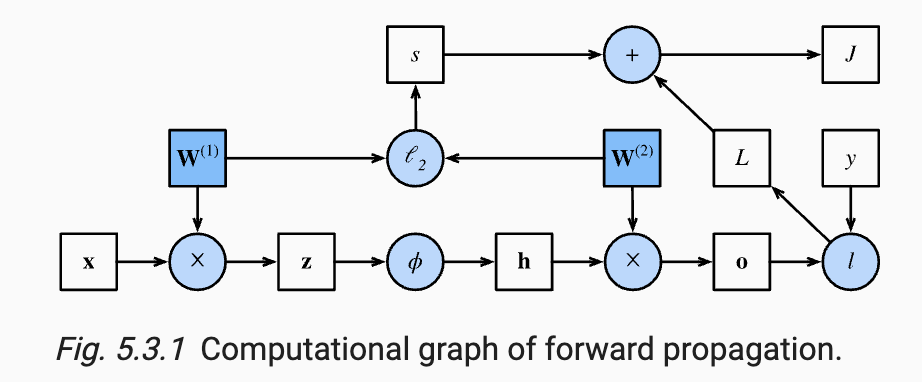
\includegraphics[keepaspectratio]{main_files/image.png}
\caption{image.png}
\end{figure}

    \paragraph{5.1.1.1. Limitations of Linear \mbox{}
Models}\label{limitations-of-linear-models}

    Linearity implies monotonicity, meaning that an increase in a feature
must either always increase or decrease the model's output. This
assumption often does not hold in real-world cases. For example, the
relationship between income and loan repayment likelihood is not linear.
Similarly, health prediction based on body temperature does not follow a
monotonic relationship.

Linear models fail in tasks like differentiating between cats and dogs,
where pixel intensity changes do not correlate directly to specific
categories. Nonlinearity is essential, and this is why deep neural
networks use hidden layers to learn both a representation of the data
and a linear predictor based on that representation.

    \paragraph{5.1.1.2. Incorporating Hidden \mbox{}
Layers}\label{incorporating-hidden-layers}

    We can overcome the limitations of linear models by incorporating one or
more hidden layers. The easiest way to do this is to stack many fully
connected layers on top of one another. Each layer feeds into the layer
above it until we generate outputs. This architecture is commonly called
a multilayer perceptron (MLP).

\begin{figure}
\centering
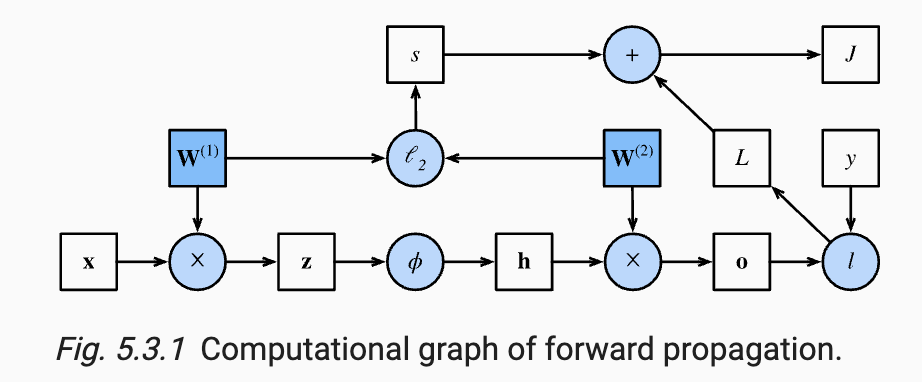
\includegraphics[keepaspectratio]{main_files/image.png}
\caption{image.png}
\end{figure}

    \paragraph{5.1.1.3. From Linear to \mbox{}
Nonlinear}\label{from-linear-to-nonlinear}

    As before, we denote by the matrix
\(\mathbf{X} \in \mathbb{R}^{n \times d}\) a minibatch of n examples
where each example has d inputs (features). For a one-hidden-layer MLP
whose hidden layer has h hidden units, we denote by
\(\mathbf{H} \in \mathbb{R}^{n \times h}\) the outputs of the hidden
layer, which are hidden representations. Since the hidden and output
layers are both fully connected, we have hidden-layer weights
\(\mathbf{W}^{(1)} \in \mathbb{R}^{d \times h}\) and biases
\(\mathbf{b}^{(1)} \in \mathbb{R}^{1 \times h}\), and output-layer
weights \(\mathbf{W}^{(2)} \in \mathbb{R}^{h \times q}\) and biases
\(\mathbf{b}^{(2)} \in \mathbb{R}^{1 \times q}\). This allows us to
calculate the outputs \(\mathbf{O} \in \mathbb{R}^{n \times q}\) of the
one-hidden-layer MLP as follows:

\(\mathbf{H} = \mathbf{X}\mathbf{W}^{(1)} + \mathbf{b}^{(1)}\),

\(\mathbf{O} = \mathbf{H}\mathbf{W}^{(2)} + \mathbf{b}^{(2)}\).

Note that after adding the hidden layer, our model now requires us to
track and update additional sets of parameters. So what have we gained
in exchange? You might be surprised to find out that---in the model
defined above---we gain nothing for our troubles! The reason is plain.
The hidden units above are given by an affine function of the inputs,
and the outputs (pre-softmax) are just an affine function of the hidden
units. An affine function of an affine function is itself an affine
function. Moreover, our linear model was already capable of representing
any affine function.

To see this formally we can just collapse out the hidden layer in the
above definition, yielding an equivalent single-layer model with
parameters
\(\mathbf{W} = \mathbf{W}^{(1)}\mathbf{W}^{(2)} and \mathbf{b} = \mathbf{b}^{(1)}\mathbf{W}^{(2)} + \mathbf{b}^{(2)}\):

\(\mathbf{O} = (\mathbf{X}\mathbf{W}^{(1)} + \mathbf{b}^{(1)})\mathbf{W}^{(2)} + \mathbf{b}^{(2)} = \mathbf{X}\mathbf{W}^{(1)}\mathbf{W}^{(2)} + \mathbf{b}^{(1)}\mathbf{W}^{(2)} + \mathbf{b}^{(2)} = \mathbf{X}\mathbf{W} + \mathbf{b}\).

In order to realize the potential of multilayer architectures, we need
one more key ingredient: a nonlinear activation function \sigma to be
applied to each hidden unit following the affine transformation. For
instance, a popular choice is the ReLU (rectified linear unit)
activation function (Nair and Hinton, 2010) \(\sigma(x) = \max(0, x)\)
operating on its arguments elementwise. The outputs of activation
functions \(\sigma(\cdot)\) are called activations. In general, with
activation functions in place, it is no longer possible to collapse our
MLP into a linear model:

\(\mathbf{H} = \sigma(\mathbf{X}\mathbf{W}^{(1)} + \mathbf{b}^{(1)})\),

\(\mathbf{O} = \mathbf{H}\mathbf{W}^{(2)} + \mathbf{b}^{(2)}\).

Since each row in \(\mathbf{X}\) corresponds to an example in the
minibatch, with some abuse of notation, we define the nonlinearity
\sigma to apply to its inputs in a rowwise fashion, i.e., one example at
a time. Note that we used the same notation for softmax when we denoted
a rowwise operation in Section 4.1.1.3. Quite frequently the activation
functions we use apply not merely rowwise but elementwise. That means
that after computing the linear portion of the layer, we can calculate
each activation without looking at the values taken by the other hidden
units.

To build more general MLPs, we can continue stacking such hidden layers,
e.g.,
\(\mathbf{H}^{(1)} = \sigma_1(\mathbf{X}\mathbf{W}^{(1)} + \mathbf{b}^{(1)})\)
and
\(\mathbf{H}^{(2)} = \sigma_2(\mathbf{H}^{(1)}\mathbf{W}^{(2)} + \mathbf{b}^{(2)})\),
one atop another, yielding ever more expressive models.

    \subsubsection*{5.1.2. Activation Functions}\label{activation-functions}

    Activation functions decide whether a neuron should be activated or not
by calculating the weighted sum and further adding bias to it. They are
differentiable operators for transforming input signals to outputs,
while most of them add nonlinearity. Because activation functions are
fundamental to deep learning, let's briefly survey some common ones.

    \paragraph{5.1.2.1. ReLU Function}\label{relu-function} \mbox{}

    \begin{tcolorbox}[breakable, size=fbox, boxrule=1pt, pad at break*=1mm,colback=cellbackground, colframe=cellborder]
\prompt{In}{incolor}{142}{\boxspacing}
\begin{Verbatim}[commandchars=\\\{\}]
\PY{n}{x} \PY{o}{=} \PY{n}{torch}\PY{o}{.}\PY{n}{arange}\PY{p}{(}\PY{o}{\PYZhy{}}\PY{l+m+mf}{8.0}\PY{p}{,} \PY{l+m+mf}{8.0}\PY{p}{,} \PY{l+m+mf}{0.1}\PY{p}{,} \PY{n}{requires\PYZus{}grad}\PY{o}{=}\PY{k+kc}{True}\PY{p}{)}
\PY{n}{y} \PY{o}{=} \PY{n}{torch}\PY{o}{.}\PY{n}{relu}\PY{p}{(}\PY{n}{x}\PY{p}{)}
\PY{n}{d2l}\PY{o}{.}\PY{n}{plot}\PY{p}{(}\PY{n}{x}\PY{o}{.}\PY{n}{detach}\PY{p}{(}\PY{p}{)}\PY{p}{,} \PY{n}{y}\PY{o}{.}\PY{n}{detach}\PY{p}{(}\PY{p}{)}\PY{p}{,} \PY{l+s+s1}{\PYZsq{}}\PY{l+s+s1}{x}\PY{l+s+s1}{\PYZsq{}}\PY{p}{,} \PY{l+s+s1}{\PYZsq{}}\PY{l+s+s1}{relu(x)}\PY{l+s+s1}{\PYZsq{}}\PY{p}{,} \PY{n}{figsize}\PY{o}{=}\PY{p}{(}\PY{l+m+mi}{5}\PY{p}{,} \PY{l+m+mf}{2.5}\PY{p}{)}\PY{p}{)}
\end{Verbatim}
\end{tcolorbox}

    \begin{center}
    \adjustimage{max size={0.9\linewidth}{0.9\paperheight}}{main_files/main_256_0.pdf}
    \end{center}
    { \hspace*{\fill} \\}
    
    \begin{tcolorbox}[breakable, size=fbox, boxrule=1pt, pad at break*=1mm,colback=cellbackground, colframe=cellborder]
\prompt{In}{incolor}{143}{\boxspacing}
\begin{Verbatim}[commandchars=\\\{\}]
\PY{n}{y}\PY{o}{.}\PY{n}{backward}\PY{p}{(}\PY{n}{torch}\PY{o}{.}\PY{n}{ones\PYZus{}like}\PY{p}{(}\PY{n}{x}\PY{p}{)}\PY{p}{,} \PY{n}{retain\PYZus{}graph}\PY{o}{=}\PY{k+kc}{True}\PY{p}{)}
\PY{n}{d2l}\PY{o}{.}\PY{n}{plot}\PY{p}{(}\PY{n}{x}\PY{o}{.}\PY{n}{detach}\PY{p}{(}\PY{p}{)}\PY{p}{,} \PY{n}{x}\PY{o}{.}\PY{n}{grad}\PY{p}{,} \PY{l+s+s1}{\PYZsq{}}\PY{l+s+s1}{x}\PY{l+s+s1}{\PYZsq{}}\PY{p}{,} \PY{l+s+s1}{\PYZsq{}}\PY{l+s+s1}{grad of relu}\PY{l+s+s1}{\PYZsq{}}\PY{p}{,} \PY{n}{figsize}\PY{o}{=}\PY{p}{(}\PY{l+m+mi}{5}\PY{p}{,} \PY{l+m+mf}{2.5}\PY{p}{)}\PY{p}{)}
\end{Verbatim}
\end{tcolorbox}

    \begin{center}
    \adjustimage{max size={0.9\linewidth}{0.9\paperheight}}{main_files/main_257_0.pdf}
    \end{center}
    { \hspace*{\fill} \\}
    
    \paragraph{5.1.2.2. Sigmoid Function}\label{sigmoid-function} \mbox{}

    \begin{tcolorbox}[breakable, size=fbox, boxrule=1pt, pad at break*=1mm,colback=cellbackground, colframe=cellborder]
\prompt{In}{incolor}{144}{\boxspacing}
\begin{Verbatim}[commandchars=\\\{\}]
\PY{n}{y} \PY{o}{=} \PY{n}{torch}\PY{o}{.}\PY{n}{sigmoid}\PY{p}{(}\PY{n}{x}\PY{p}{)}
\PY{n}{d2l}\PY{o}{.}\PY{n}{plot}\PY{p}{(}\PY{n}{x}\PY{o}{.}\PY{n}{detach}\PY{p}{(}\PY{p}{)}\PY{p}{,} \PY{n}{y}\PY{o}{.}\PY{n}{detach}\PY{p}{(}\PY{p}{)}\PY{p}{,} \PY{l+s+s1}{\PYZsq{}}\PY{l+s+s1}{x}\PY{l+s+s1}{\PYZsq{}}\PY{p}{,} \PY{l+s+s1}{\PYZsq{}}\PY{l+s+s1}{sigmoid(x)}\PY{l+s+s1}{\PYZsq{}}\PY{p}{,} \PY{n}{figsize}\PY{o}{=}\PY{p}{(}\PY{l+m+mi}{5}\PY{p}{,} \PY{l+m+mf}{2.5}\PY{p}{)}\PY{p}{)}
\end{Verbatim}
\end{tcolorbox}

    \begin{center}
    \adjustimage{max size={0.9\linewidth}{0.9\paperheight}}{main_files/main_259_0.pdf}
    \end{center}
    { \hspace*{\fill} \\}
    
    \begin{tcolorbox}[breakable, size=fbox, boxrule=1pt, pad at break*=1mm,colback=cellbackground, colframe=cellborder]
\prompt{In}{incolor}{146}{\boxspacing}
\begin{Verbatim}[commandchars=\\\{\}]
\PY{n}{x}\PY{o}{.}\PY{n}{grad}\PY{o}{.}\PY{n}{data}\PY{o}{.}\PY{n}{zero\PYZus{}}\PY{p}{(}\PY{p}{)}
\PY{n}{y}\PY{o}{.}\PY{n}{backward}\PY{p}{(}\PY{n}{torch}\PY{o}{.}\PY{n}{ones\PYZus{}like}\PY{p}{(}\PY{n}{x}\PY{p}{)}\PY{p}{,}\PY{n}{retain\PYZus{}graph}\PY{o}{=}\PY{k+kc}{True}\PY{p}{)}
\PY{n}{d2l}\PY{o}{.}\PY{n}{plot}\PY{p}{(}\PY{n}{x}\PY{o}{.}\PY{n}{detach}\PY{p}{(}\PY{p}{)}\PY{p}{,} \PY{n}{x}\PY{o}{.}\PY{n}{grad}\PY{p}{,} \PY{l+s+s1}{\PYZsq{}}\PY{l+s+s1}{x}\PY{l+s+s1}{\PYZsq{}}\PY{p}{,} \PY{l+s+s1}{\PYZsq{}}\PY{l+s+s1}{grad of sigmoid}\PY{l+s+s1}{\PYZsq{}}\PY{p}{,} \PY{n}{figsize}\PY{o}{=}\PY{p}{(}\PY{l+m+mi}{5}\PY{p}{,} \PY{l+m+mf}{2.5}\PY{p}{)}\PY{p}{)}
\end{Verbatim}
\end{tcolorbox}

    \begin{center}
    \adjustimage{max size={0.9\linewidth}{0.9\paperheight}}{main_files/main_260_0.pdf}
    \end{center}
    { \hspace*{\fill} \\}
    
    \paragraph{5.1.2.3. Tanh Function}\label{tanh-function} \mbox{}

    \begin{tcolorbox}[breakable, size=fbox, boxrule=1pt, pad at break*=1mm,colback=cellbackground, colframe=cellborder]
\prompt{In}{incolor}{147}{\boxspacing}
\begin{Verbatim}[commandchars=\\\{\}]
\PY{n}{y} \PY{o}{=} \PY{n}{torch}\PY{o}{.}\PY{n}{tanh}\PY{p}{(}\PY{n}{x}\PY{p}{)}
\PY{n}{d2l}\PY{o}{.}\PY{n}{plot}\PY{p}{(}\PY{n}{x}\PY{o}{.}\PY{n}{detach}\PY{p}{(}\PY{p}{)}\PY{p}{,} \PY{n}{y}\PY{o}{.}\PY{n}{detach}\PY{p}{(}\PY{p}{)}\PY{p}{,} \PY{l+s+s1}{\PYZsq{}}\PY{l+s+s1}{x}\PY{l+s+s1}{\PYZsq{}}\PY{p}{,} \PY{l+s+s1}{\PYZsq{}}\PY{l+s+s1}{tanh(x)}\PY{l+s+s1}{\PYZsq{}}\PY{p}{,} \PY{n}{figsize}\PY{o}{=}\PY{p}{(}\PY{l+m+mi}{5}\PY{p}{,} \PY{l+m+mf}{2.5}\PY{p}{)}\PY{p}{)}
\end{Verbatim}
\end{tcolorbox}

    \begin{center}
    \adjustimage{max size={0.9\linewidth}{0.9\paperheight}}{main_files/main_262_0.pdf}
    \end{center}
    { \hspace*{\fill} \\}
    
    \begin{tcolorbox}[breakable, size=fbox, boxrule=1pt, pad at break*=1mm,colback=cellbackground, colframe=cellborder]
\prompt{In}{incolor}{148}{\boxspacing}
\begin{Verbatim}[commandchars=\\\{\}]
\PY{n}{x}\PY{o}{.}\PY{n}{grad}\PY{o}{.}\PY{n}{data}\PY{o}{.}\PY{n}{zero\PYZus{}}\PY{p}{(}\PY{p}{)}
\PY{n}{y}\PY{o}{.}\PY{n}{backward}\PY{p}{(}\PY{n}{torch}\PY{o}{.}\PY{n}{ones\PYZus{}like}\PY{p}{(}\PY{n}{x}\PY{p}{)}\PY{p}{,}\PY{n}{retain\PYZus{}graph}\PY{o}{=}\PY{k+kc}{True}\PY{p}{)}
\PY{n}{d2l}\PY{o}{.}\PY{n}{plot}\PY{p}{(}\PY{n}{x}\PY{o}{.}\PY{n}{detach}\PY{p}{(}\PY{p}{)}\PY{p}{,} \PY{n}{x}\PY{o}{.}\PY{n}{grad}\PY{p}{,} \PY{l+s+s1}{\PYZsq{}}\PY{l+s+s1}{x}\PY{l+s+s1}{\PYZsq{}}\PY{p}{,} \PY{l+s+s1}{\PYZsq{}}\PY{l+s+s1}{grad of tanh}\PY{l+s+s1}{\PYZsq{}}\PY{p}{,} \PY{n}{figsize}\PY{o}{=}\PY{p}{(}\PY{l+m+mi}{5}\PY{p}{,} \PY{l+m+mf}{2.5}\PY{p}{)}\PY{p}{)}
\end{Verbatim}
\end{tcolorbox}

    \begin{center}
    \adjustimage{max size={0.9\linewidth}{0.9\paperheight}}{main_files/main_263_0.pdf}
    \end{center}
    { \hspace*{\fill} \\}
    
    \subsubsection*{5.1.3. Summary and
Discussion}\label{summary-and-discussion}

    We now know how to incorporate nonlinearities to build expressive
multilayer neural network architectures. In some ways, you have an
advantage over anyone working back then, because you can leverage
powerful open-source deep learning frameworks to build models rapidly,
using only a few lines of code. A secondary benefit is that ReLU is
significantly more amenable to optimization than the sigmoid or the tanh
function. Research in activation functions has not stopped. For
instance, the GELU activation function by Hendrycks and Gimpel (2016)
and the Swish activation function proposed in Ramachandran et al.~(2017)
can yield better accuracy in many cases.

    \subsection*{5.2. Implementation of Multilayer
Perceptrons}\label{implementation-of-multilayer-perceptrons}

    \begin{tcolorbox}[breakable, size=fbox, boxrule=1pt, pad at break*=1mm,colback=cellbackground, colframe=cellborder]
\prompt{In}{incolor}{149}{\boxspacing}
\begin{Verbatim}[commandchars=\\\{\}]
\PY{k+kn}{import} \PY{n+nn}{torch}
\PY{k+kn}{from} \PY{n+nn}{torch} \PY{k+kn}{import} \PY{n}{nn}
\PY{k+kn}{from} \PY{n+nn}{d2l} \PY{k+kn}{import} \PY{n}{torch} \PY{k}{as} \PY{n}{d2l}
\end{Verbatim}
\end{tcolorbox}

    \subsubsection*{5.2.1. Implementation from
Scratch}\label{implementation-from-scratch}

    \paragraph{5.2.1.1. Initializing Model \mbox{}
Parameters}\label{initializing-model-parameters}

    \begin{tcolorbox}[breakable, size=fbox, boxrule=1pt, pad at break*=1mm,colback=cellbackground, colframe=cellborder]
\prompt{In}{incolor}{150}{\boxspacing}
\begin{Verbatim}[commandchars=\\\{\}]
\PY{k}{class} \PY{n+nc}{MLPScratch}\PY{p}{(}\PY{n}{d2l}\PY{o}{.}\PY{n}{Classifier}\PY{p}{)}\PY{p}{:}
    \PY{k}{def} \PY{n+nf+fm}{\PYZus{}\PYZus{}init\PYZus{}\PYZus{}}\PY{p}{(}\PY{n+nb+bp}{self}\PY{p}{,} \PY{n}{num\PYZus{}inputs}\PY{p}{,} \PY{n}{num\PYZus{}outputs}\PY{p}{,} \PY{n}{num\PYZus{}hiddens}\PY{p}{,} \PY{n}{lr}\PY{p}{,} \PY{n}{sigma}\PY{o}{=}\PY{l+m+mf}{0.01}\PY{p}{)}\PY{p}{:}
        \PY{n+nb}{super}\PY{p}{(}\PY{p}{)}\PY{o}{.}\PY{n+nf+fm}{\PYZus{}\PYZus{}init\PYZus{}\PYZus{}}\PY{p}{(}\PY{p}{)}
        \PY{n+nb+bp}{self}\PY{o}{.}\PY{n}{save\PYZus{}hyperparameters}\PY{p}{(}\PY{p}{)}
        \PY{n+nb+bp}{self}\PY{o}{.}\PY{n}{W1} \PY{o}{=} \PY{n}{nn}\PY{o}{.}\PY{n}{Parameter}\PY{p}{(}\PY{n}{torch}\PY{o}{.}\PY{n}{randn}\PY{p}{(}\PY{n}{num\PYZus{}inputs}\PY{p}{,} \PY{n}{num\PYZus{}hiddens}\PY{p}{)} \PY{o}{*} \PY{n}{sigma}\PY{p}{)}
        \PY{n+nb+bp}{self}\PY{o}{.}\PY{n}{b1} \PY{o}{=} \PY{n}{nn}\PY{o}{.}\PY{n}{Parameter}\PY{p}{(}\PY{n}{torch}\PY{o}{.}\PY{n}{zeros}\PY{p}{(}\PY{n}{num\PYZus{}hiddens}\PY{p}{)}\PY{p}{)}
        \PY{n+nb+bp}{self}\PY{o}{.}\PY{n}{W2} \PY{o}{=} \PY{n}{nn}\PY{o}{.}\PY{n}{Parameter}\PY{p}{(}\PY{n}{torch}\PY{o}{.}\PY{n}{randn}\PY{p}{(}\PY{n}{num\PYZus{}hiddens}\PY{p}{,} \PY{n}{num\PYZus{}outputs}\PY{p}{)} \PY{o}{*} \PY{n}{sigma}\PY{p}{)}
        \PY{n+nb+bp}{self}\PY{o}{.}\PY{n}{b2} \PY{o}{=} \PY{n}{nn}\PY{o}{.}\PY{n}{Parameter}\PY{p}{(}\PY{n}{torch}\PY{o}{.}\PY{n}{zeros}\PY{p}{(}\PY{n}{num\PYZus{}outputs}\PY{p}{)}\PY{p}{)}
\end{Verbatim}
\end{tcolorbox}

    \paragraph{5.2.1.2. Model}\label{model} \mbox{}

    \begin{tcolorbox}[breakable, size=fbox, boxrule=1pt, pad at break*=1mm,colback=cellbackground, colframe=cellborder]
\prompt{In}{incolor}{151}{\boxspacing}
\begin{Verbatim}[commandchars=\\\{\}]
\PY{k}{def} \PY{n+nf}{relu}\PY{p}{(}\PY{n}{X}\PY{p}{)}\PY{p}{:}
    \PY{n}{a} \PY{o}{=} \PY{n}{torch}\PY{o}{.}\PY{n}{zeros\PYZus{}like}\PY{p}{(}\PY{n}{X}\PY{p}{)}
    \PY{k}{return} \PY{n}{torch}\PY{o}{.}\PY{n}{max}\PY{p}{(}\PY{n}{X}\PY{p}{,} \PY{n}{a}\PY{p}{)}
\end{Verbatim}
\end{tcolorbox}

    \begin{tcolorbox}[breakable, size=fbox, boxrule=1pt, pad at break*=1mm,colback=cellbackground, colframe=cellborder]
\prompt{In}{incolor}{152}{\boxspacing}
\begin{Verbatim}[commandchars=\\\{\}]
\PY{n+nd}{@d2l}\PY{o}{.}\PY{n}{add\PYZus{}to\PYZus{}class}\PY{p}{(}\PY{n}{MLPScratch}\PY{p}{)}
\PY{k}{def} \PY{n+nf}{forward}\PY{p}{(}\PY{n+nb+bp}{self}\PY{p}{,} \PY{n}{X}\PY{p}{)}\PY{p}{:}
    \PY{n}{X} \PY{o}{=} \PY{n}{X}\PY{o}{.}\PY{n}{reshape}\PY{p}{(}\PY{p}{(}\PY{o}{\PYZhy{}}\PY{l+m+mi}{1}\PY{p}{,} \PY{n+nb+bp}{self}\PY{o}{.}\PY{n}{num\PYZus{}inputs}\PY{p}{)}\PY{p}{)}
    \PY{n}{H} \PY{o}{=} \PY{n}{relu}\PY{p}{(}\PY{n}{torch}\PY{o}{.}\PY{n}{matmul}\PY{p}{(}\PY{n}{X}\PY{p}{,} \PY{n+nb+bp}{self}\PY{o}{.}\PY{n}{W1}\PY{p}{)} \PY{o}{+} \PY{n+nb+bp}{self}\PY{o}{.}\PY{n}{b1}\PY{p}{)}
    \PY{k}{return} \PY{n}{torch}\PY{o}{.}\PY{n}{matmul}\PY{p}{(}\PY{n}{H}\PY{p}{,} \PY{n+nb+bp}{self}\PY{o}{.}\PY{n}{W2}\PY{p}{)} \PY{o}{+} \PY{n+nb+bp}{self}\PY{o}{.}\PY{n}{b2}
\end{Verbatim}
\end{tcolorbox}

    \paragraph{5.2.1.3. Training}\label{training} \mbox{}

    \begin{tcolorbox}[breakable, size=fbox, boxrule=1pt, pad at break*=1mm,colback=cellbackground, colframe=cellborder]
\prompt{In}{incolor}{153}{\boxspacing}
\begin{Verbatim}[commandchars=\\\{\}]
\PY{n}{model} \PY{o}{=} \PY{n}{MLPScratch}\PY{p}{(}\PY{n}{num\PYZus{}inputs}\PY{o}{=}\PY{l+m+mi}{784}\PY{p}{,} \PY{n}{num\PYZus{}outputs}\PY{o}{=}\PY{l+m+mi}{10}\PY{p}{,} \PY{n}{num\PYZus{}hiddens}\PY{o}{=}\PY{l+m+mi}{256}\PY{p}{,} \PY{n}{lr}\PY{o}{=}\PY{l+m+mf}{0.1}\PY{p}{)}
\PY{n}{data} \PY{o}{=} \PY{n}{d2l}\PY{o}{.}\PY{n}{FashionMNIST}\PY{p}{(}\PY{n}{batch\PYZus{}size}\PY{o}{=}\PY{l+m+mi}{256}\PY{p}{)}
\PY{n}{trainer} \PY{o}{=} \PY{n}{d2l}\PY{o}{.}\PY{n}{Trainer}\PY{p}{(}\PY{n}{max\PYZus{}epochs}\PY{o}{=}\PY{l+m+mi}{10}\PY{p}{)}
\PY{n}{trainer}\PY{o}{.}\PY{n}{fit}\PY{p}{(}\PY{n}{model}\PY{p}{,} \PY{n}{data}\PY{p}{)}
\end{Verbatim}
\end{tcolorbox}

    \begin{center}
    \adjustimage{max size={0.9\linewidth}{0.9\paperheight}}{main_files/main_275_0.pdf}
    \end{center}
    { \hspace*{\fill} \\}
    
    \subsubsection*{5.2.2. Concise
Implementation}\label{concise-implementation}

    \paragraph{5.2.2.1. Model}\label{model} \mbox{}

    \begin{tcolorbox}[breakable, size=fbox, boxrule=1pt, pad at break*=1mm,colback=cellbackground, colframe=cellborder]
\prompt{In}{incolor}{154}{\boxspacing}
\begin{Verbatim}[commandchars=\\\{\}]
\PY{k}{class} \PY{n+nc}{MLP}\PY{p}{(}\PY{n}{d2l}\PY{o}{.}\PY{n}{Classifier}\PY{p}{)}\PY{p}{:}
    \PY{k}{def} \PY{n+nf+fm}{\PYZus{}\PYZus{}init\PYZus{}\PYZus{}}\PY{p}{(}\PY{n+nb+bp}{self}\PY{p}{,} \PY{n}{num\PYZus{}outputs}\PY{p}{,} \PY{n}{num\PYZus{}hiddens}\PY{p}{,} \PY{n}{lr}\PY{p}{)}\PY{p}{:}
        \PY{n+nb}{super}\PY{p}{(}\PY{p}{)}\PY{o}{.}\PY{n+nf+fm}{\PYZus{}\PYZus{}init\PYZus{}\PYZus{}}\PY{p}{(}\PY{p}{)}
        \PY{n+nb+bp}{self}\PY{o}{.}\PY{n}{save\PYZus{}hyperparameters}\PY{p}{(}\PY{p}{)}
        \PY{n+nb+bp}{self}\PY{o}{.}\PY{n}{net} \PY{o}{=} \PY{n}{nn}\PY{o}{.}\PY{n}{Sequential}\PY{p}{(}\PY{n}{nn}\PY{o}{.}\PY{n}{Flatten}\PY{p}{(}\PY{p}{)}\PY{p}{,} \PY{n}{nn}\PY{o}{.}\PY{n}{LazyLinear}\PY{p}{(}\PY{n}{num\PYZus{}hiddens}\PY{p}{)}\PY{p}{,}
                                 \PY{n}{nn}\PY{o}{.}\PY{n}{ReLU}\PY{p}{(}\PY{p}{)}\PY{p}{,} \PY{n}{nn}\PY{o}{.}\PY{n}{LazyLinear}\PY{p}{(}\PY{n}{num\PYZus{}outputs}\PY{p}{)}\PY{p}{)}
\end{Verbatim}
\end{tcolorbox}

    \paragraph{5.2.2.2. Training}\label{training} \mbox{}

    \begin{tcolorbox}[breakable, size=fbox, boxrule=1pt, pad at break*=1mm,colback=cellbackground, colframe=cellborder]
\prompt{In}{incolor}{155}{\boxspacing}
\begin{Verbatim}[commandchars=\\\{\}]
\PY{n}{model} \PY{o}{=} \PY{n}{MLP}\PY{p}{(}\PY{n}{num\PYZus{}outputs}\PY{o}{=}\PY{l+m+mi}{10}\PY{p}{,} \PY{n}{num\PYZus{}hiddens}\PY{o}{=}\PY{l+m+mi}{256}\PY{p}{,} \PY{n}{lr}\PY{o}{=}\PY{l+m+mf}{0.1}\PY{p}{)}
\PY{n}{trainer}\PY{o}{.}\PY{n}{fit}\PY{p}{(}\PY{n}{model}\PY{p}{,} \PY{n}{data}\PY{p}{)}
\end{Verbatim}
\end{tcolorbox}

    \begin{center}
    \adjustimage{max size={0.9\linewidth}{0.9\paperheight}}{main_files/main_280_0.pdf}
    \end{center}
    { \hspace*{\fill} \\}
    
    \subsubsection*{5.2.3. Summary}\label{summary}

    Now that we have more practice in designing deep networks, the step from
a single to multiple layers of deep networks does not pose such a
significant challenge any longer. Implementing MLPs from scratch is
nonetheless messy: naming and keeping track of the model parameters
makes it difficult to extend models. Moreover, if we implement the
network from scratch, it is much more difficult for the framework to
perform meaningful performance optimizations. Nonetheless, you have now
reached the state of the art of the late 1980s when fully connected deep
networks were the method of choice for neural network modeling.

    \subsubsection*{5.2.4. Exercises}\label{exercises}

    \begin{tcolorbox}[breakable, size=fbox, boxrule=1pt, pad at break*=1mm,colback=cellbackground, colframe=cellborder]
\prompt{In}{incolor}{157}{\boxspacing}
\begin{Verbatim}[commandchars=\\\{\}]
\PY{n}{hidden\PYZus{}units\PYZus{}list} \PY{o}{=} \PY{p}{[}\PY{l+m+mi}{64}\PY{p}{,} \PY{l+m+mi}{128}\PY{p}{,} \PY{l+m+mi}{256}\PY{p}{,} \PY{l+m+mi}{512}\PY{p}{]}
\PY{n}{accuracies} \PY{o}{=} \PY{p}{[}\PY{p}{]}

\PY{k}{for} \PY{n}{num\PYZus{}hiddens} \PY{o+ow}{in} \PY{n}{hidden\PYZus{}units\PYZus{}list}\PY{p}{:}
    \PY{n}{model} \PY{o}{=} \PY{n}{MLPScratch}\PY{p}{(}\PY{n}{num\PYZus{}inputs}\PY{o}{=}\PY{l+m+mi}{784}\PY{p}{,} \PY{n}{num\PYZus{}outputs}\PY{o}{=}\PY{l+m+mi}{10}\PY{p}{,} \PY{n}{num\PYZus{}hiddens}\PY{o}{=}\PY{n}{num\PYZus{}hiddens}\PY{p}{,} \PY{n}{lr}\PY{o}{=}\PY{l+m+mf}{0.1}\PY{p}{)}
    \PY{n}{trainer} \PY{o}{=} \PY{n}{d2l}\PY{o}{.}\PY{n}{Trainer}\PY{p}{(}\PY{n}{max\PYZus{}epochs}\PY{o}{=}\PY{l+m+mi}{10}\PY{p}{)}
    \PY{n}{data} \PY{o}{=} \PY{n}{d2l}\PY{o}{.}\PY{n}{FashionMNIST}\PY{p}{(}\PY{n}{batch\PYZus{}size}\PY{o}{=}\PY{l+m+mi}{256}\PY{p}{)}
    \PY{n}{accuracy} \PY{o}{=} \PY{n}{trainer}\PY{o}{.}\PY{n}{fit}\PY{p}{(}\PY{n}{model}\PY{p}{,} \PY{n}{data}\PY{p}{)}
    \PY{n}{accuracies}\PY{o}{.}\PY{n}{append}\PY{p}{(}\PY{n}{accuracy}\PY{p}{)}
\end{Verbatim}
\end{tcolorbox}

    \begin{center}
    \adjustimage{max size={0.9\linewidth}{0.9\paperheight}}{main_files/main_284_0.pdf}
    \end{center}
    { \hspace*{\fill} \\}
    
    \begin{center}
    \adjustimage{max size={0.9\linewidth}{0.9\paperheight}}{main_files/main_284_1.pdf}
    \end{center}
    { \hspace*{\fill} \\}
    
    \begin{center}
    \adjustimage{max size={0.9\linewidth}{0.9\paperheight}}{main_files/main_284_2.pdf}
    \end{center}
    { \hspace*{\fill} \\}
    
    \begin{center}
    \adjustimage{max size={0.9\linewidth}{0.9\paperheight}}{main_files/main_284_3.pdf}
    \end{center}
    { \hspace*{\fill} \\}
    
    \subsection*{5.3. Forward Propagation, Backward Propagation, and
Computational
Graphs}\label{forward-propagation-backward-propagation-and-computational-graphs}

    \subsubsection*{5.3.1. Forward Propagation}\label{forward-propagation}

    Forward propagation (or forward pass) refers to the calculation and
storage of intermediate variables (including outputs) for a neural
network in order from the input layer to the output layer. We now work
step-by-step through the mechanics of a neural network with one hidden
layer. This may seem tedious but in the eternal words of funk virtuoso
James Brown, you must ``pay the cost to be the boss''.

For the sake of simplicity, let's assume that the input example is
\(\mathbf{x} \in \mathbb{R}^{d}\) and that our hidden layer does not
include a bias term. Here the intermediate variable is:

\(\mathbf{z} = \mathbf{W}^{(1)}\mathbf{x}\),

where \(\mathbf{W}^{(1)} \in \mathbb{R}^{h \times d}\) is the weight
parameter of the hidden layer. After running the intermediate variable
\(\mathbf{z} \in \mathbb{R}^{h}\) through the activation function
\(\phi\), we obtain our hidden activation vector of length \(h\):

\(\mathbf{h} = \phi(\mathbf{z})\).

The hidden layer output \(\mathbf{h}\) is also an intermediate variable.
Assuming that the parameters of the output layer possess only a weight
of \(\mathbf{W}^{(2)} \in \mathbb{R}^{q \times h}\), we can obtain an
output layer variable with a vector of length \(q\):

\(\mathbf{o} = \mathbf{W}^{(2)}\mathbf{h}\).

Assuming that the loss function is \(l\) and the example label is \(y\),
we can then calculate the loss term for a single data example,

\(L = l(\mathbf{o}, y)\).

As we will see the definition of \(\ell_2\) regularization to be
introduced later, given the hyperparameter \(\lambda\), the
regularization term is

\(s = \frac{\lambda}{2} \left( \|\mathbf{W}^{(1)}\|_F^2 + \|\mathbf{W}^{(2)}\|_F^2 \right)\),

where the Frobenius norm of the matrix is simply the \(\ell_2\) norm
applied after flattening the matrix into a vector. Finally, the model's
regularized loss on a given data example is:

\(J = L + s\).

We refer to \(J\) as the objective function in the following discussion.

    \subsubsection*{5.3.2. Computational Graph of Forward
propagation}\label{computational-graph-of-forward-propagation}

    Plotting computational graphs helps us visualize the dependencies of
operators and variables within the calculation. Fig. 5.3.1 contains the
graph associated with the simple network described above, where squares
denote variables and circles denote operators. The lower-left corner
signifies the input and the upper-right corner is the output. Notice
that the directions of the arrows (which illustrate data flow) are
primarily rightward and upward.

\begin{figure}
\centering
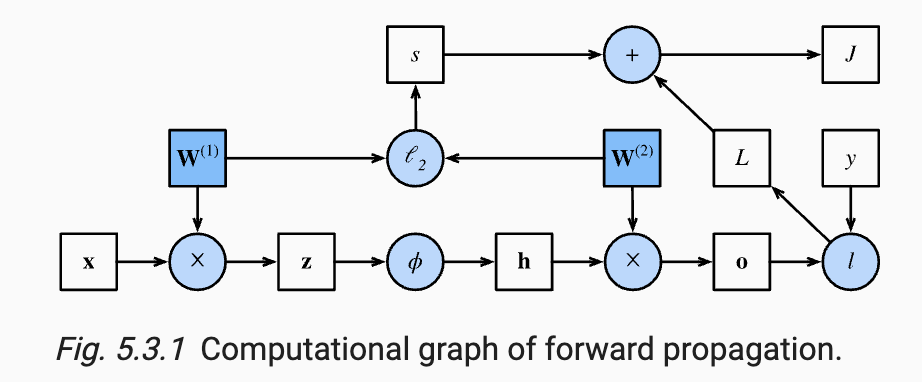
\includegraphics[keepaspectratio]{main_files/image.png}
\caption{image.png}
\end{figure}

    \subsubsection*{5.3.3. Backpropagation}\label{backpropagation}

    Backpropagation refers to the method of calculating the gradient of
neural network parameters. In short, the method traverses the network in
reverse order, from the output to the input layer, according to the
chain rule from calculus. The algorithm stores any intermediate
variables (partial derivatives) required while calculating the gradient
with respect to some parameters. Assume that we have functions
\(Y = f(X)\) and \(Z = g(Y)\), in which the input and the output
\(X, Y, Z\) are tensors of arbitrary shapes. By using the chain rule, we
can compute the derivative of \(Z\) with respect to \(X\) via

\(\frac{\partial Z}{\partial X} = \prod \left( \frac{\partial Z}{\partial Y}, \frac{\partial Y}{\partial X} \right)\).

Here we use the prod operator to multiply its arguments after the
necessary operations, such as transposition and swapping input
positions, have been carried out. For vectors, this is straightforward:
it is simply matrix-matrix multiplication. For higher-dimensional
tensors, we use the appropriate counterpart. The operator prod hides all
the notational overhead.

Recall that the parameters of the simple network with one hidden layer,
whose computational graph is in Fig. 5.3.1, are \(\mathbf{W}^{(1)}\) and
\(\mathbf{W}^{(2)}\). The objective of backpropagation is to calculate
the gradients \(\frac{\partial J}{\partial \mathbf{W}^{(1)}}\) and
\(\frac{\partial J}{\partial \mathbf{W}^{(2)}}\). To accomplish this, we
apply the chain rule and calculate, in turn, the gradient of each
intermediate variable and parameter. The order of calculations is
reversed relative to those performed in forward propagation, since we
need to start with the outcome of the computational graph and work our
way towards the parameters. The first step is to calculate the gradients
of the objective function \(J = L + s\) with respect to the loss term
\(L\) and the regularization term \(s\):

\(\frac{\partial J}{\partial L} = 1 \quad \text{and} \quad \frac{\partial J}{\partial s} = 1\).

Next, we compute the gradient of the objective function with respect to
variable of the output layer o according to the chain rule:

\(\frac{\partial J}{\partial \mathbf{o}} = \prod \left( \frac{\partial J}{\partial L}, \frac{\partial L}{\partial \mathbf{o}} \right) = \frac{\partial L}{\partial \mathbf{o}} \in \mathbb{R}^{q}\).

Next, we calculate the gradients of the regularization term with respect
to both parameters:

\(\frac{\partial s}{\partial \mathbf{W}^{(1)}} = \lambda \mathbf{W}^{(1)} \quad \text{and} \quad \frac{\partial s}{\partial \mathbf{W}^{(2)}} = \lambda \mathbf{W}^{(2)}\).

Now we are able to calculate the gradient
\(\frac{\partial J}{\partial \mathbf{W}^{(2)}} \in \mathbb{R}^{q \times h}\)
of the model parameters closest to the output layer. Using the chain
rule yields:

\(\frac{\partial J}{\partial \mathbf{W}^{(2)}} = \prod \left( \frac{\partial J}{\partial \mathbf{o}}, \frac{\partial \mathbf{o}}{\partial \mathbf{W}^{(2)}} \right) + \prod \left( \frac{\partial s}{\partial s}, \frac{\partial s}{\partial \mathbf{W}^{(2)}} \right) = \frac{\partial J}{\partial \mathbf{o}} \mathbf{h}^{\top} + \lambda \mathbf{W}^{(2)}\).

To obtain the gradient with respect to \(\mathbf{W}^{(1)}\) we need to
continue backpropagation along the output layer to the hidden layer. The
gradient with respect to the hidden layer output
\(\frac{\partial J}{\partial \mathbf{h}} \in \mathbb{R}^{h}\) is given
by

\(\frac{\partial J}{\partial \mathbf{h}} = \prod \left( \frac{\partial J}{\partial \mathbf{o}}, \frac{\partial \mathbf{o}}{\partial \mathbf{h}} \right) = \mathbf{W}^{(2)} \top \frac{\partial J}{\partial \mathbf{o}}\).

Since the activation function \(\phi\) applies elementwise, calculating
the gradient
\(\frac{\partial J}{\partial \mathbf{z}} \in \mathbb{R}^{h}\) of the
intermediate variable \(\mathbf{z}\) requires that we use the
elementwise multiplication operator, which we denote by \(\odot\):

\(\frac{\partial J}{\partial \mathbf{z}} = \prod \left( \frac{\partial J}{\partial \mathbf{h}}, \frac{\partial \mathbf{h}}{\partial \mathbf{z}} \right) = \frac{\partial J}{\partial \mathbf{h}} \odot \phi{\prime}(\mathbf{z})\).

Finally, we can obtain the gradient
\(\frac{\partial J}{\partial \mathbf{W}^{(1)}} \in \mathbb{R}^{h \times d}\)
of the model parameters closest to the input layer. According to the
chain rule, we get

\(\frac{\partial J}{\partial \mathbf{W}^{(1)}} = \prod \left( \frac{\partial J}{\partial \mathbf{z}}, \frac{\partial \mathbf{z}}{\partial \mathbf{W}^{(1)}} \right) + \prod \left( \frac{\partial s}{\partial s}, \frac{\partial s}{\partial \mathbf{W}^{(1)}} \right) = \frac{\partial J}{\partial \mathbf{z}} \mathbf{x}^{\top} + \lambda \mathbf{W}^{(1)}\).

    \subsubsection*{5.3.4. Training Neural
Networks}\label{training-neural-networks}

    When training neural networks, forward and backward propagation depend
on each other. In forward propagation, we traverse the computational
graph in the direction of dependencies, and the variables are then used
for backpropagation, where the compute order on the graph is reversed.
When training neural networks, once model parameters are initialized, we
alternate forward propagation with backpropagation, updating model
parameters using gradients given by backpropagation. Note that
backpropagation reuses the stored intermediate values from forward
propagation to avoid duplicate calculations. This is also one of the
reasons why training requires significantly more memory than plain
prediction. Training deeper networks using larger batch sizes more
easily leads to out-of-memory errors.

    \subsubsection*{5.3.5. Summary}\label{summary}

    Forward propagation sequentially calculates and stores intermediate
variables within the computational graph defined by the neural network.
Backpropagation sequentially calculates and stores the gradients of
intermediate variables and parameters within the neural network in the
reversed order. When training deep learning models, forward propagation
and backpropagation are interdependent, and training requires
significantly more memory than prediction.


    % Add a bibliography block to the postdoc
    
    
    
\end{document}
